%% 
%% Copyright 2007-2024 Elsevier Ltd
%% 
%% This file is part of the 'Elsarticle Bundle'.
%% ---------------------------------------------
%% 
%% It may be distributed under the conditions of the LaTeX Project Public
%% License, either version 1.3 of this license or (at your option) any
%% later version.  The latest version of this license is in
%%    http://www.latex-project.org/lppl.txt
%% and version 1.3 or later is part of all distributions of LaTeX
%% version 1999/12/01 or later.
%% 
%% The list of all files belonging to the 'Elsarticle Bundle' is
%% given in the file `manifest.txt'.
%% 
%% Template article for Elsevier's document class `elsarticle'
%% with numbered style bibliographic references
%% SP 2008/03/01
%% $Id: elsarticle-template-num.tex 249 2024-04-06 10:51:24Z rishi $
%%
\documentclass[preprint,12pt,sort&compress]{elsarticle}
% \documentclass[final,5p,times,twocolumn,sort&compress]{elsarticle}

%% Custom packages
\usepackage[super]{nth}
\usepackage{amsfonts,amsthm,cancel,siunitx,calculator,calc,mathtools,empheq,latexsym}
\usepackage[version=4]{mhchem}
\usepackage[hyphens]{url} % allow line breaks in urls
\usepackage[breaklinks=true]{hyperref} % allow breakable links
\usepackage{booktabs,multicol,multirow,tabularx,array}
\usepackage[official]{eurosym}
\usepackage{subcaption}
\usepackage{placeins}
\usepackage{float}
\usepackage{tabularx}
\usepackage{enumitem}
\usepackage{bm}
\usepackage{todonotes}

\newcolumntype{R}[1]{>{\raggedleft\arraybackslash}p{#1}}

\graphicspath{
    {figures/}
  }
\DeclareGraphicsExtensions{.pdf,.jpeg,.jpg,.png}

%% Use the option review to obtain double line spacing
%% \documentclass[authoryear,preprint,review,12pt]{elsarticle}

%% Use the options 1p,twocolumn; 3p; 3p,twocolumn; 5p; or 5p,twocolumn
%% for a journal layout:
%% \documentclass[final,1p,times]{elsarticle}
%% \documentclass[final,1p,times,twocolumn]{elsarticle}
%% \documentclass[final,3p,times]{elsarticle}
%% \documentclass[final,3p,times,twocolumn]{elsarticle}
%% \documentclass[final,5p,times]{elsarticle}
%% \documentclass[final,5p,times,twocolumn]{elsarticle}

%% For including figures, graphicx.sty has been loaded in
%% elsarticle.cls. If you prefer to use the old commands
%% please give \usepackage{epsfig}

%% The amssymb package provides various useful mathematical symbols
\usepackage{amssymb}
%% The amsmath package provides various useful equation environments.
\usepackage{amsmath}
%% The amsthm package provides extended theorem environments
%% \usepackage{amsthm}

%% The lineno packages adds line numbers. Start line numbering with
%% \begin{linenumbers}, end it with \end{linenumbers}. Or switch it on
%% for the whole article with \linenumbers.
\usepackage{lineno}
\linenumbers

\journal{Nuclear Physics B}

\begin{document}

\begin{frontmatter}

%% Title, authors and addresses

%% use the tnoteref command within \title for footnotes;
%% use the tnotetext command for theassociated footnote;
%% use the fnref command within \author or \affiliation for footnotes;
%% use the fntext command for theassociated footnote;
%% use the corref command within \author for corresponding author footnotes;
%% use the cortext command for theassociated footnote;
%% use the ead command for the email address,
%% and the form \ead[url] for the home page:
%% \title{Title\tnoteref{label1}}
%% \tnotetext[label1]{}
%% \author{Name\corref{cor1}\fnref{label2}}
%% \ead{email address}
%% \ead[url]{home page}
%% \fntext[label2]{}
%% \cortext[cor1]{}
%% \affiliation{organization={},
%%             addressline={},
%%             city={},
%%             postcode={},
%%             state={},
%%             country={}}
%% \fntext[label3]{}

\title{The role of Projects of Common Interest in reaching Europe's energy policy targets}

%% use optional labels to link authors explicitly to addresses:
%% \author[label1,label2]{}
%% \affiliation[label1]{organization={},
%%             addressline={},
%%             city={},
%%             postcode={},
%%             state={},
%%             country={}}
%%
%% \affiliation[label2]{organization={},
%%             addressline={},
%%             city={},
%%             postcode={},
%%             state={},
%%             country={}}

\author[affi1]{Bobby Xiong\corref{cor1}} %% Author name
\author[affil1]{Iegor Riepin}
\author[affil1]{Tom Brown}

\cortext[cor1]{Corresponding author: \href{mailto:xiong@tu-berlin.de}{xiong@tu-berlin.de}}

%% Author affiliation
\affiliation[affi1]{organization={TU Berlin, Department of Digital Transformation in Energy Systems},
            % addressline={},
            city={Berlin},
            % postcode={},
            % state={},
            country={Germany}}

%% Abstract
\begin{abstract}
  OLD OUTDATED IEW-EXTENDED-ABSTRACT. The European Union (EU) aims to achieve climate-neutrality by 2050, with ambitious 2030 target, such as \SI{55}{\percent} greenhouse gas emissions reduction compared to 1990 levels, \SI{10}{Mt} p.a. of a domestic green \ce{H2} production, and \SI{50}{Mt} p.a. of \ce{CO2} injection capacity, which should be sequestered within the EU. 
  The European Commission selects so-called Projects of Common Interest (PCI) and Projects of Mutual Interest (PMI)---a large infrastructure projects for electricity, hydrogen and \ce{CO2} transport, and storage---that are of transnational importance as they link the energy systems of European countries.
  In this work, we evaluate the impact of PCI-PMI projects for the European energy system and EU energy policies. To achieve this, we investigate how delays in these projects could affect the EU's policy targets and examine potential conflicts between various policy objectives and the overarching greenhouse gas reduction goal. 
  Our preliminary results for 2030 indicate that policy targets can be met even without PCI-PMI projects; however, these projects offer additional benefits: (i) \ce{H2} pipelines enhance the affordability and distribution of green \ce{H2}, thereby jumpstarting the hydrogen economy, and (ii) \ce{CO2} transport projects connect major industrial emissions to offshore sequestration sites in the North Sea.
  In our future work, we will analyse long-term pathway effects up to 2050, and incorporate hybrid interconnectors and \ce{CO2} shipping routes from the PCI-PMI list. 
  Overall, our findings highlight the critical interplay between cross-border cooperation, infrastructure investments, and policy targets in the European energy transition across all sectors.
\end{abstract}

% %%Graphical abstract
% \begin{graphicalabstract}
% %\includegraphics{grabs}
% \end{graphicalabstract}

% %%Research highlights
% \begin{highlights}
% \item Research highlight 1
% \item Research highlight 2
% \end{highlights}

%% Keywords
\begin{keyword}
energy system modelling \sep policy targets \sep infrastructure \sep resilience \sep hydrogen \sep carbon \sep Europe 
%% keywords here, in the form: keyword \sep keyword

%% PACS codes here, in the form: \PACS code \sep code

%% MSC codes here, in the form: \MSC code \sep code
%% or \MSC[2008] code \sep code (2000 is the default)

\end{keyword}

\end{frontmatter}

%% Add \usepackage{lineno} before \begin{document} and uncomment 
%% following line to enable line numbers
%% \linenumbers

%% main text
%%

%% Use \section commands to start a section.
\section*{List of abbreviations}

\begin{itemize}[left=0pt, label={}, itemsep=0pt, parsep=0pt, topsep=0pt]
  \item \textbf{AC} \enspace Alternating Current
  \item \textbf{API} \enspace Application Programming Interface
  \item \textbf{CC} \enspace Carbon Capture
  \item \textbf{CU} \enspace Carbon Utilisation
  \item \textbf{CS} \enspace Carbon Storage
  \item \textbf{CCUS} \enspace Carbon Capture, Utilisation, and Storage
  \item \textbf{DAC} \enspace Direct Air Capture
  \item \textbf{DC} \enspace Direct Current
  \item \textbf{EU} \enspace European Union
  \item \textbf{GHG} \enspace Greenhouse gas
  \item \textbf{NEP} \enspace Netzentwicklungsplan (German grid development plan)
  \item \textbf{NUTS} \enspace Nomenclature of Territorial Units for Statistics
  \item \textbf{PCI} \enspace Projects of Common Interest
  \item \textbf{PMI} \enspace Projects of Mutual Interest
  \item \textbf{REST} \enspace Representational State Transfer 
  \item \textbf{tsam} \enspace Time Series Aggregation Module
  \item \textbf{TYNDP} \enspace Ten-Year Network Development Plan
  \item \textbf{WACC} \enspace Weighted Average Cost of Capital

\end{itemize}

\section{Introduction}
\label{sec:introduction}
WORK-IN-PROGRESS-INCOMPLETE. On the pathway to a climate-neutral Europe by 2050, the European Union (EU) has set ambitious targets for 2030. These targets include a reduction of \SI{55}{\percent} in greenhouse gas emissions compared to 1990 levels \cite{europeancommissionFit55Delivering2021}, \SI{10}{Mt} p.a. domestic green \ce{H2} production \cite{europeancommissionREPowerEUPlanCommunication2022}, and \SI{50}{Mt} p.a. of \ce{CO2} injection capacity with sequestration in within the EU \cite{europeanparliamentRegulationEU20242024}.

To support reaching these targets, the European Commission bi-annually identifies a list of Projects of Common Interest (PCI), which are key cross-border infrastructure projects that link the energy systems of the EU members, including transmission and storage projects for electricity, hydrogen and \ce{CO2} \cite{europeancommissionCommissionDelegatedRegulation2023}. 
The pool of project sutable for PCI status is based on projects submitted by transmission system operators, consortia, or third parties. Projects of Mutual Interest (PMI) further include cooperations with countries outside the EU, such as Norway or the United Kingdom. With a PCI-PMI status, project awardees receive strong political support and are, amongst others, eligible for financial support (e.g. through funding of the Connecting Europe Facility) and see accelerated permitting processes. On the other hand, project promoters are obliged to undergo comprehensive reporting and monitoring processes. 
In order for projects to be eligible for PCI-PMI status, their \textit{potential benefits need to outweigh their costs} \cite{europeancommissionCommissionDelegatedRegulation2023}. Given the political and lighthouse character, these projects are highly likely to be implemented. However, any large infrastructure project, including PCI-PMI projects, commonly face delays due to permitting, financing, procurement bottlenecks, etc. \cite
{acerConsolidatedReportProgress2023}.

\begin{itemize}
  \item Net zero law by 2050 \citet{europeanparliamentRegulationEU20242024}
\end{itemize}

\subsection{Fuels, carriers, targets}
\paragraph{Hydrogen (\ce{H2})}
\begin{itemize}
  \item "net zero systems: H2 feedstock for synthetic fuels, fuel transportation sector, feedstock and heat source in industry," \cite{greevenbroekLittleLoseCase2024}, \cite{beresWillHydrogenSynthetic2024}
\end{itemize}

\subsection{Projects of Common/Mutual Interest}


\newpage
\section{Literature review}
\label{sec:literature_review}
We structure the literature review into three main sections: (i) the value of \ce{CO2} and \ce{H2} in low-carbon energy systems and (iii) addressing uncertainty in energy system models. Based on this review, identify research gaps and position our work as a novel contribution to the current state of the art (iii).

\subsection{The value of \ce{CO2} and \ce{H2} in low-carbon energy systems} 
A growing body of literature has been investigating the long-term role of \ce{H2} and \ce{CO2} in low-carbon or net-zero energy systems. Both carriers see their primary value outside the electricity sector, i.e., in the decarbonisation of hard-to-abate sectors such as industry, transport, shipping, and aviation \cite{reigstadMovingLowcarbonHydrogen2022}. While there are direct use cases for \ce{H2} in the industry sector such as steel production, it is primarily expected to serve as a precursor for synthetic fuels, including methanol, Fischer-Tropsch fuels (e.g. synthetic kerosene and naphta) and methane. The demand for these fuels is driven by the aviation, shipping, industry, and agriculture sectors \cite{neumannPotentialRoleHydrogen2023}. To produce these carbonaceous fuels, \ce{CO2} is required as a feedstock (Carbon Utilisation --- CU). This \ce{CO2} can be captured from the atmosphere via Direct Air Capture (DAC) or from industrial and process emissions (e.g. cement, steel, ammonia production) in combination with Carbon Capture (CC) units.

Béres et al. \cite{beresWillHydrogenSynthetic2024} evaluate the interaction between electricity, \ce{H2}, and synthetic fuel demand by linking the JRC-EU-TIMES long-term energy system model with PLEXOS. In their findings, \ce{H2} production varies between 42 (1400 TWh) and 66 Mt (2200 TWh) p.a. in 2050. 

Van Greevenbroek et al. \cite{greevenbroekLittleLoseCase2024} investigate the cost-optimal development of green \ce{H2} by assessing the near-optimal space of an extensive scenario set. They find a moderate level of green \ce{H2} production is cost-optimal, with production levels depending primarily on the availability of green fuel imports and carbon, capture, and storage. Eliminating green \ce{H2} entirely would come at a total system cost increase of \SI{2}{\percent}. 

By including \ce{H2} and \ce{CO2} transport infrastructure, additional benefits and net cost-savings can be unlocked in a sector-coupled system.

Neumann et al. \cite{neumannPotentialRoleHydrogen2023} examine the interaction between electricity grid expansion and a European-wide deployment of hydrogen pipelines in a net-zero system (new and retrofitting of existing gas pipelines). While \ce{H2} pipelines are not essential, their build-out can significantly reduce system costs by up to 26 bn. \euro{} p.a. (\SI{3.4}{\percent} of annual CAPEX and OPEX) by connecting regions with excessive renewable potential to storage sites and load centres. 
Extending their previous work, Neumann et al. \cite{neumannEnergyImportsInfrastructure2024} investigate the trade-off between relying on different energy import strategies and domestric infrastructure build-out. By coupling the global energy supply chain model TRACE \cite{hamppImportOptionsChemical2023} and the sector-coupled PyPSA-Eur model, they assess different energy vector import combinations (e.g. electricity, \ce{H2} or \ce{H2} derivatives) and their impact on Europe's infrastructural needs. Depending on the import costs, they observe up to \SI{14}{\percent} in system cost savings. Further, with an increasing share of \ce{H2} imports, the need for domestic \ce{H2} pipelines would decrease. 

In a study by Kontouris et al. \cite{kountourisUnifiedEuropeanHydrogen2024}, the authors explore pathways for a potential integrated hydrogen infrastructure in Europe while considering sector-coupling and energy imports. Using the European energy system model Balmorel \cite{wieseBalmorelOpenSource2018}, the authors implement three scenarios varying between domestic and imported \ce{H2} levels as well as \ce{H2} production technologies. In their findings they identify main \ce{H2} transport corridors from Spain and France, Ireland and the United Kingdom, Italy, and Southeastern Europe. When synergies through sector-coupling are exploited, domestic \ce{H2} production can be competitive, seeing an increase in up to \SI{3}{\percent} in system costs.

Fleiter et al. \cite{fleiterHydrogenInfrastructureFuture2025} use a mixed simulation and optimisation method to model \ce{H2} uptake and transport by coupling three models, (i) FORECAST for buildings and industry, (ii) ALADIN for transport together with (iii) the European energy system model Enertile. Total demand for \ce{H2} ranges from \SI{690}{TWh} to \SI{2800}{TWh} in 2050, \SI{600}{TWh} to \SI{1400}{TWh} for synthetic fuels. In their study, the  chemical and steel industry in Northwest Europe (incl. western regions of Germany, Netherlands and northern regions of Belgium), display a demand of more than \SI{100}{TWh} each. With regard to crossborder transport, they mainly obser hydrogen flows from Norway, UK and Ireland to continental Europe (around \SI{53}{TWh} to \SI{72}{TWh}). Depending on the scenario, the Iberian Peninsula exports around \SI{72}{TWh} to \SI{235}{TWh} via and to France.

On the carbon networks side, Bakken and Velken \cite{bakkenLinearModelsOptimization2008} formulate linear models for the optimisation of \ce{CO2} infrastructure, including pipelines, shipping, \ce{CO2} capture, and storage and demonstrate the applicability in a regional case study for Norway.
Hofmann et al. \cite{hofmannH2CO2Network2025} address previous research gap in assessing the interaction between \ce{H2} and \ce{CO2} infrastructure, by combining the the production, transport, storage, and utilisation of both \ce{H2}, \ce{CO2} and their products. They specifically raise the question whether \ce{H2} should be transported to \ce{CO2} point sources or vice versa. They find that most cost savings can be achieved in a hybrid setup where both networks are present, as the \ce{CO2} network complements the \ce{H2} network by promoting carbon capture from point sources and reducing reliance on Direct Air Capture (DAC).
 
\subsection{Addressing uncertainty in energy system models}
While the previous section have examined the value of \ce{CO2} and \ce{H2} in low-carbon energy systems, they do not take into account potential uncertainties regarding future policy targets or infrastructure build-outs. 
Energy system models can address such uncertainties through a range of approaches, including scenario analysis, sensitivity analysis, stochastic programming, and regret-based methods. Within the scope of this research, we focus on the (deterministic) scenario analysis and regret-based methods, as they are particularly suitable for complex, large-scale, sector-coupled system models.

\paragraph{Regret analysis}
A regret analysis is a common and widely established approach in economics that systematically evaluates the regret, i.e., additional system costs, incurred by not having made the optimal decision in hindsight. Usually, a regret-analysis is designed in two steps, first, a set of scenarios is defined, which represent different future developments, such as policy targets, infrastructure build-out, or technology costs. In a second step, the performance of first-stage investment is evaluated under the realisation of second-stage or short-term realisations of the future \cite{salvatoreManagerialEconomicPrinciples2008}. It is particularly useful in energy system modelling, where future uncertainties can significantly impact the performance of investments in infrastructure and technologies.

Möbius and Riepin \cite{mobiusRegretAnalysisInvestment2020} investigate the regret of investment decisions into electricity generation capacities, by developing a two-stage, stochastic cost-minimisation model of the European electricity and gas markets. In the first stage, the model determines optimal investment decisions, accounting for three TYNDP scenarios, while the second step solves the optimal dispatch for all assets in the electricity and gas sector. They find that ignoring uncertainty may result in investment decisions that lead to higher costs and regrets. 

Van der Weijde and Hobbes \cite{vanderweijdeEconomicsPlanningElectricity2012} demonstrate the importance of considering uncertainty in energy system models, by applying a two-stage optimisation model to evaluate grid reinforcements in Great Britain. Including the status quo scenario, they consider six scenarios, which represent different future developments of electricity demand, generation, fuel, and \ce{CO2} prices. As part of their study, they calculate the regret for given first-stage transmission decisions under the realisation of second-stage scenarios. Note that the regret matrix is symmetric, i.e., the regret of each first-stage decision is evaluated under all second-stage scenarios. 

\section{Research gaps and our contribution}
Based on the literature review, we have identified that there is still a lack of comprehensive studies that assess the complex interaction of \ce{CO2} and \ce{H2} infrastructure in a large-scale, sector-coupled energy system model. Further, not many studies have considered real planned projects, such as PCI-PMI projects, potentially neglecting investment options that may not be perfectly cost-optimal, but are politically supported and have a high likelihood of being implemented \cite{greevenbroekLittleLoseCase2024,trutnevyteDoesCostOptimization2016}. To the best of our knowledge, the performance of PCI-PMI projects has not yet been evaluated in a sector-coupled energy system model. Given the variety of project promoters involved, the complexity and the high cost of these projects, we believe it is crucial to transparently assess the impact of these projects on the European energy system and key EU policy targets.

Our study aims to fill this gap by evaluating different build-out levels of \ce{CO2} and \ce{H2} infrastructure, including PCI-PMI projects and their performance under a chosen set of short-term scenarios. By using a myopic and hence, iterative modelling approach, we consider long-term pathway effects. This also reduces the risk of overly optimistic results that are often observed in studies that look directly at the target year 2050.
We implement a deterministic, two-stage regret matrix approach to assess the performance of different scenarios under three short-term occurrences for each planning horizon, individually. This allows us to consider future uncertainties, including changes in policy ambitions and infrastructure delays. By limiting the analysis to a discrete set of scenarios, the regret analysis is manageable and computationally feasible. We deliberately keep a deterministic approach, as this would increase the complexity of the model and the computational time significantly.

With this study, we also bring more certainty into the chicken-and-egg problem of investing into \ce{CO2} and \ce{H2} infrastructure first vs. waiting for their demand to materialise.

Our paper aims in particular to address the following research questions:

\begin{enumerate} 
  \item What are the benefits of PCI-PMI projects for the European energy system, especially concerning reaching European policies
  \item What are the costs associated with adhering to the EU policy targets, even if PCI-PMI projects are delayed? 
\end{enumerate}

\section{Methodology}
\label{sec:methodology}
In this section we first describe the basic energy system model PyPSA-Eur, before detailing the implementation of the PCI-PMI projects, the scenarios, and the regret matrix.

We build on the open-source, sector-coupled energy system model PyPSA-Eur \cite{neumannPotentialRoleHydrogen2023,frysztackiComparisonClusteringMethods2022,glaumOffshorePowerHydrogen2024,horschPyPSAEurOpenOptimisation2018} to optimise investment and dispatch decisions in the European energy system. The model's endogenous decisions include the expansion and dispatch of renewable energy sources, dispatchable power plants, electricity storage, power-to-X conversion capacities, and transmission infrastructure for power, hydrogen, and \ce{CO2}. It also encompasses heating technologies and various hydrogen production methods (gray, blue, green).
PyPSA-Eur integrates multiple energy carriers (e.g., electricity, heat, hydrogen, \ce{CO2}, methane, methanol, liquid hydrocarbons, and biomass) with corresponding conversion technologies across multiple sectors (i.e., electricity, transport, heating, biomass, industry, shipping, aviation, agriculture and fossil fuel feedstock). The model features high spatial and temporal resolution across Europe, incorporating existing power plant stocks \cite{gotzensPerformingEnergyModelling2019}, renewable potentials, and availability time series \cite{hofmannAtliteLightweightPython2021}. It includes the current high-voltage transmission grid (AC \SI{220}{kV} to \SI{750}{kV} and DC \SI{150}{kV} and above) \cite{xiongModellingHighvoltageGrid2025}. Furthermore, electricity transmission projects from the TYNDP (SOURCE) and German Netzentwicklungsplan (SOURCE) are also enabled.

\subsection{Model setup}
\label{sec:model_setup}


\paragraph{Temporal resolution}
\label{sec:temporal_resolution}
To assess the long-term impact of PCI-PMI projects on European policy targets across all sectors, we optimise the sector-coupled network for three key planning horizons 2030, 2040, and 2050, myopically. The myopic approach ensures that investment decisions across all planning horizons are coherent and build on top of the previous planning horizon. We use the built-in Time Series Aggregation Module (tsam) to solve the model for 2190 time steps, yielding an average resolution of four hours. tsam is a Python package developed by Kotzur et al. \cite{kotzurImpactDifferentTime2018} to aggregate time series data into representative time slices to reduce computational complexity while maintaining their specific intertemporal characteristics, such as renewable infeed variability, demand fluctuations, and seasonal storage needs.

\paragraph{Geographical scope} 
\label{sec:geographical_scope}
We model 34 European countries, including 25 of the EU27 member states (excluding Cyprus and Malta), as well as Norway, Switzerland, the United Kingdom, Albania, Bosnia and Herzegovina, Montenegro, North Macedonia, Serbia, and Kosovo. Regional clustering is based on administrative NUTS boundaries, with higher spatial resolution applied to regions hosting planned PCI-PMI infrastructure, producing 99 onshore regions (see Table \ref{tab:regional_clustering}). Depending on the scenario, additional offshore buses are introduced to appropriately represent offshore sequestration sites and PCI-PMI projects. To isolate the effect of PCI-PMI projects, Europe is self-sufficient in our study, i.e., we do not allow any imports or exports of the assessed carriers like electricity, \ce{H2}, or \ce{CO2}. 

\paragraph{Technology assumptions} 
\label{sec:technology_assumptions}
As part of the PyPSA-Eur model, we source all technology-specific assumptions including lifetime, efficiency, investment and operational costs from the public \textit{Energy System Technology Data} repository, v.0.10.1 \cite{zeyenPyPSATechnologydataV01012025}. We use values projected for 2030 and apply a discount rate of \SI{7}{\percent}, reflecting the weighted average cost of capital (WACC). We assume \ce{CO2} sequestration costs of 15 \euro{}/t\ce{CO2} which can be considered in the mid-range of the cost spectrum (cf. TODO SOURCE 1 and 10 \euro{}/t\ce{CO2} \cite{hofmannH2CO2Network2025}) 

\paragraph{Demand and \ce{CO2} emissions}
\label{sec:demand_and_co2_emissions}
Energy and fuel carrier demand in the modelled sectors, as well as non-abatable \ce{CO2} process emissions are taken from various sources \cite{mantzosJRCIDEES20152018,eurostatCompleteEnergyBalances2022,manzGeoreferencedIndustrialSites2018,muehlenpfordtTimeSeries2019,krienOemofDemandlibV0222025} and are shown in Figure \ref{fig:exogenous_demand}. Regionally and temporally resolved demand includes electricity, heat, gas, biomass and transport. 

Gas (methane/\ce{CH4}) demand includes direct use in gas-based industrial processes, as well as fuel in the electricity and heating sector. Note that we do not explicitly enable the gas transmission grid as opposed to the \ce{CO2} and \ce{H2} infrastructure. We do this for different reasons: (i) the modelled PCI-PMI projects overlap in some parts with the gas grid, i.e., include \ce{CH4} pipelines that will be retrofitted to \ce{H2} pipelines, however, input data is not always clear; (ii) we do not assume the gas transport to be bottlenecked by the existing gas grid, as such, gas transport is assumed to be copper plated; and (iii) the computational complexity is already high due to the geospatial and temporal resolution, as well as the number of components. Instead, given the focus on the \ce{CO2} and \ce{H2} sector, we decide to make trade-offs here.

Internal combustion engine vehicles in land transport are expected to fully phase out in favour of electric vehicles by 2050 \cite{zeyenShiftingBurdensHow2025a}. Demand for hydrocarbons, including methanol and kerosene are primarily driven by the shipping, aviation and industry sector and are not spatially resolved.
To reach net-zero \ce{CO2} emissions by 2050, the yearly emission budget follows the EU's 2030 (\SI{-55}{\percent}) and 2040 (\SI{-90}{\percent}) targets \cite{europeancommissionFit55Delivering2021, europeancommission.directorategeneralforclimateaction.IndepthReportResults2024}, translating into a carbon budget of 2072 Mt p.a. in 2030 and 460 Mt p.a. in 2040, respectively (see Table \ref{tab:targets}).

\paragraph{PCI-PMI projects implementation}
\label{sec:pci-pmi_projects_implementation}

We implement all PCI-PMI projects of the electricity, \ce{CO2} and \ce{H2} sectors (excl. offshore energy islands and hybrid interconnectors, as they are not the focus of our research) by accessing the REST API of the PCI-PMI Transparency Platform and associated public project sheets provided by the European Commission \cite{europeancommissionPCIPMITransparencyPlatform2024}. We add all \ce{CO2} sequestration sites and connected pipelines, \ce{H2} pipelines and storage sites, as well as proposed pumped-hydro storage units and transmission lines (AC and DC) to the PyPSA-Eur model. We consider the exact geographic information, build year, as well as available static technical parameters when adding individual assets to the respective modelling year. An overview of the implemented PCI-PMI projects is provided in Figure \ref{fig:regional_scope_map}.
\begin{figure}[htbp]
  \centering
  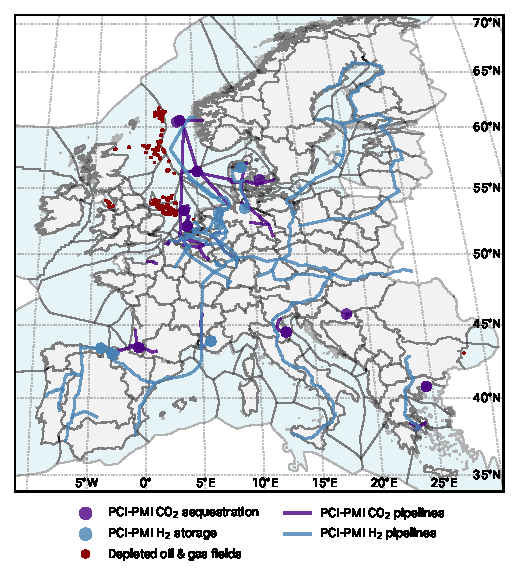
\includegraphics[width=0.8\linewidth]{map_adm_pcipmi}
  \caption{Map of the regional scope including clustered onshore (grey) and offshore regions (blue), as well as PCI-PMI \ce{CO2} and \ce{H2} pipelines, storage and sequestration sites. Depleted offshore oil and gas fields (red) provide additional \ce{CO2} sequestration potential \cite{hofmannH2CO2Network2025}.}
  \label{fig:regional_scope_map}
\end{figure}

Our implementation can adapt to the needs and configuration of the model, including selected technologies, geographical and temporal resolution, as well as the level of sector-coupling. Here, all projects are mapped to the 99 NUTS regions, in this process, pipelines are are aggregated and connect all overpassing regions. Similar to how all electricity lines and carrier links are modelled in PyPSA-Eur, lengths are calculated using the haversine formula multiplied by a factor of 1.25 to account for the non-straight shape of pipelines.
We apply standardised cost assumptions \cite{zeyenPyPSATechnologydataV01012025} across all existing brownfield assets, model-endogenously selected projects, and exogenously specified PCI-PMI projects, equally. Our approach is motivated by two key considerations: (i) cost data submitted by project promoters are often incomplete and may differ in terms of included components, underlying assumptions, and risk margins; and (ii) applying uniform cost assumptions ensures comparability and a level playing field across all potential investments, including both PCI-PMI and model-endogenous options. 

\paragraph{\ce{CO2} sequestration sites}
\label{sec:co2_sequestration_sites}
Beyond \ce{CO2} sequestration site projects included in the latest PCI-PMI list (around 114 Mt p.a.), we consider additional technical potential from the European \ce{CO2} storage database \cite{europeancommissionEuropeanCO2Storage2020,hofmannH2CO2Network2025}. While social and commercial acceptance of \ce{CO2} storage has been increasing in recent years, however, concerns still exist regarding its long-term purpose and safety \cite{vanalphenSocietalAcceptanceCarbon2007}. For this reason, we only consider conservative estimates from depleted oil and gas fields, which are primarily located offshore in the British, Norwegian, and Dutch North Sea (see Figure \ref{fig:regional_scope_map}), yielding a total sequestration potential of \SI{7164}{Mt}. Spread over a lifetime of 25 years, this translates into an annual sequestration potential of up to 286 Mt p.a. We then cluster all offshore potential within a buffer radius of \SI{50}{km} per offshore bus region in each modelled NUTS region and connect them through offshore \ce{CO2} pipelines to the closest onshore bus (TODO: add reference to cost assumptions in appendix). 


\subsection{Scenario setup and regret matrix}
\label{sec:scenario_setup}
To assess the long-term impact of PCI-PMI projects on the European energy system and EU energy policies, we implement a regret-matrix based approach. This allows us to evaluate the performance of a set of long-term scenarios under three different short-term occurrences for each planning horizon, individually (Table \ref{tab:regret_matrix_setup}).

\subsubsection{Long-term scenarios}
\paragraph{Scenario definition}
\label{sec:definition}
We define the long-term scenarios based on the degree of \ce{CO2} and \ce{H2} infrastructure build-out, including the roll-out of PCI-PMI projects as well additional pipeline investments. In total, we implement five long-term scenarios, (i) a pessimistic scenario (Decentral Islands --- DI) without any \ce{H2} pipeline and onshore \ce{CO2} pipeline infrastructure, (ii) a scenario that considers the on-time commissioning of all PCI-PMI \ce{CO2} and \ce{H2} projects (PCI-PMI --- PCI) only, (iii) more ambitious scenarios that further allow investments into national and (iv) international pipelines (PCI-PMI nat. --- PCI-n and PCI-PMI internat. --- PCI-in), and (v) a scenario that does not assume any fixed PCI-PMI infrastructure but allows for a centralised, purely needs-based build-out of \ce{CO2} and \ce{H2} pipelines (Centralised Planning --- CP). An overview of the long-term scenarios and their associated model-endogenous decision variables is provided in Table \ref{tab:long-term_scenarios}. 

\todo[inline]{Regarding Depleted oil and gas fields in table, TB: depleted fields is only one type of sequestration site - most is saline aquifers, oder? or are these PCI-PMI? is there any overlap between PCI-PMI sites and the depleted Oil and Gas? some details here would be useful}
\todo[inline]{Regarding endogenous H2 storage build-out, TB: does this respect salt deposit availability?}

\begin{table*}[htbp]
  \centering
  \caption{Overview of long-term scenarios and their key assumptions.}
  \label{tab:long-term_scenarios}
  \scriptsize
  \begin{tabularx}{\textwidth}{R{3.9cm}>{\centering\arraybackslash}X>{\centering\arraybackslash}X>{\centering\arraybackslash}X>{\centering\arraybackslash}X>{\centering\arraybackslash}X}
    \toprule
    \textbf{Long-term scenarios} & 
    \textbf{DI} & 
    \textbf{PCI} & 
    \textbf{PCI-n} & 
    \textbf{PCI-in} & 
    \textbf{CP} \\
    \midrule
    \textbf{\ce{CO2} sequestration} & & & & & \\
    Depleted oil \& gas fields* & $\blacksquare$ & $\blacksquare$ & $\blacksquare$ & $\blacksquare$ & $\blacksquare$ \\
    PCI-PMI seq. sites** & -- & $\blacksquare$ & $\blacksquare$ & $\blacksquare$ & $\blacksquare$ \\
    \midrule
    \textbf{\ce{H2} storage} & & & & & \\
    Endogenous build-out & $\blacksquare$ & $\blacksquare$ & $\blacksquare$ & $\blacksquare$ & $\blacksquare$ \\
    PCI-PMI storage sites & -- & $\blacksquare$ & $\blacksquare$ & $\blacksquare$ & $\blacksquare$ \\
    \midrule
    \textbf{\ce{CO2} pipelines} & & & & & \\
    to depleted oil \& gas fields & $\blacksquare$ & $\blacksquare$ & $\blacksquare$ & $\blacksquare$ & $\blacksquare$ \\
    to PCI-PMI seq. sites & -- & $\blacksquare$ & $\blacksquare$ & $\blacksquare$ & $\blacksquare$ \\
    \midrule
    \textbf{\ce{CO2} and \ce{H2} pipelines} & & & & & \\
    PCI-PMI & -- & $\blacksquare$ & $\blacksquare$ & $\blacksquare$ & $\blacksquare$ \\
    National build-out & -- & $\blacksquare$ & $\blacksquare$ & $\blacksquare$ & $\blacksquare$ \\
    International build-out & -- & -- & -- & $\blacksquare$ & $\blacksquare$ \\
    PCI-PMI extendable & -- & -- & -- & -- & $\blacksquare$ \\

    \bottomrule
  \end{tabularx}
  \caption*{\scriptsize $\blacksquare$ enabled \quad -- disabled \quad * approx. 286 Mt p.a. \quad ** approx. 114 Mt p.a.}
\end{table*}

\paragraph{Targets}
\label{sec:targets}
In all long-term scenarios, emission, technology, sequestration and production targets have to be met for each planning horizon (see Table \ref{tab:targets}). For the year 2030, these targets are directly derived from the EU's policy targets, including a \SI{55}{\percent} reduction in greenhouse gas emissions compared to 1990 levels \cite{europeancommissionFit55Delivering2021}, \SI{10}{Mt} p.a. of domestic green \ce{H2} production \cite{europeancommissionREPowerEUPlanCommunication2022} and \SI{40}{GW} of electrolyser capacity \cite{europeancommissionCommunicationCommissionEuropean2020}, and \SI{50}{Mt} p.a. of \ce{CO2} sequestration capacity \cite{europeanparliamentRegulationEU20242024}. For 2050, the \ce{CO2} are based on the modelling the impact assessment for the EU's 2040 climate targets, in 250 Mt p.a. need to be sequestered \cite{europeancommissionCommunicationCommissionEuropean2024}. \ce{H2} production targets for 2050 are based on the European Commission's METIS 3 study S5 \cite{europeancommission.directorategeneralforenergy.METIS3Study2023}, modelling possible pathways for industry decarbonisation until 2040. For 2040, we interpolate linearly between the 2030 and 2050 targets. The electrolyser capacities for 2040 and 2050 are scaled by the ratio of \ce{H2} production to electrolyser capacity in 2030. An overview of the targets and their values is provided in Table \ref{tab:targets}. Note that we implement the green \ce{H2 production} target as a minimum \ce{H2} production constraint from electrolysis
, hence we will refer to this \ce{H2} as electrolytic \ce{H2} within the scope of this paper.

\begin{table*}[htbp]
  \centering
  \caption{Pathway for implemented targets.}
  \label{tab:targets}
  \scriptsize
  \begin{tabularx}{\textwidth}{R{3.9cm}>{\centering\arraybackslash}X>{\centering\arraybackslash}X>{\centering\arraybackslash}X}
    \toprule
    \textbf{Planning horizon} & \textbf{2030} & \textbf{2040} & \textbf{2050} \\
    \midrule
    \textbf{Targets} & & & \\
    GHG emission reduction &  \SI{-55}{\percent} & \SI{-90}{\percent} & \SI{-100}{\percent} \\
    \ce{CO2} sequestration & 50 Mt p.a. & 150 Mt p.a. & 250 Mt p.a. \\
    Electrolytic \ce{H2} production & 10 Mt p.a. & 27.5 Mt p.a. & 45 Mt p.a. \\
    \ce{H2} electrolyser capacity & \SI{40}{GW} &  \SI{110}{GW} &  \SI{180}{GW} \\
    \bottomrule
  \end{tabularx}
  \caption*{\scriptsize Model targets based on \cite{europeancommissionFit55Delivering2021,europeancommissionREPowerEUPlanCommunication2022,europeanparliamentRegulationEU20242024,europeancommissionCommunicationCommissionEuropean2024,europeancommission.directorategeneralforenergy.METIS3Study2023}}
\end{table*}

\subsubsection{Short-term scenarios}
\label{sec:short-term_scenarios}
In a second step, we assess the impact of three short-term scenarios on the long-term scenarios, i.e., the \ce{CO2} and \ce{H2} pipeline capacities built in the long-term scenarios are either frozen or removed. Further, the model can still react by investing into additional generation, storage, or conversion, or carbon-removal technologies in the short-term, assuming the technical potential was not exceeded in the long-term optimisation. In \textit{Reduced targets}, we remove all of the long-term targets (Table \ref{tab:targets}) except for the GHG emission reduction targets to assess the value of the \ce{CO2} and \ce{H2} infrastructure in a less ambitious policy environment \cite{europeancourtofauditorsEUsIndustrialPolicy2024}. In \textit{Delayed pipelines}, we assume that all PCI-PMI and endogenous pipelines are delayed by one period, i.e., the commissioning of the project is shifted to the next planning horizon. Lastly, we remove all pipeline capacities in \textit{No pipelines}, including the PCI-PMI projects, allowing us to evaluate the impact of a complete lack of planned infrastructure. 

Table \ref{tab:regret_matrix_setup} gives an overview of this regret-analysis and their individual assumptions, where the long-term scenario serves as the \textit{planned} or \textit{anticipated} and the short-term scenario serves as the hypothetically \textit{realised} outcome. A regret matrix provides a decision-making framework that evaluates the potential loss (\textit{regret}) associated with choosing one strategy over the other by comparing the outcomes, i.e., the total system costs. Here, the regret is quantified as the difference between system costs of the short-term scenario and the long-term (anticipated) scenario for each scenario. 
In total, we run 60 optimisations on a cluster, taking up to 160 GB of RAM and 8 to 16 hours each to solve: ($n_{LT} \times n_{planning\,horizons}) \times (1+n_{ST}) = 60$. The models are solved using Gurobi.

\begin{table*}[htbp]
  \centering
  \caption{Regret matrix setup: Long-term and short-term scenarios.}
  \label{tab:regret_matrix_setup}
  \scriptsize
  \begin{tabularx}{\textwidth}{R{3.9cm}>{\centering\arraybackslash}X>{\centering\arraybackslash}X>{\centering\arraybackslash}X}
    \toprule
    \textbf{Short-term} & \textbf{Reduced targets} & \textbf{Delayed pipelines} & \textbf{No pipelines} \\
    \midrule
    \textbf{Long-term scenarios} & & & \\
    Decentral Islands (\textbf{DI}) & $\blacksquare$ & -- & -- \\
    PCI-PMI (\textbf{PCI}) & $\blacksquare$ & $\blacksquare$ & $\blacksquare$ \\
    PCI-PMI nat. (\textbf{PCI-n}) & $\blacksquare$ & $\blacksquare$ & $\blacksquare$\\
    PCI-PMI internat. (\textbf{PCI-in}) & $\blacksquare$ & $\blacksquare$ & $\blacksquare$ \\
    Central Planning (\textbf{CP}) & $\blacksquare$ & $\blacksquare$ & $\blacksquare$ \\
    \midrule
    \textbf{Targets} & & & \\
    GHG emission reduction &  $\blacksquare$ &  $\blacksquare$ &  $\blacksquare$ \\
    \ce{CO2} sequestration &  -- &  $\blacksquare$ &  $\blacksquare$ \\
    Electrolytic \ce{H2} production &  -- &  $\blacksquare$ &  $\blacksquare$ \\
    \ce{H2} electrolysers &  -- &  $\blacksquare$ &  $\blacksquare$ \\
    \midrule
    \textbf{\ce{CO2} + \ce{H2} infrastructure} & & & \\
    \ce{CO2} sequestration sites & $\blacksquare$ &  $\blacksquare$ &  $\blacksquare$ \\
    \ce{CO2} pipelines to seq. site & $\blacksquare$ &  $\blacksquare$ &  $\blacksquare$ \\
    \ce{CO2} pipelines & $\blacksquare$ &  $\square$ &  -- \\
    \ce{H2} pipelines & $\blacksquare$ &  $\square$ &  -- \\
    \bottomrule
  \end{tabularx}
  \caption*{\scriptsize $\blacksquare$ enabled \quad $\square$ delayed by one period \quad -- disabled}
\end{table*}

\section{Results and discussion}
\label{sec:results_and_discussion}
We structure the results and discussion into three main sections. First, we present the results of the long-term scenarios. Then, we look at the impact of the short-term scenarios on the long-term scenarios, by comparing the economic regret and impacts on \ce{CO2} and \ce{H2 balances}. Finally, we assess the benefits of the PCI-PMI projects with regard to reduced system costs and discuss the implications of our findings for the European energy system and its policy targets. 

\subsection{Long-term scenarios}
\label{sec:long-term_scenarios}
In all long-term runs, we observe the highest total annual system costs in the planning horizon 2040, ranging from 912 to 968 bn. \euro{} p.a. (Figure \ref{fig:costs_overview}), driven by high investments. This can be primarily attributed to the strict exogenously given GHG emission reduction pathway, facing the largest net change from 2030 to 2040 --- a carbon budget reduction of more than 1600 Mt p.a. as opposed to the remaining 460 Mt p.a. in the last decade. In 2030, total system costs are lowest in the \textit{DI} and \textit{CP} scenario, as the model does not see the need for large-scale investments into \ce{H2} and \ce{CO2} infrastructure yet. With \ce{CO2} pipelines connecting depleted offshore oil and gas fields to their closest onshore region, the policy targets, incl. \ce{CO2} sequestration can be achieved at a total of 865 bn. \euro{} p.a. Adding PCI-PMI projects in 2030 increases costs by less than \SI{1}{\percent}. 

\begin{figure}[htbp]
  \centering
  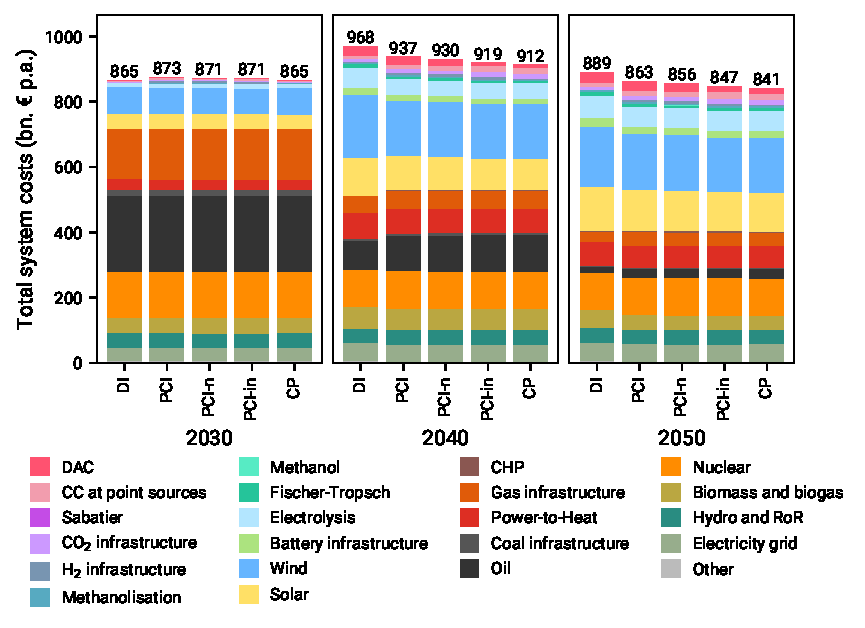
\includegraphics[width=\linewidth]{costs_overview.pdf}
  \caption{Total annual system costs (CAPEX + OPEX) by technology group.}
  \label{fig:costs_overview}
\end{figure}

Starting in 2040, all scenarios with PCI-PMI and endogenous pipeline investments unlock significant cost savings, from more than 30 bn. \euro{} p.a. in the \textit{PCI} up to 50 bn. \euro{} p.a. in the \textit{PCI-in} scenario. By giving the model complete freedom in pipeline expansions, additional annual cost savings of 6 to 7 bn. \euro{} are unlocked by investing in fewer, but more optimally located \ce{CO2} and \ce{H2} pipelines from a systemic perspective (see \textit{PCI-in} pipeline utilisation in Figures \ref{fig:PCI-in_lt_2030} to \ref{fig:PCI-in_lt_2050} compared to \textit{CP} pipeline utilisation in Figures \ref{fig:CP_lt_2030} to \ref{fig:CP_lt_2050}). Further, this reduces the reliance on larger investments into wind generation and more expensive Direct Air Capture (DAC) technologies near the sequestration sites. These effects are slightly less pronounced in the 2050 model results, system costs can be reduced by 26 to 41 bn. \euro{} p.a. with PCI-PMI and endogenous pipeline investments. 
\todo[inline]{TB: why? perhaps more CCU and FT and H2 makes system more flexible}

\begin{figure*}[htbp]
  \centering
  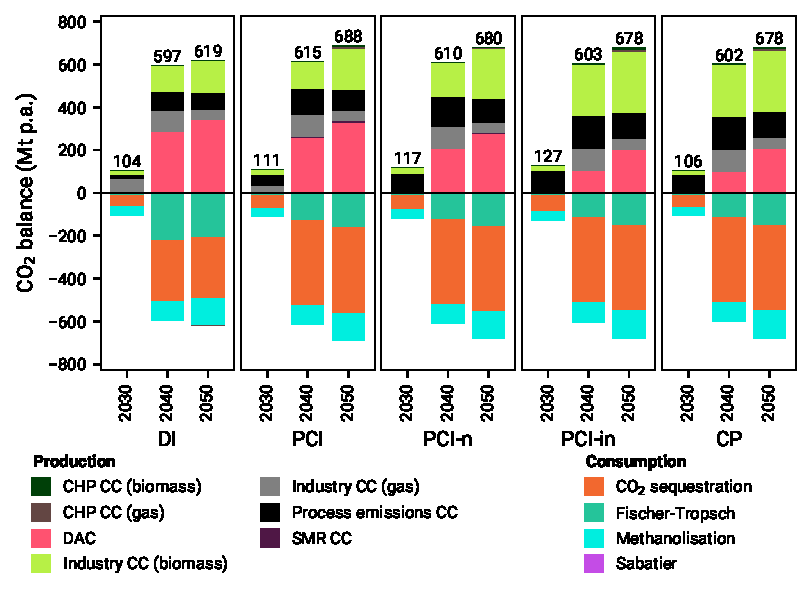
\includegraphics[width=\textwidth]{balances_overview_co2 stored}
  \caption{\ce{CO2} balances in long-term scenarios.}
  \label{fig:balances_overview_co2_stored}
\end{figure*}

\paragraph{Carbon capture, utilisation, and storage}
\label{sec:ccus}
We find that most of the differences in system cost and savings can be attributed to the production and utilisation of \ce{CO2}, as shown in Figure \ref{fig:balances_overview_co2_stored}. Lacking the option to transport \ce{CO2} from industry and other point sources to the offshore sequestration sites, the model has to invest in expensive DAC technologies in the \textit{DI} scenario. While the sequestration target of 50 Mt p.a. in 2030 is binding for the \textit{DI} scenario, all other scenarios sequester more \ce{CO2}, the higher their \ce{CO2} pipeline build-out. The 53.9 Mt p.a. \ce{CO2} sequestered in the \textit{CP} serve as an indicator for what would be a cost-optimal amount for 2030 with perfectly located pipelines. With the inclusion of PCI-PMI projects, \ce{CO2} sequestration ranges from 58.7 Mt p.a. in the \textit{PCI} to 75 Mt p.a. in the \textit{PCI-in} scenario. 
Looking at 2040 and 2050, in place of expensive DAC in the \textit{DI} scenario, the model equips biomass-based industrial processes primarily located in Belgium, the Netherlands and Western regions of Germany (see Figures \ref{fig:PCI_lt_2030_co2}, \ref{fig:PCI_lt_2040_co2}, and \ref{fig:PCI_lt_2050_co2}). 

In 2040 and 2050, all sequestration targets (Table \ref{tab:targets}) are overachieved, as the full combined \ce{CO2} sequestration potential of 398 Mt p.a. is exploited in all scenarios where PCI-PMI projects are included (\textit{PCI} to \textit{CP}). Emissions are captured from industrial processes equipped with carbon capture units, with biomass-based industry providing the largest share in carbon capture from point sources, ranging from 119 to 241 Mt p.a. in 2040 and 149 to 287 Mt p.a. in 2050, increasing with the build-out of \ce{CO2} infrastructure (from left to right, see Figure \ref{fig:balances_overview_co2_stored}). Being the most expensive carbon capture option, only up to 8 Mt p.a. of \ce{CO2} is captured from SMR CC processes in the \textit{PCI} scenario in 2050. 
With a lower sequestration potential of 286 Mt p.a. in \textit{DI} scenario, more \ce{CO2} is used as a precursor for the synthesis of Fischer-Tropsch fuels instead --- 221 Mt p.a. vs. 115-127 Mt p.a. (2040) and 206 Mt p.a. vs 153-163 Mt p.a. (2050), to meet the emission reduction targets for 2040 and 2050, respectively. 
Given the fixed exogenous demand for (shipping) methanol (Figure \ref{fig:exogenous_demand}), \ce{CO2} demand for methanolisation is constant across all scenarios (39 Mt p.a. in 2030, 89 Mt p.a. in 2040, and 127 Mt p.a. in 2050). 

\clearpage
\begin{figure*}[htbp]
  \centering
  \begin{subfigure}[t]{0.4\textwidth}
      \vspace{0pt}
      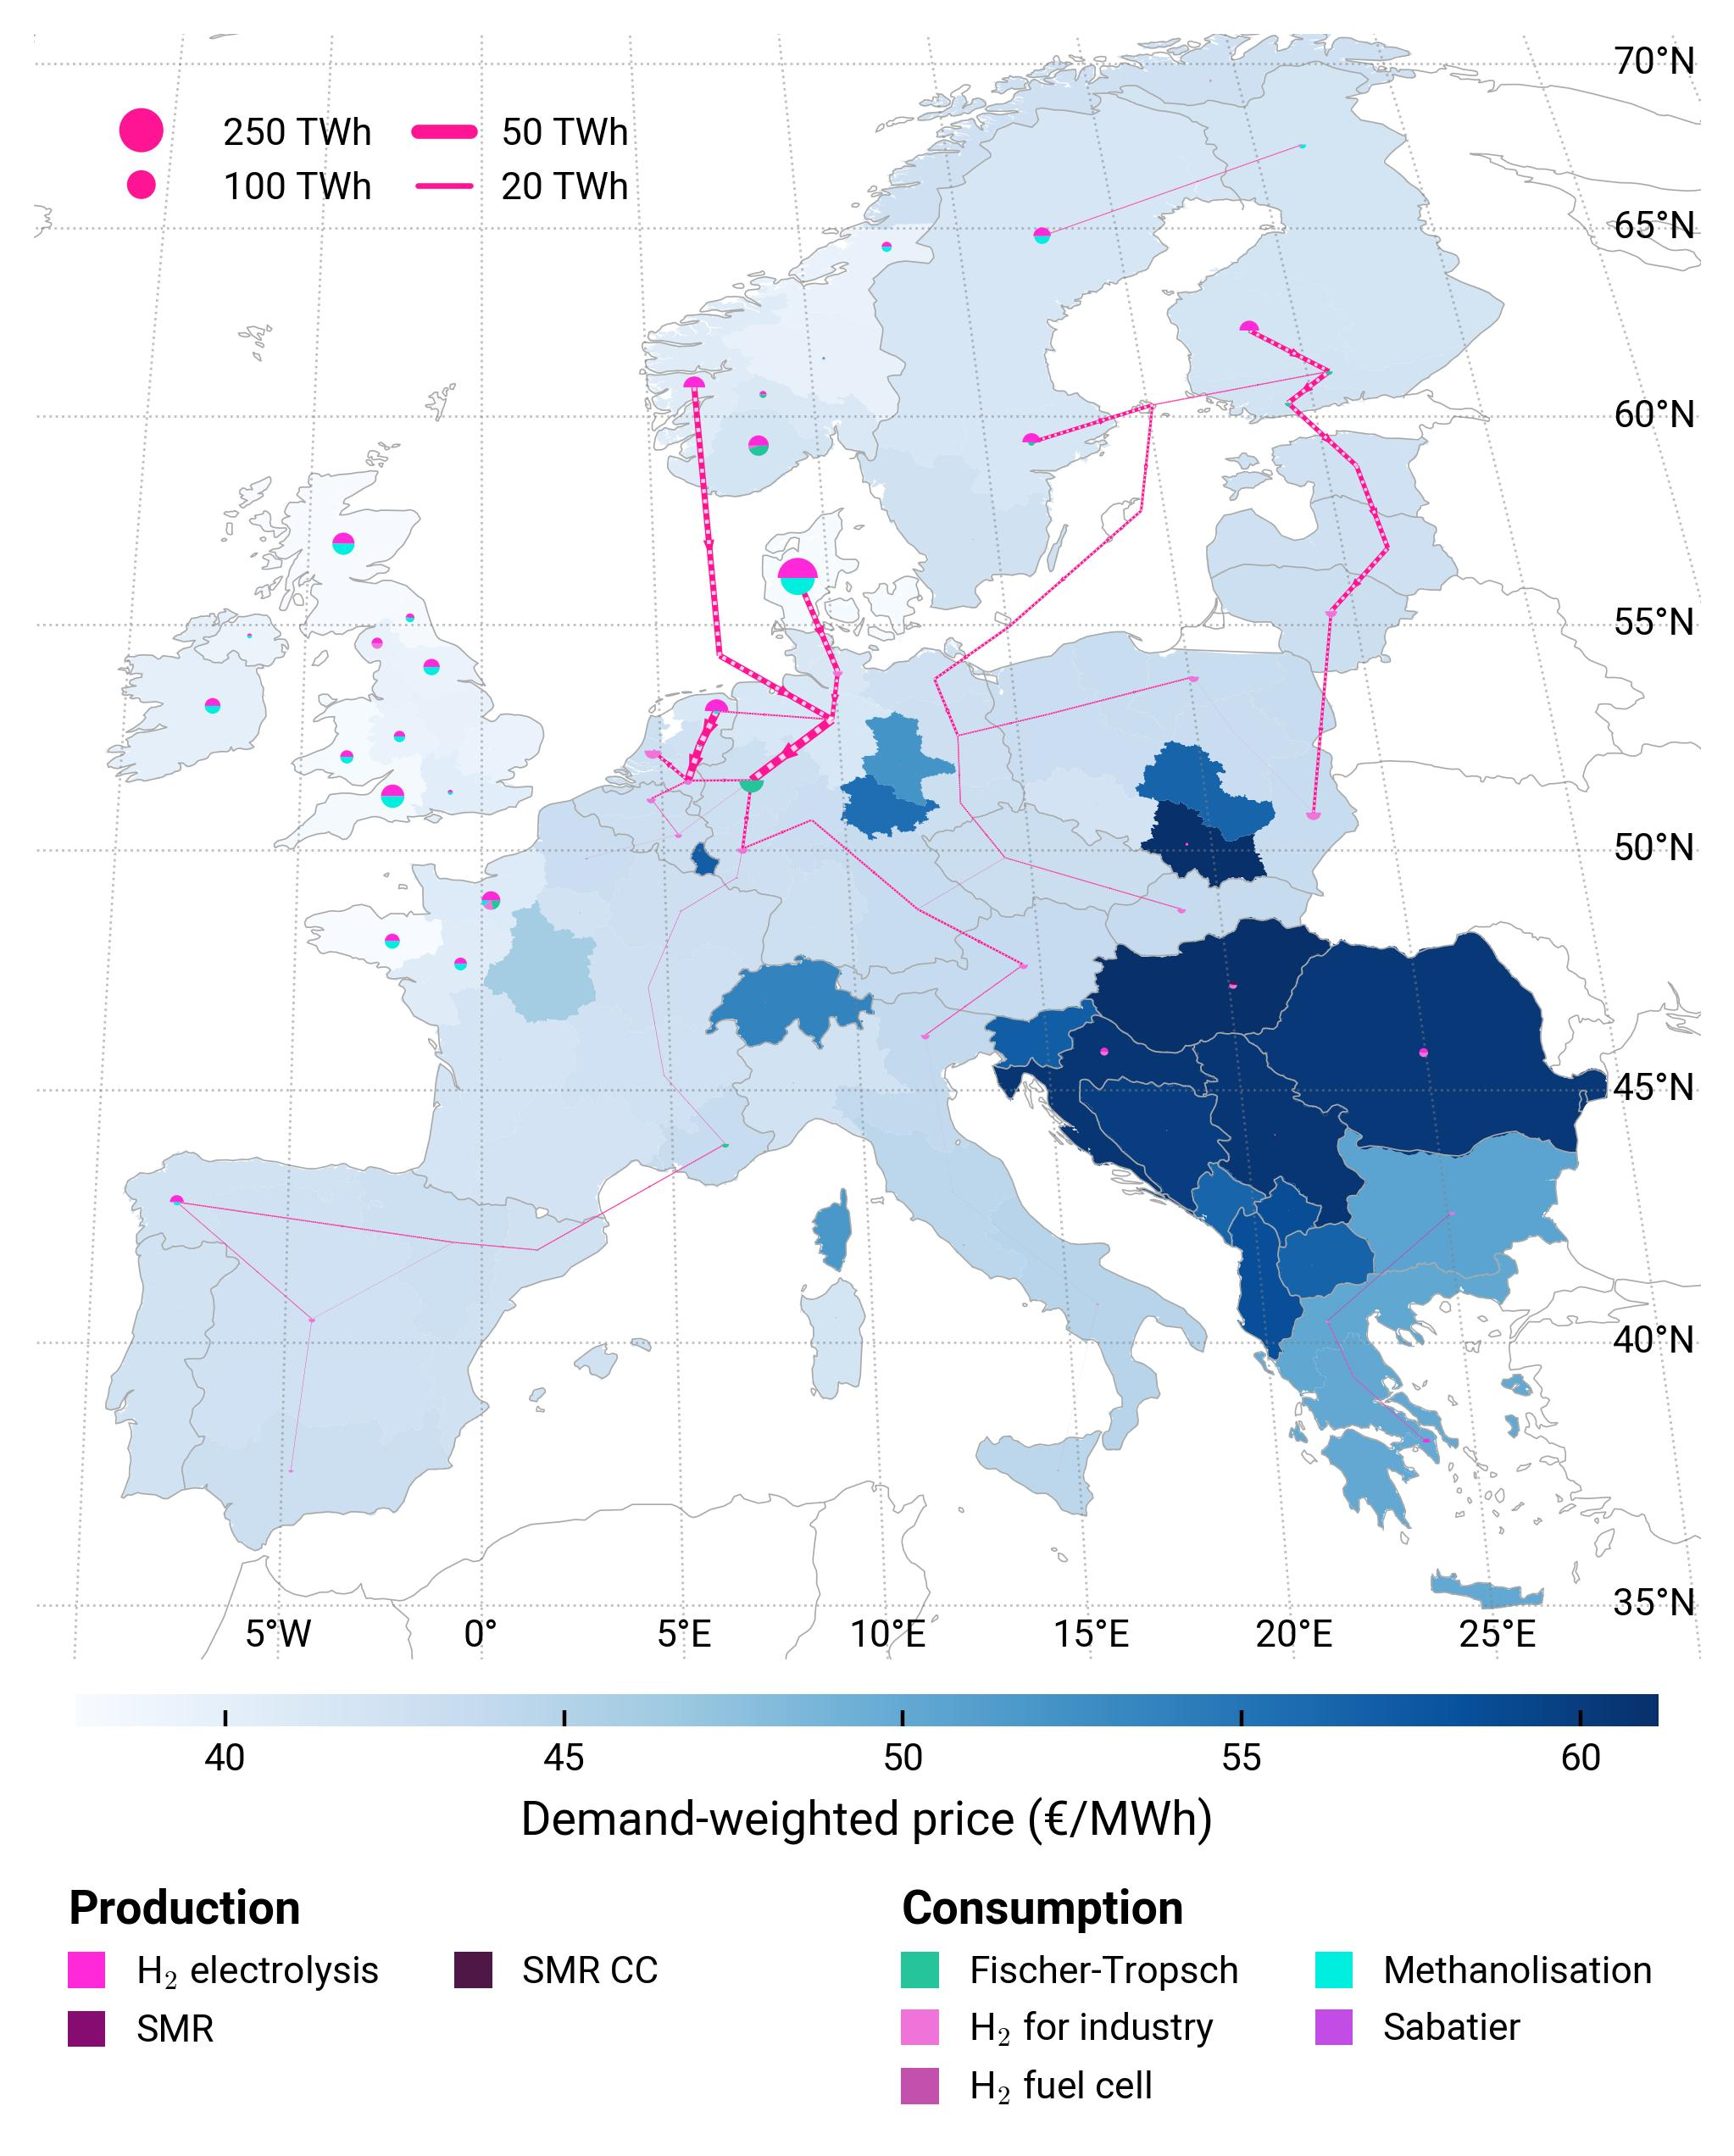
\includegraphics[width=1\textwidth,trim=0cm 2.8cm 0cm 0cm, clip]{maps/pcipmi/base_s_adm___2030-balance_map_H2}
      \vspace{-0.5cm}
      \caption{\ce{H2} 2030.}
      \label{fig:PCI_lt_2030_h2}
  \end{subfigure}
  \hfill
  \begin{subfigure}[t]{0.4\textwidth}
      \vspace{0pt}
      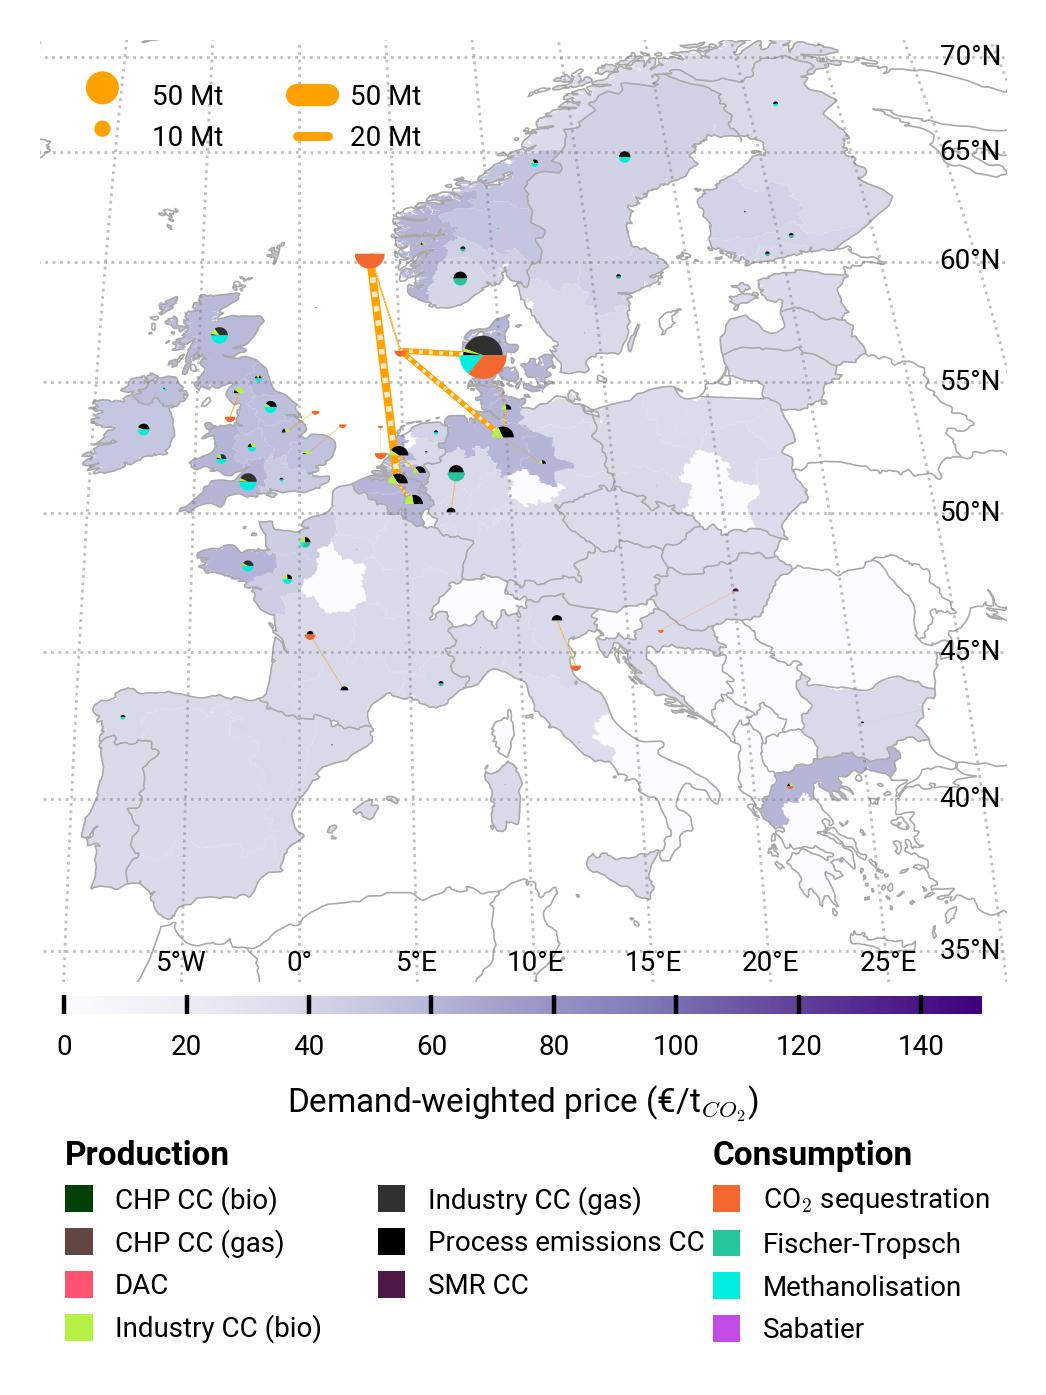
\includegraphics[width=1\textwidth,trim=0cm 3.2cm 0cm 0cm, clip]{maps/pcipmi/base_s_adm___2030-balance_map_co2_stored} 
      \vspace{-0.5cm}
      \caption{\ce{CO2} 2030.}
      \label{fig:PCI_lt_2030_co2}
  \end{subfigure}
  \begin{subfigure}[t]{0.4\textwidth}
      \vspace{0pt}
      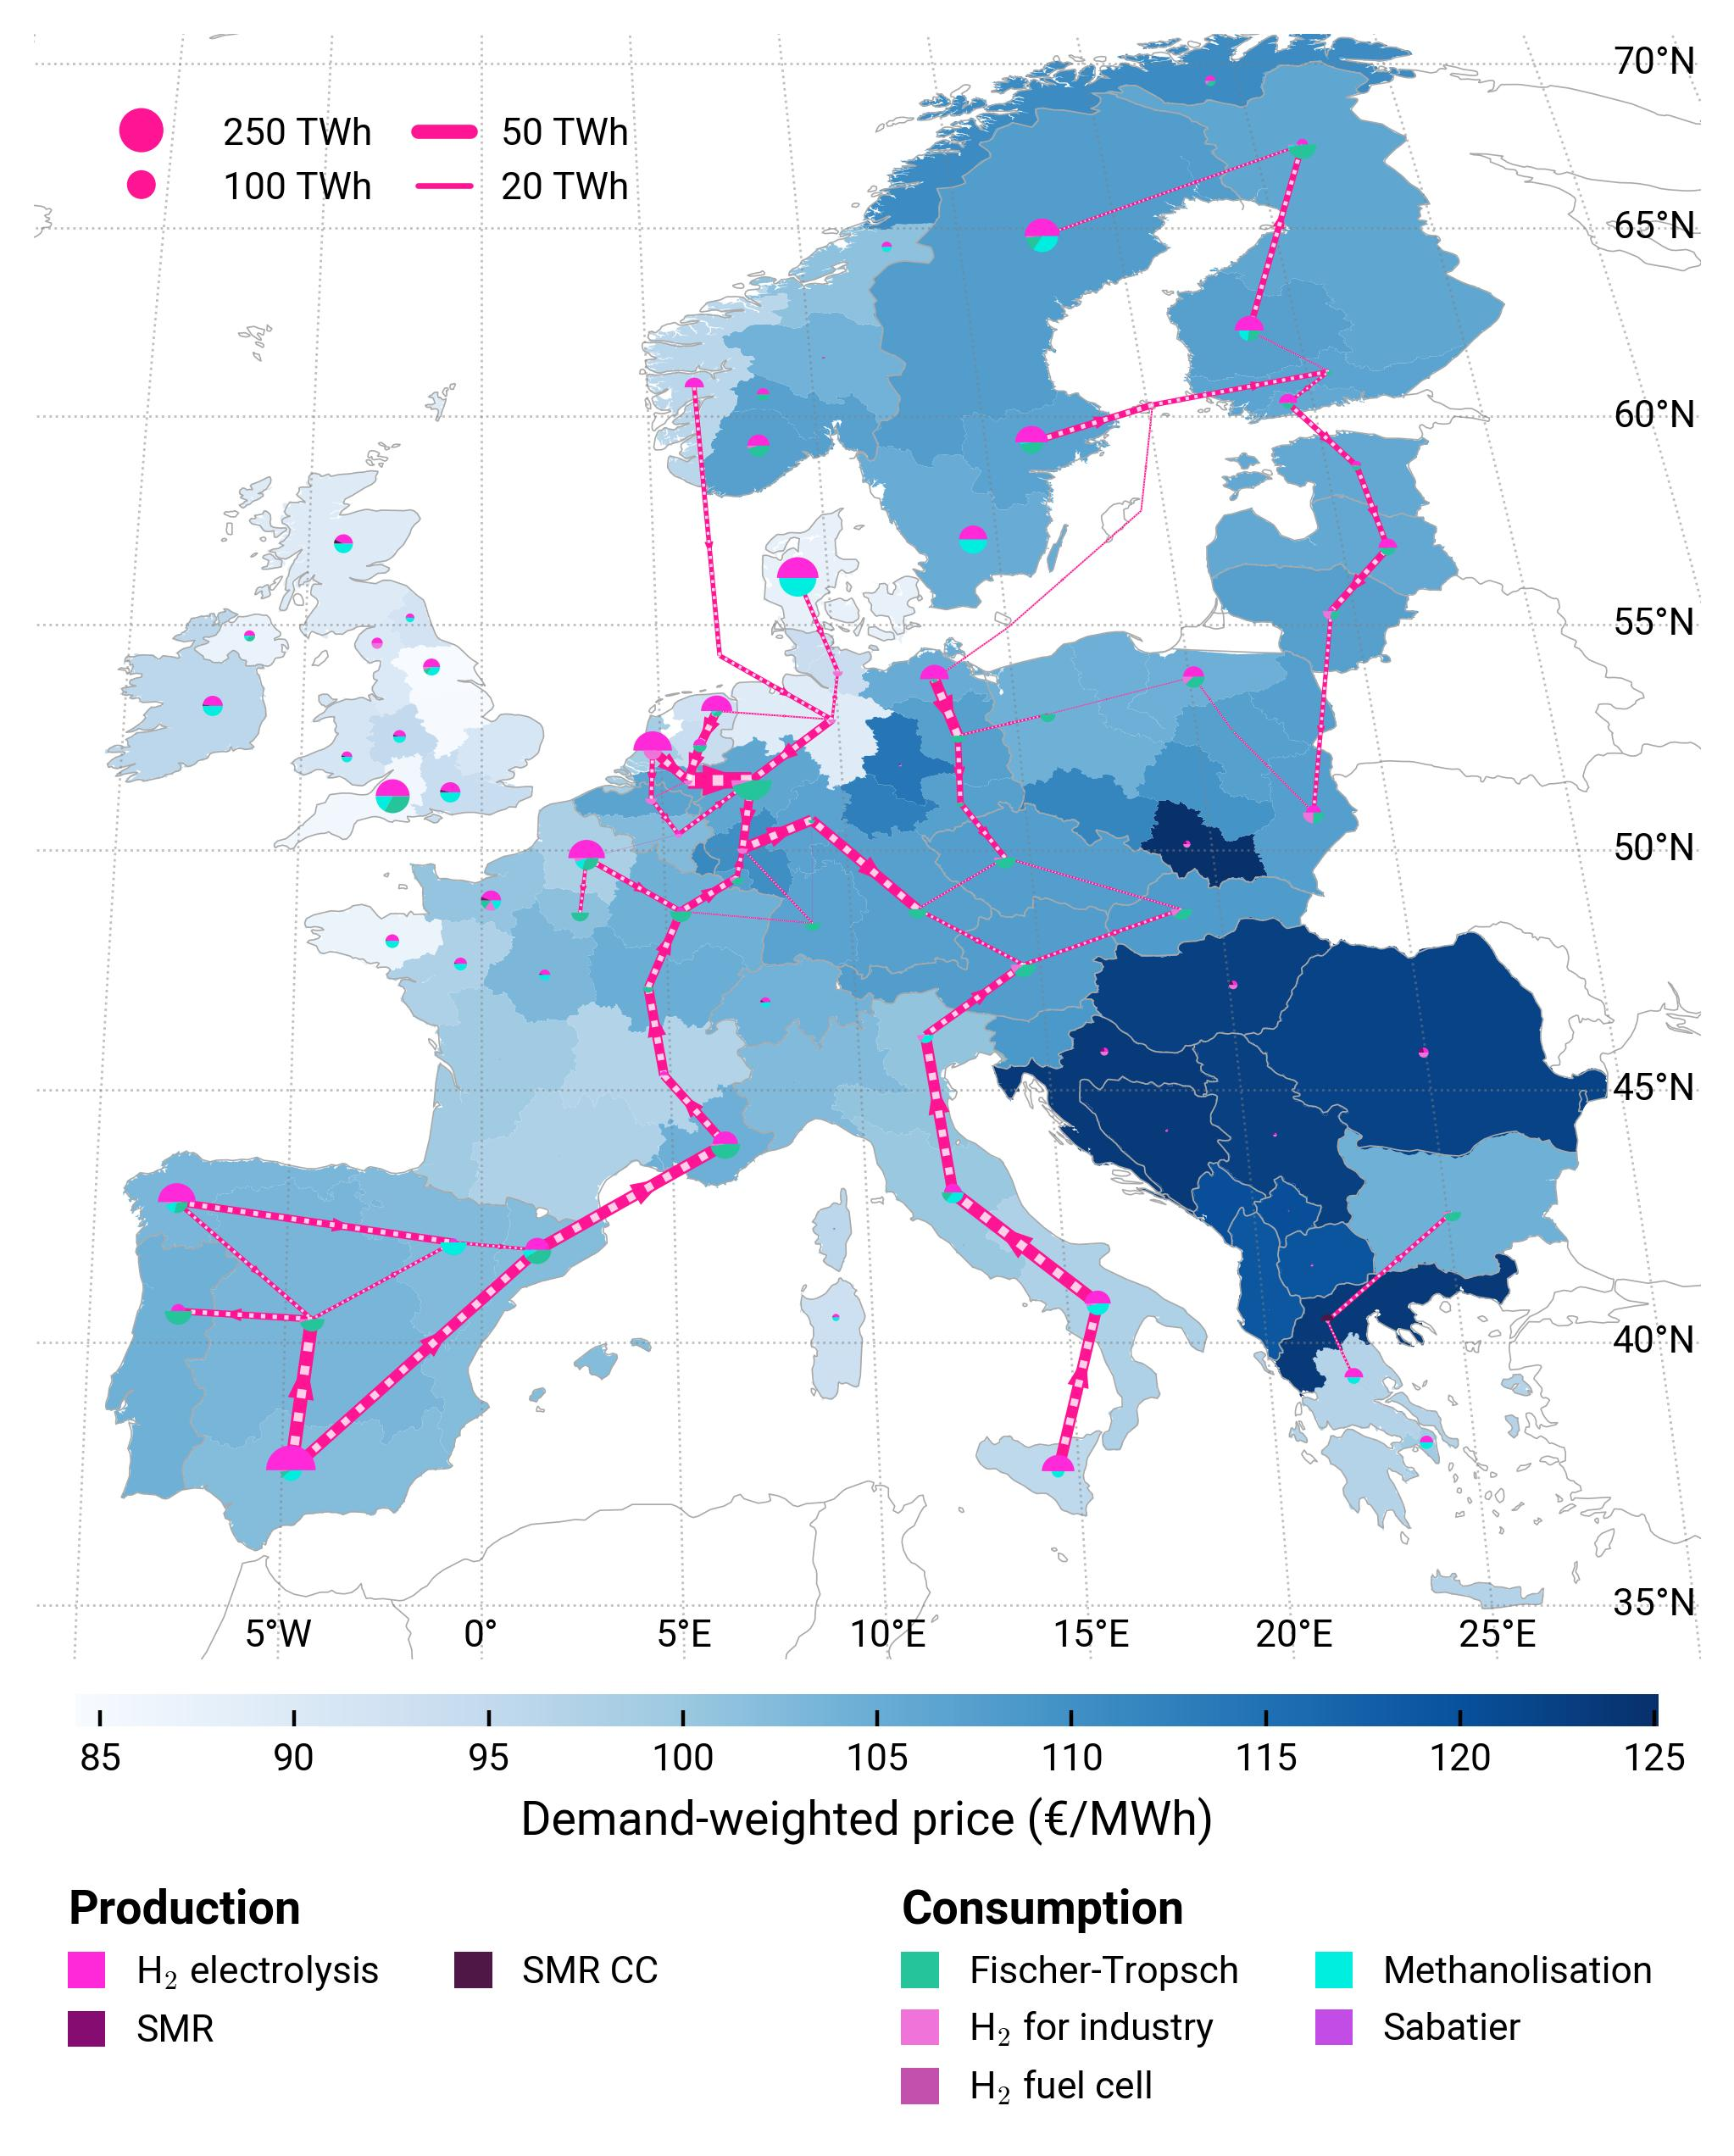
\includegraphics[width=1\textwidth,trim=0cm 2.8cm 0cm 0cm, clip]{maps/pcipmi/base_s_adm___2040-balance_map_H2}
      \vspace{-0.5cm}
      \caption{\ce{H2} 2040.}
      \label{fig:PCI_lt_2040_h2}
  \end{subfigure}
  \hfill
  \begin{subfigure}[t]{0.4\textwidth}
      \vspace{0pt}
      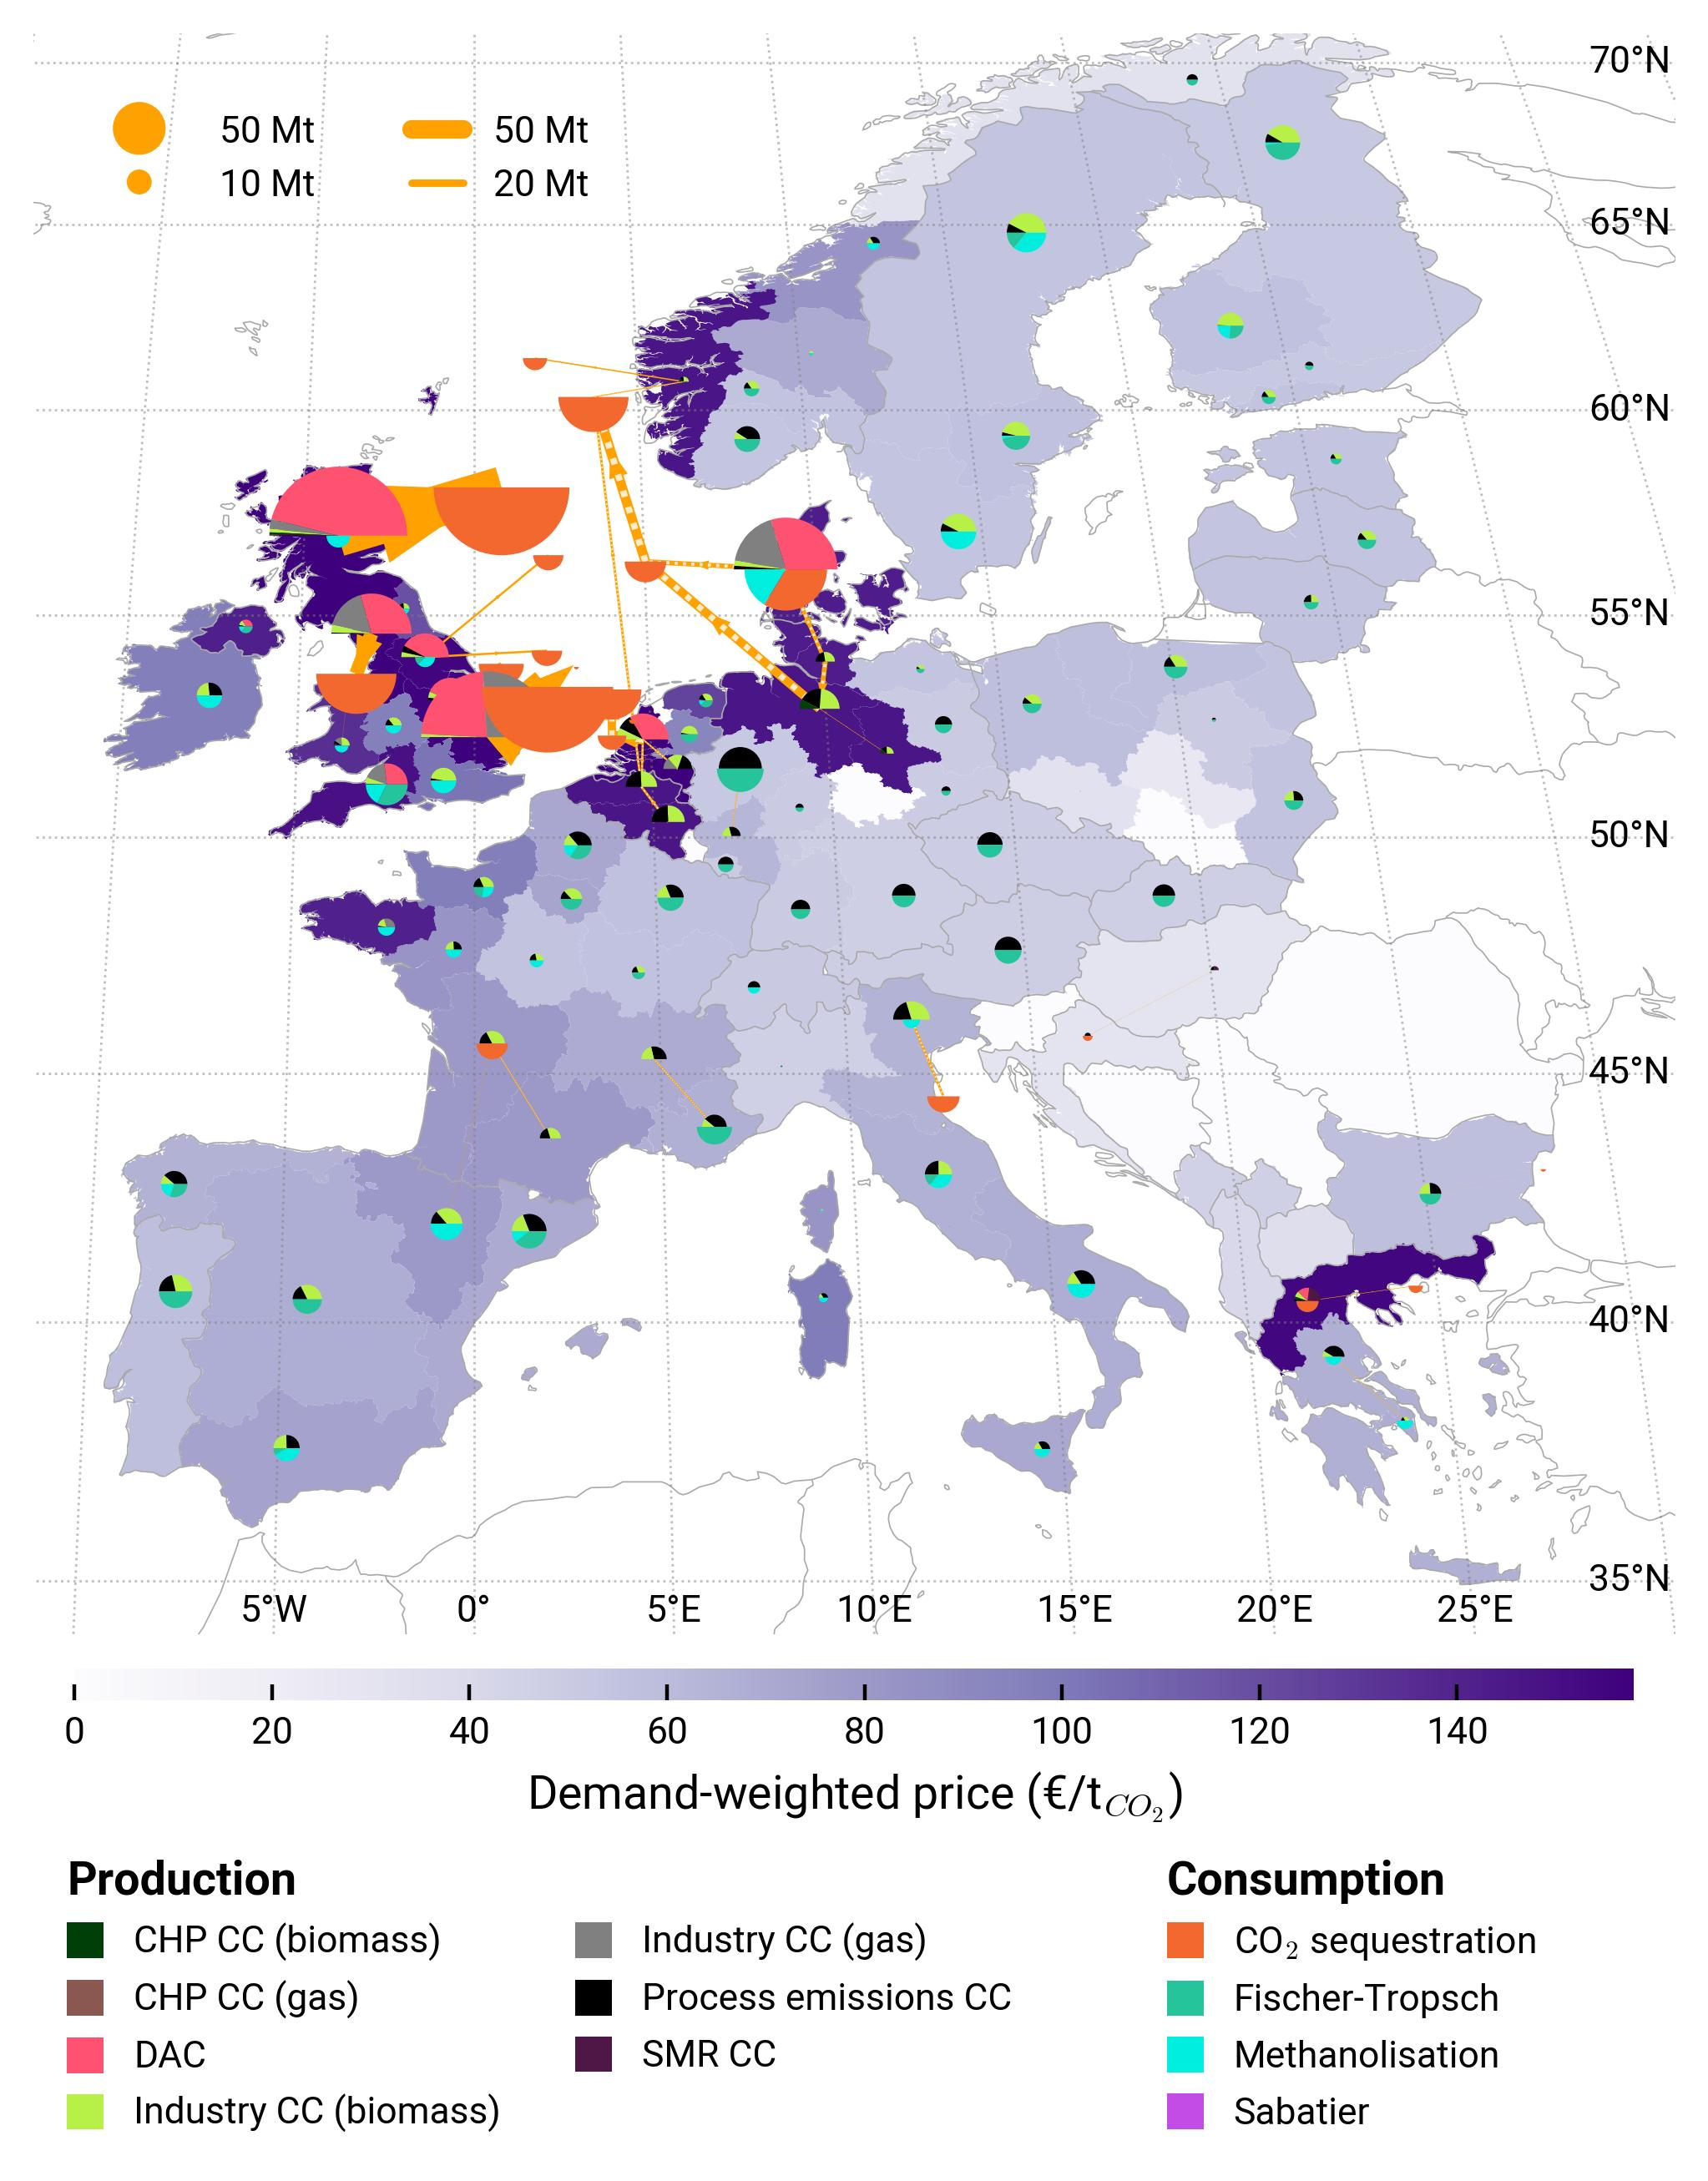
\includegraphics[width=1\textwidth,trim=0cm 3.2cm 0cm 0cm, clip]{maps/pcipmi/base_s_adm___2040-balance_map_co2_stored} 
      \vspace{-0.5cm}
      \caption{\ce{CO2} 2040.}
      \label{fig:PCI_lt_2040_co2}
  \end{subfigure}
  \begin{subfigure}[t]{0.4\textwidth}
      \vspace{0pt}
      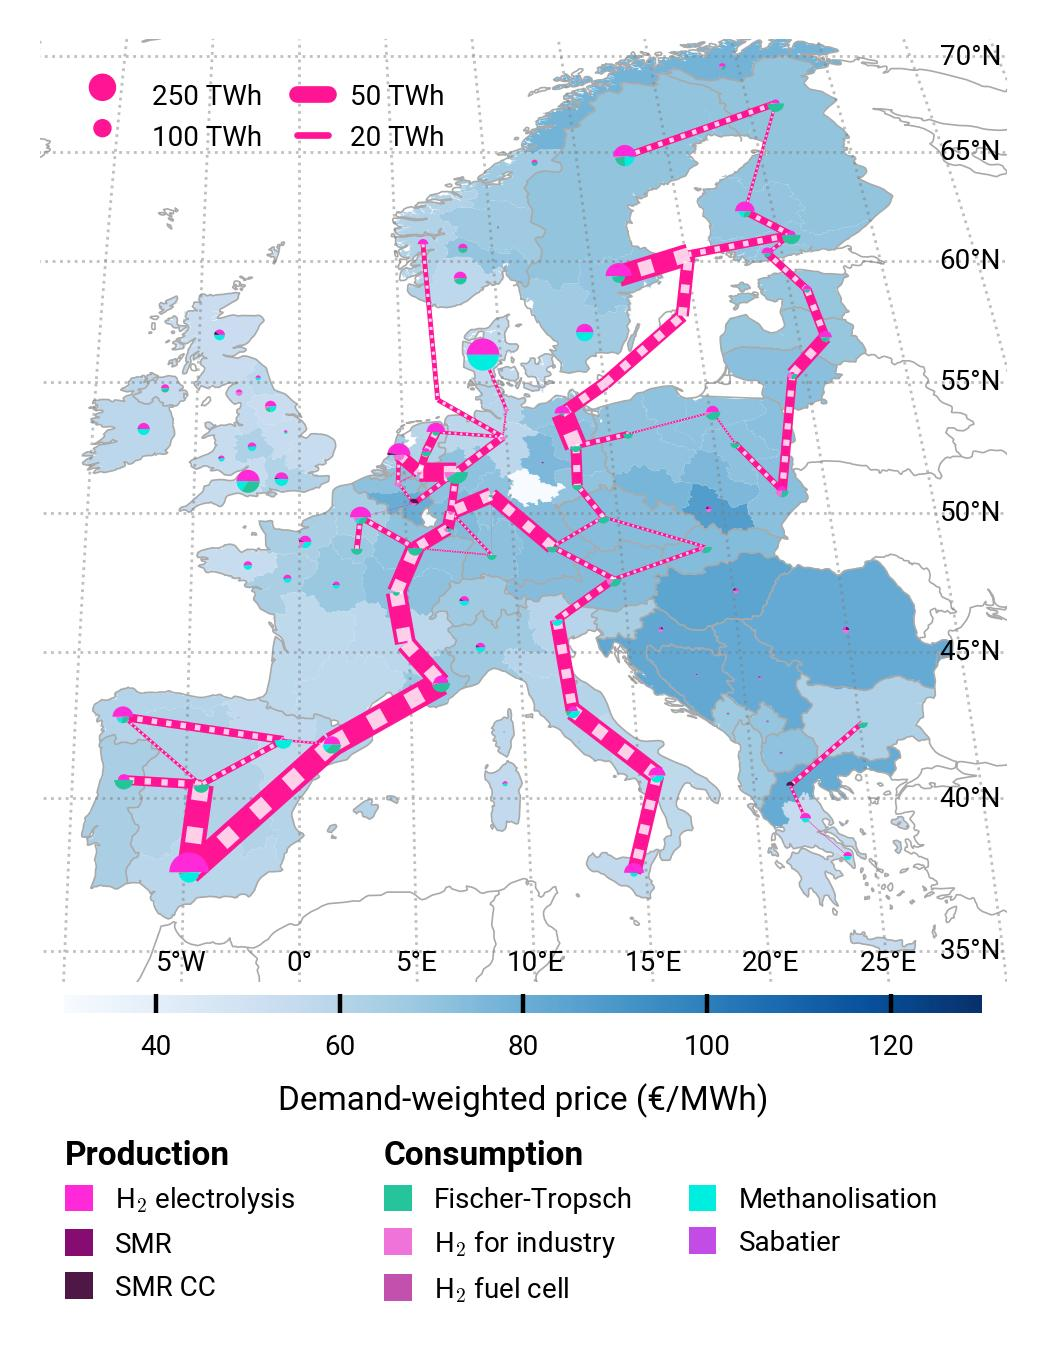
\includegraphics[width=1\textwidth,trim=0cm 0cm 0cm 0cm, clip]{maps/pcipmi/base_s_adm___2050-balance_map_H2}
      \vspace{-0.5cm}
      \caption{\ce{H2} 2050.}
      \label{fig:PCI_lt_2050_h2}
  \end{subfigure}
  \hfill
  \begin{subfigure}[t]{0.4\textwidth}
      \vspace{0pt}
      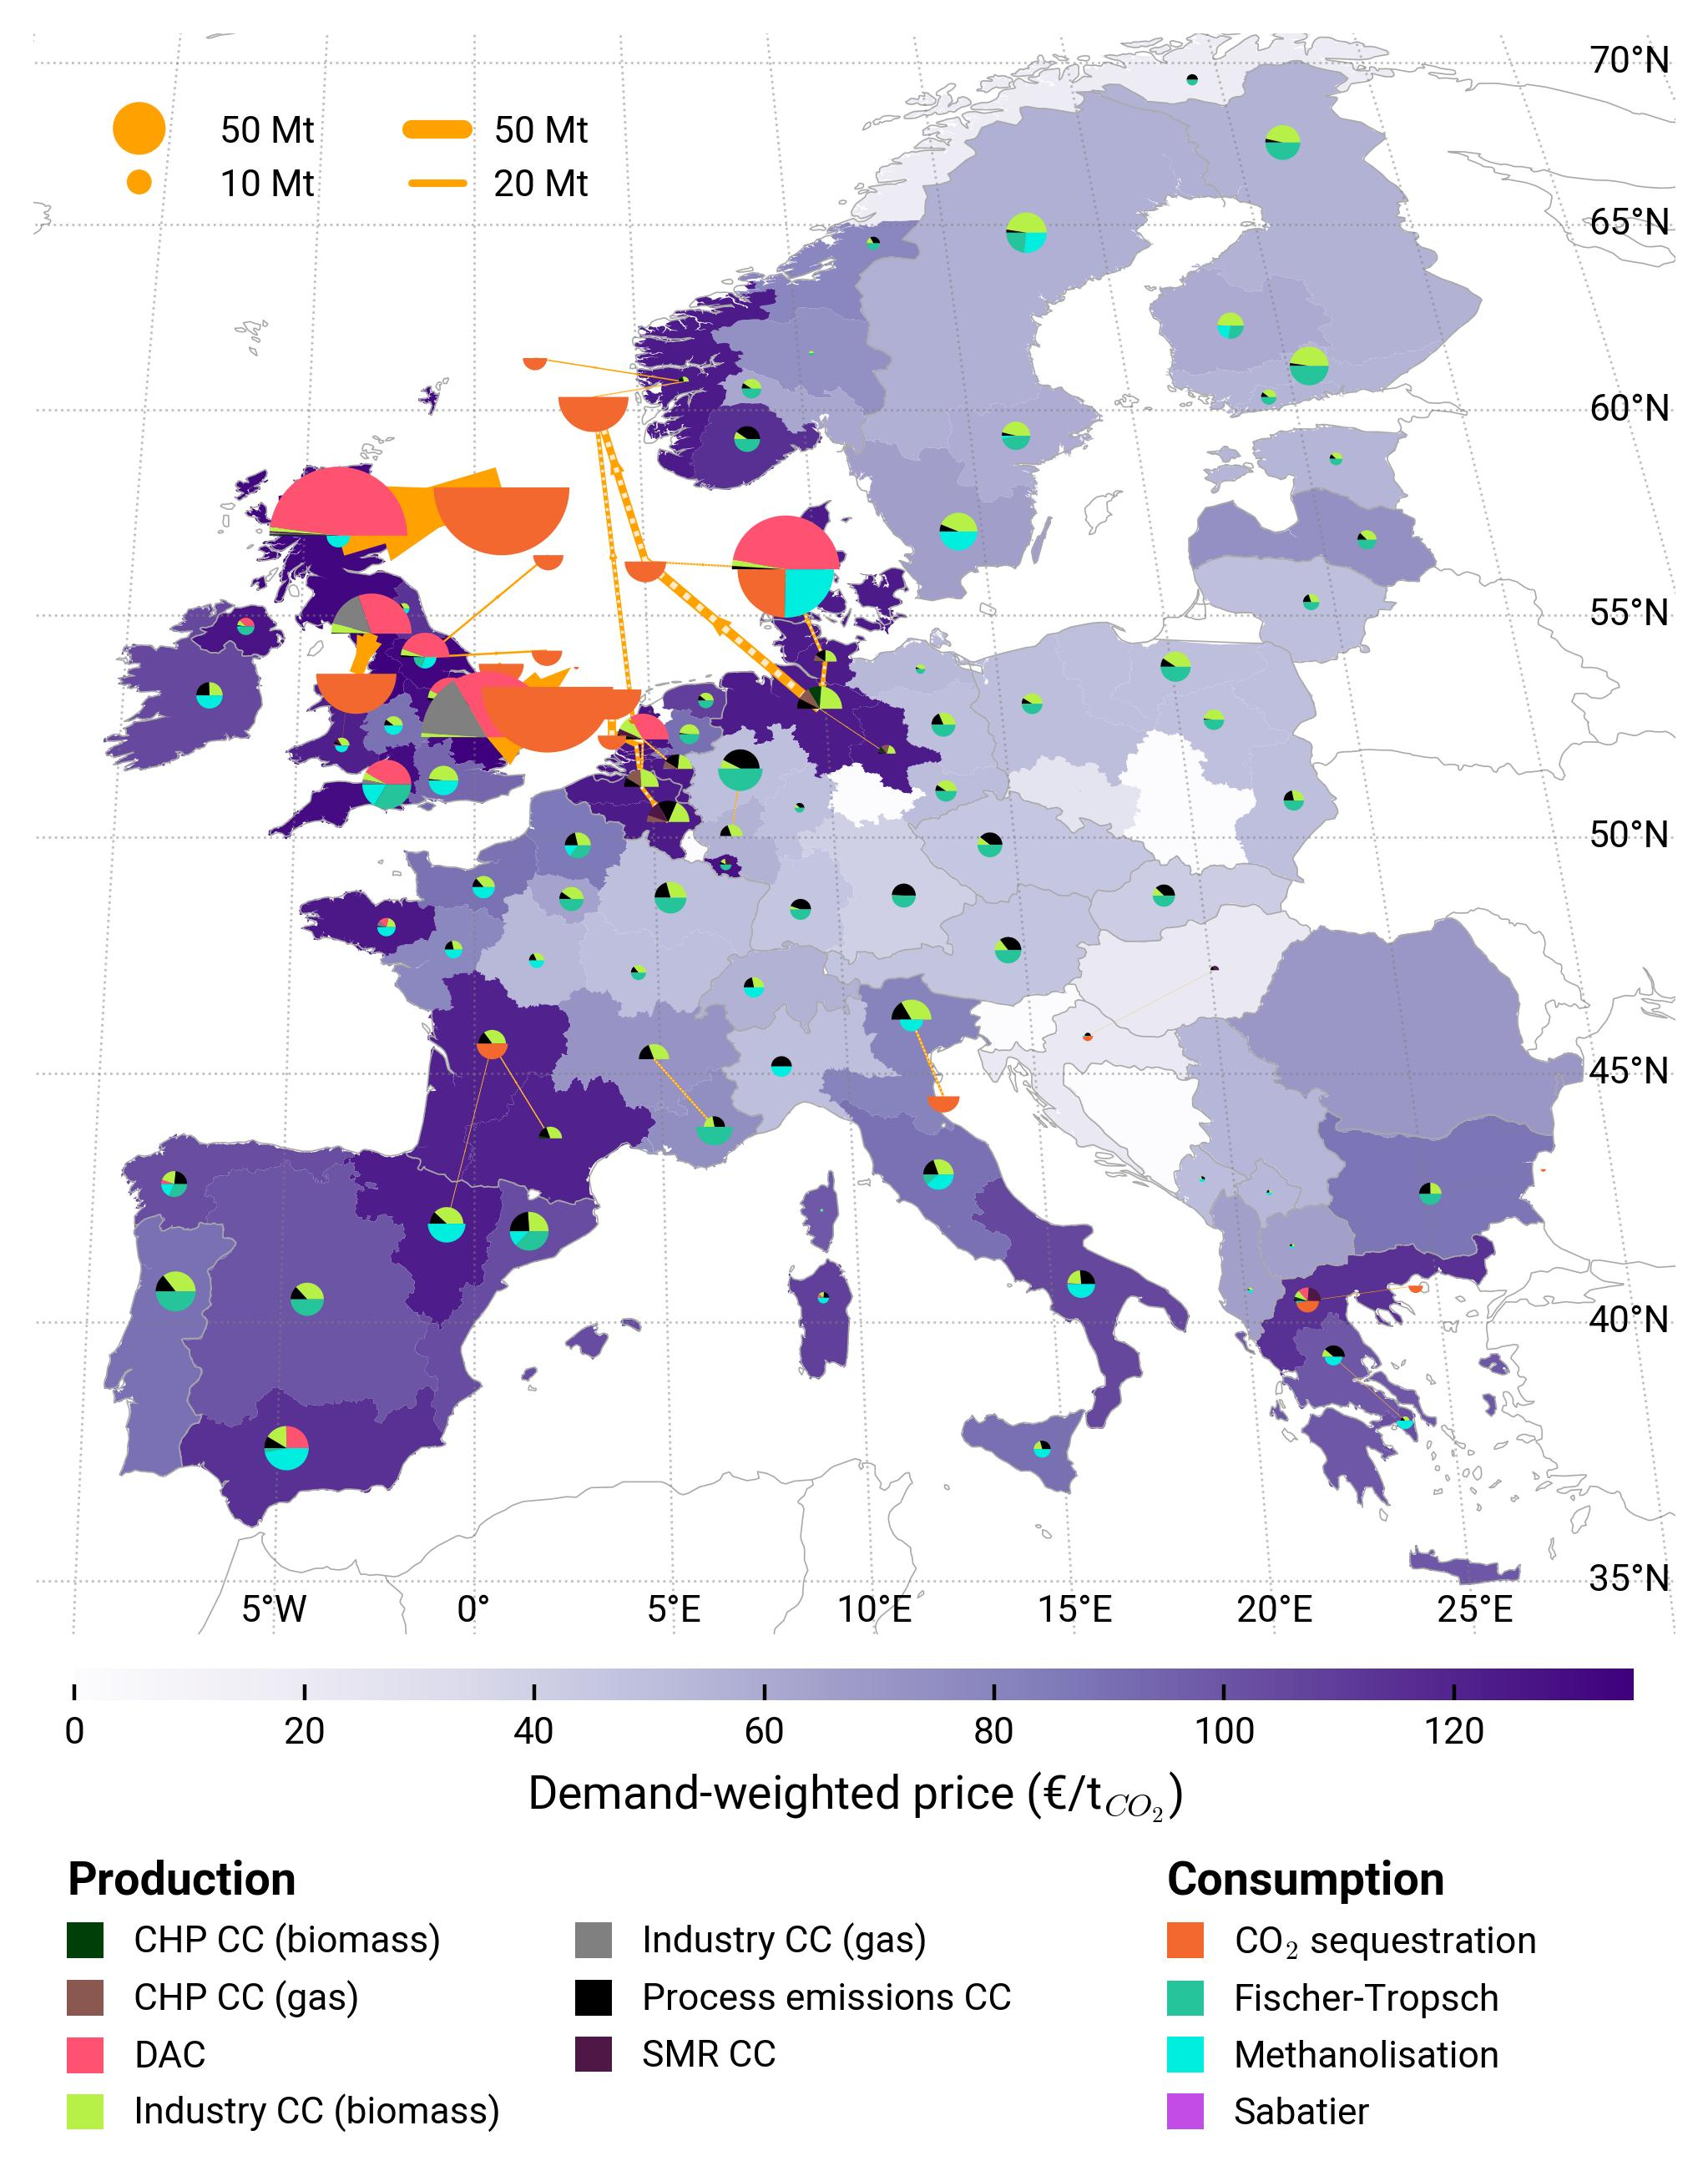
\includegraphics[width=1\textwidth,trim=0cm 0cm 0cm 0cm, clip]{maps/pcipmi/base_s_adm___2050-balance_map_co2_stored} 
      \vspace{-0.7cm}
      \caption{\ce{CO2} 2050.}
      \label{fig:PCI_lt_2050_co2}
  \end{subfigure}
  \caption{\textit{PCI} long-term scenario --- Regional distribution of \ce{H2} and \ce{CO2} production, utilisation, storage, and transport.}
  \label{fig:PCI_lt_2050}
\end{figure*}
\clearpage

\begin{figure*}[htbp]
  \centering
  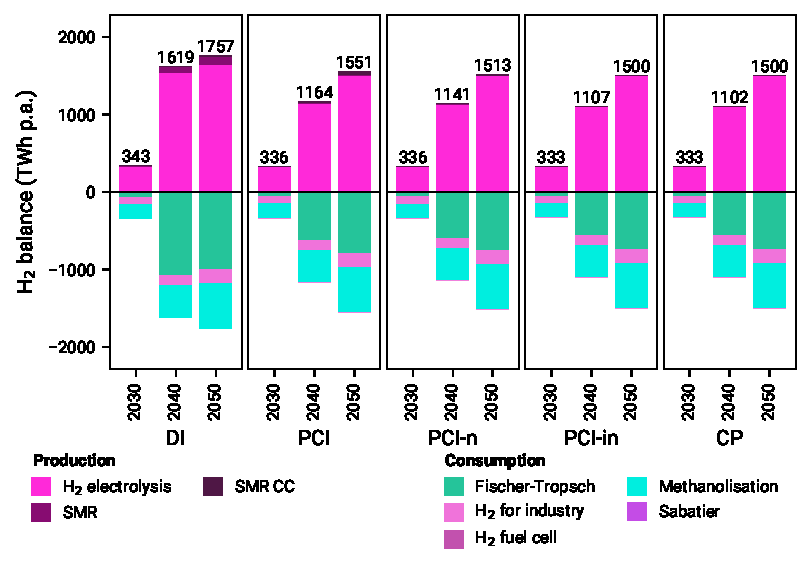
\includegraphics[width=\textwidth]{balances_overview_H2}
  \caption{\ce{H2} balances in long-term scenarios.}
  \label{fig:balances_overview_H2_stored}
\end{figure*}
\paragraph{Hydrogen production and utilisation}
\label{sec:h2_production_and_utilisation}
\ce{H2} production in the model is primarily driven by the demand for Fischer-Tropsch fuels and methanol. In 2030 and 2050, the electrolytic \ce{H2} production target of 10 and 45 Mt p.a. is binding, equivalent to 333 and 1500 TWh p.a. (at a lower heating value of \SI{33.33}{kWh/kg} for \ce{H2}). Only in 2040, the \ce{H2} production target of 27.5 Mt p.a. (917 TWh p.a.) is overachieved by 185-247 TWh p.a. in the \textit{PCI} to \textit{CP} scenarios. \ce{H2} production in the \textit{DI} is significantly higher, given its need for additional Fischer-Tropsch synthesis to bind \ce{CO2} as an alternative to sequestration, as described in the previous section.
In 2050, Fischer-Tropsch fuels are primarily used to satisfy the demand for kerosene in aviation and naphta for industrial processes (see Table \ref{fig:exogenous_demand}). Only about about 93 to 173 TWh p.a. of \ce{H2} is directly used in the industry. Throughout all long-term scenarios, \ce{H2} is almost exclusively produced via electrolysis. Only without any \ce{H2} pipeline infrastructure in the \textit{DI}, the model reverts to steam methane reforming (SMR) to produce 71 to 102 TWh p.a. of \ce{H2} in 2040 and 2050, respectively.
Regionally, \ce{H2} production is concentrated in regions with high solar PV potential such as the Iberian and Italian Peninsula, as well as high wind infeed regions including Denmark, the Netherlands and Belgium. The produced \ce{H2} is then transported via \ce{H2} pipelines including PCI-PMI projects to carbon point sources  in central, continental Europe where it is used as a precursor for Fischer-Tropsch fuels. Onsite \ce{H2} production and consumption primarily occurs in conjunction with methanolisation processes. Figures \ref{fig:PCI_lt_2030_h2}, \ref{fig:PCI_lt_2040_h2}, and \ref{fig:PCI_lt_2050_h2} provide a map of the regional distribution of \ce{H2} production, utilisation, and transport in the \textit{PCI} scenario. Additional maps are provided in \ref{sec:maps}. Note that PCI-PMI projects or candidates (in \textit{CP} scenario) are plotted in dotted white lines.

\todo[inline]{TODO: Add section on H2 pipeline utilisation
maybe histogram with all years overlapping in different colours}

\subsection{Performance in short-term scenarios}
\label{sec:short-term_scenarios_performance}

In this section, we assess the impact of the short-term scenarios on the long-term scenarios, by comparing the economic regret, as well as the impact on \ce{CO2} utilisation and sequestration, \ce{H2} production. 

\paragraph{Regret analysis}
\label{sec:regret_analysis}
We calculate the regret terms by subtracting the annual total system costs of the long-term scenarios (row) from the short-term scenarios (columns). Positive values reflect higher costs in the short-term scenarios compared to the long-term ones. Figure \ref{fig:regret_matrix_results} shows the regret matrix for all scenarios and planning horizons. From left to right, the first column shows the regret terms for the \textit{Reduced targets} scenario, where all long-term targets are removed except for the GHG emission reduction target. The second column shows the regret terms for the \textit{Delayed pipelines} scenario, where all PCI-PMI and endogenous pipelines are delayed by one period. The third column shows the regret terms for the \textit{No pipelines} scenario, where all pipeline capacities are removed.

In the \textit{Reduced targets} scenario, system costs barely change through the relaxation of the targets. The long-term results have shown that the model was overachieving the \ce{H2} production targets in 2040. As for the \ce{CO2} sequestration targets, the model is still incentivised by GHG emission targets, especially in 2040 and 2050. Only in 2030, we see minimal changes in total system costs, as the 2030 targets are not cost-optimal. However, they are required to stimulate the build-out necessary to reach 2040 and 2050 targets. In all of the long-term scenarios, we have observed that in 2030 that especially \ce{CO2} pipeline infrastructure is not essential yet (see Figure \ref{fig:CP_lt_2030_co2}). As for \ce{H2} pipeline infrastructure, the solution space seems to be quite flat, as the costs for the \textit{DI} scenario without any pipelines (Figure \ref{fig:DI_lt_2030_co2}) and the \textit{CP} scenario (Figure \ref{fig:CP_lt_2030_co2}) with notable pipeline investments are almost identical. By removing the \ce{H2} production and \ce{CO2} sequestration targets, pipelines become even less relevant, although the cost savings due to the dropped targets are minimal, ranging from 4.3 to 5 bn. \euro{} p.a. in 2030 and 2040.

\begin{figure*}[htbp]
  \centering
  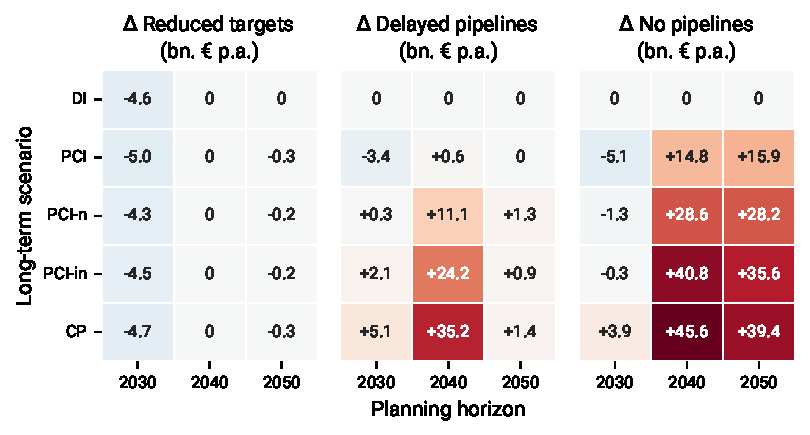
\includegraphics[width=\textwidth]{regret_matrix}
  \caption{Regret matrix. Calculating regret terms by subtracting system costs of long-term scenarios (rows) from short-term scenarios (columns). Positive values reflect higher costs in the short-term scenarios compared to the long-term ones.}
  \label{fig:regret_matrix_results}
\end{figure*}

For the same reasons, the 2030 results for the \textit{Delayed pipelines} and \textit{No pipelines} scenarios show only minor differences in system costs compared to the long-term scenarios. Cost savings of 3.4 to 5.1 bn. \euro{} p.a. in the \textit{PCI} long-term scenario indicate that for 2030, forcing in PCI-PMI projects is not cost- and topologically optimal in the short run. Whereas slight regret/cost increase of 3.9 to 5.1 bn \euro{} p.a. in the \textit{CP} shows a small dependency on the invested pipeline infrastructure (Figure \ref{fig:CP_lt_2030}), being the most cost-optimal solution.

When looking at the more long-term perspective, we see significant regrets in the \textit{Delayed pipelines} and \textit{No pipelines} scenarios. Having originally planned the energy system layout (incl. generation, transport, conversion technologies and storage) in the long-term scenario with PCI-PMI projects and/or endogenous pipelines, the model has to find alternative investments to still meet all targets, as the pipelines now materialise one period later or not at all. Regrets peak in 2040, where a delay of pipelines costs the system between 0.6 to 24.2 bn. \euro{} p.a. in the scenarios with PCI-PMI projects and up to 35.2 bn. \euro{} p.a. in the \textit{CP} scenario. 2050 regrets are lower than 2040 regrets, as almost all PCI-PMI pipelines are originally commissioned by 2030. So a delay of projects from 2040 to 2050 only mildly impacts the system costs by 0.6 bn. \euro{} p.a. The more pipelines invested beyond those of PCI-PMI projects, the higher the regret if they are delayed. In 2050, very few additional \ce{CO2} and \ce{H2} pipelines are built, as such, a delay only increases system costs by 0.9 to 1.4 bn. \euro{} p.a. 
The short-term scenario \textit{No pipelines} shows the highest regrets, ranging from 14.8 to 45.6 bn. \euro{} p.a. in 2040 and 15.9 to 39.4 bn. \euro{} p.a. in 2050. Note that this scenario serves more of a hypothetical worst case as it is not likely to build out an energy system with pipelines in mind but none materialising at all.

Consistently throughout all short-term scenarios, most of the additional cost stem from the need to invest into additional carbon capture, renewable generation, and conversion technologies (see Figure \ref{fig:capacities_overview_extended}). Additional renewable generation capacities are made up of solar PV and wind. A significant higher amount of electrolyser capacity of more than 50 GW is needed in 2040 if pipelines are delayed. 

\paragraph{Carbon capture}
Further, the model has to invest in more than 28 GW of carbon capture units at point sources and an additional 14 GW in DAC technologies to meet the sequestration and emission reduction targets. Cost-wise, the short-term investments into DAC technologies make up to a half of the of the additional system costs in both the \textit{Delayed pipelines} and \textit{No pipelines} scenarios (see Figure \ref{fig:costs_overview_extended}). DAC utilisation can increase from 40 Mt p.a. in the \textit{PCI-n} to more than 200 Mt p.a. in the \textit{CP} scenario when pipelines are delayed (see Figure \ref{fig:balances_overview_extended_co2_stored}). If pipelines are not built at all, additional 60 Mt p.a. in the \textit{PCI} up to 250 Mt p.a. in the \textit{CP} scenario are captured from DAC, substituting a large share of \ce{CO2} previously captured from point sources equipped with carbon capture (biomass-based industry processes and non-abatable process emissions).

Note that a clear trade-off between the reliance on pipeline infrastructure and the need for DAC technologies can be observed in Figure \ref{fig:delta_balances_dac}. While the reliance on DAC decreases with the build-out of pipeline infrastructure, the model in return has to invest in more DAC if pipelines are delayed or not built at all. There is a risk involved, that the need for DAC is even higher in the scenarios with pipeline infrastructure compared to the \textit{DI} scenario, especially in later years (2040 and 2050), if the pipelines do not materialise at all, seeing a potential increase of 50 Mt p.a. in 2040 and 80 Mt p.a. in 2050 in the \textit{PCI} scenario.

\begin{figure}[htbp]
  \centering
  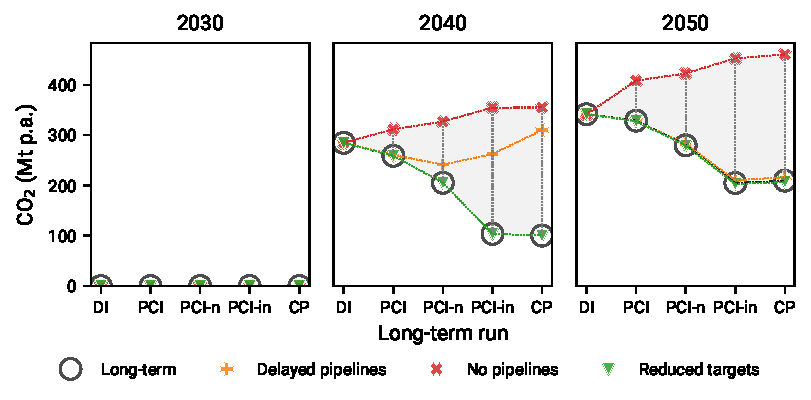
\includegraphics[width=\textwidth]{delta_balances_DAC}
  \caption{Delta balances --- \ce{CO2} from Direct Air Capture.}
  \label{fig:delta_balances_dac}
\end{figure}


\paragraph{\ce{H2} production} 
On the \ce{H2} side, we find that the electrolytic \ce{H2} production target of 10 Mt p.a. (333 TWh p.a.) in 2030 is overly ambitious. Figure \ref{fig:balances_overview_extended_H2_stored} shows that in the \textit{Reduced targets} scenario, 132 to 151 TWh p.a. of \ce{H2}, corresponding to almost half of the target is produced from SMR instead of electrolysis. When pipelines are delayed, the model has to fall back to more decentral \ce{H2} production of an additional 55 to 187 TWh p.a. of \ce{H2} from electrolysis, SMR and SMR with carbon capture (the latter being the most expensive option). In the \textit{No pipelines} scenario, this additional \ce{H2} production increases to up to 305 TWh p.a (see Figure \ref{fig:balances_overview_extended_H2_stored}).

\subsection{Value of PCI-PMI projects}
\label{sec:value_of_pcipmi_projects}
Looking at long-run we find that PCI-PMI projects, while not completely cost-optimal compared to a centrally planned system, are still cost-beneficial. Compared to a complete lack of \ce{H2} and \ce{CO2} pipeline infrastructure as well as lower \ce{CO2} sequestration potential, the \textit{PCI} scenario unlocks annual cost savings in up to 30.7 bn. \euro{} p.a. Figure \ref{fig:totex_heatmap} shows the total system costs (TOTEX) p.a. split into CAPEX and OPEX p.a., as well as the net present value of total system costs (NPV) until 2060, discounted at an interest rate of \SI{7}{\percent} p.a.
Even when accounting for the additional costs of 0.6 bn. \euro{} faced in the \textit{Delayed pipelines} and up to 15.9 bn. \euro{} p.a. in the \textit{No pipelines} scenario, a net positive is achieved, indicating that investing into the PCI-PMI infrastructure is a no-regret option. By connecting further \ce{H2} production sites and \ce{CO2} point sources to the pipeline network. additional cost savings of up to 18.4 bn. \euro{} p.a. can be achieved in the \textit{PCI-in} scenario. The \textit{CP} scenario serves as a theoretical benchmark, allowing the model to invest freely, not bound by \textit{forced} PCI-PMI projects. The model can invest in fewer, but more optimally located \ce{CO2} and \ce{H2} pipelines from a systemic perspective. Economic benefits of all pipeline investments materialise after 2030, yielding lower net present values (NPV) of total system costs of potentially at least 75 bn. \euro{} over the course of the assets' lifetime. 

\begin{figure*}[htbp]
  \centering
  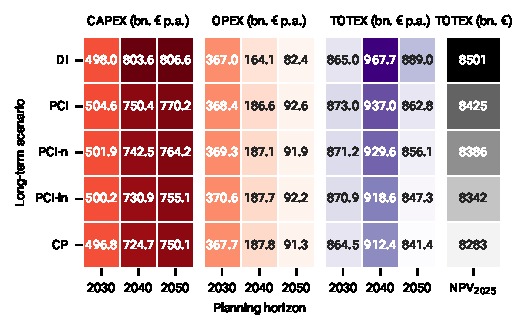
\includegraphics[width=\textwidth]{totex_heatmap.pdf}
  \caption{Annual system costs by long-term scenario and planning horizon.}
  \label{fig:totex_heatmap}
\end{figure*}

\clearpage

\subsection{Limitations of our study}
\label{sec:limitations}
While our study assesses a variety of topologies, planning horizons, and potential regret scenarios, it is not exhaustive and comes with limitations.
As we focus on the impact of continental European PCI-PMI infrastructure, we neglect fuel and energy imports from outside Europe. \ce{H2} and \ce{CO2} demand is directly driven by fixed, exogenous demands for the respective carrier or their derivatives.

Regarding the modelling of both \ce{H2} and \ce{CO2} pipelines, we assume a level playing field for all pipeline projects through standardised costs and applying haversine distance, i.e., no discrimination between PCI-PMI projects and other projects, this is a simplification as real costs may differ. We also do not discretise the endogenously built pipelines (due to computational complexity) and allow any capacity to be built. This assumption can lead to underestimation of the true costs of pipeline investments.

Further, all results are based on a single weather year, i.e., 2013.
Other limitations include geographic and temporal clustering to make the problem solving computationally feasible.
\section{Conclusion}
\label{sec:conclusion}

In this study, we have assessed the impact of PCI-PMI projects on reaching European climate targets on its path to net-zero by 2050. We have modelled the European energy system with a focus on \ce{H2} and \ce{CO2} infrastructure, and evaluated the performance of different levels of pipeline roll-out under three short-term scenarios. 


\paragraph{Economic viability and policy targets}
Our findings demonstrate that PCI-PMI \ce{CO2} and \ce{H2} infrastructure generate a net positive impact on total system costs, even when accounting for potential additional costs involved with the delay of pipelines. This positions PCI-PMI projects as a no-regret investment option for the European energy system. 
Their economic benefit increases considerably when strategic pipeline extensions are implemented, connecting additional \ce{H2} production sites and \ce{CO2} point sources to the pipeline network. 
Compared to a system without any pipeline infrastructure, PCI-PMI projects help to achieve the EU's ambitious policy targets, including net-zero emissions, \ce{H2} production and \ce{CO2} sequestration targets, while reducing system costs and technology dependencies.

\paragraph{CCUS and hydrogen utilisation}
The pipeline infrastructure serves dual purposes in Europe's decarbonisation strategy, \ce{H2} pipelines facilitate the distribution of more affordable green \ce{H2} from northern and south-western regions rich in renewable energy potential to high-demand regions in central Europe. Complementarily, \ce{CO2} transport and offshore sequestration sites enable industrial decarbonisation by linking major industrial sites and their process emissions to offshore sequestration sites in the North Sea, particularly in Denmark, Norway, and the Netherlands.

\paragraph{Technology diversification}
The build-out of pipelines serves as an essential risk hedging mechanism against overbuilding solar and wind generation capacities while reducing excessive reliance on singular carbon capture technologies such as direct air capture (DAC) and point-source carbon capture, confirming the findings of \cite{hofmannH2CO2Network2025}. This diversification further enhances system resilience towards uncertainties involved with technologies that are not yet commercially available at scale, such as DAC.

\paragraph{Political support and public acceptance} 
While PCI-PMI may not achieve perfect cost-optimality in their entirety compared to a theoretically centrally planned system, they possess benefits beyond pure economic viability. The success of large-scale infrastructure investments highly depend on continuous political support and public acceptance --- factors that are particularly favourable for PCI-PMI projects. Being directly supported by the European Commission, PCI-PMI projects see stronger political backing, institutional support structures with regard to financing, access to grants, acceleration in permitting processes. Being required to frequent and transparent progress reports, PCI-PMI projects are more likely to be accepted by the public.


\clearpage
\section*{CRediT authorship contribution statement}
\textbf{Bobby Xiong}: Conceptualisation, Methodology, Software, Validation, Investigation, Data Curation, Writing --- Original Draft, Review \& Editing, Visualisation. \textbf{Iegor Riepin}: Conceptualisation, Methodology, Investigation, Writing --- Review \& Editing, Project Administration, Funding acquisition. \textbf{Tom Brown}: Investigation, Resources, Writing --- Review \& Editing, Supervision, Funding acquisition.

\section*{Declaration of competing interest}
The authors declare that they have no known competing financial interests or personal relationships that could have appeared to influence the work reported in this paper.

\section*{Data and code availability}
All results, including solved PyPSA networks and summaries in .csv format are published on Zenodo: \newline
\href{https://doi.org/XX.YYYY/zenodo.10000000}{https://doi.org/XX.YYYY/zenodo.10000000}

The entire workflow, including the custom model based on PyPSA-Eur v2025.01.0, PCI-PMI project implementation, regret-matrix setup, postprocessing and visualisation routines can be completely reproduced from the GitHub repository: \newline 
\href{https://github.com/bobbyxng/pcipmi-policy-targets}{https://github.com/bobbyxng/pcipmi-policy-targets}

\section*{Acknowledgements}
This work was supported by the German Federal Ministry for Economic Affairs and Climate Action (BMWK) under Grant No. 03EI4083A (RESILIENT). This project has been funded by partners of the CETPartnership (\href{https://cetpartnership.eu}{https://cetpartnership.eu}) through the Joint Call 2022. As such, this project has received funding from the European Union's Horizon Europe research and innovation programme under grant agreement no. 101069750.


%% The Appendices part is started with the command \appendix;
%% appendix sections are then done as normal sections
\newpage
\appendix

\section{Supplementary material --- Data}
\label{app:data}\begin{figure*}[htbp]
  \centering
  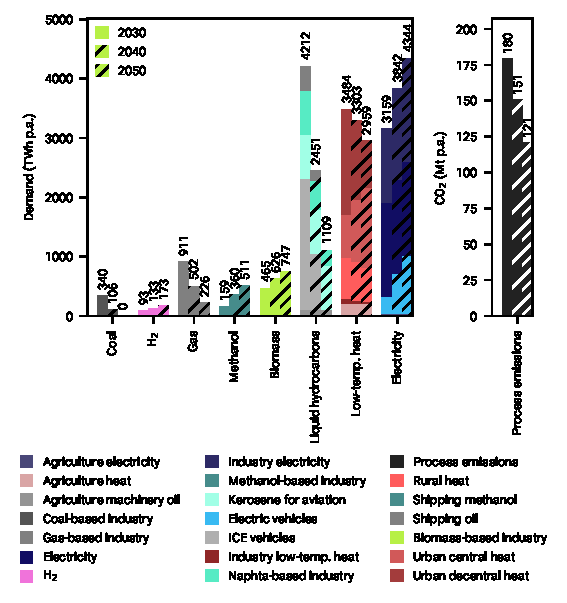
\includegraphics[width=\textwidth]{exogenous_demand.pdf}
  \caption{Exogenous demand.}
  \label{fig:exogenous_demand}
\end{figure*}

\clearpage
\section{Supplementary material --- Methodology}
\label{app:methodology}

\begin{table*}[htbp]
  \centering
  \caption{Regional clustering: A total of 99 regions are modelled, excl. offshore buses.}
  \label{tab:regional_clustering}
  \scriptsize
  \begin{tabularx}{\textwidth}{R{3.9cm}>{\centering\arraybackslash}X>{\centering\arraybackslash}X}
    \toprule
     & \textbf{Country} & \textbf{Buses} \\
    \midrule
    \textbf{Administrative level} & $\bm\sum$ & \textbf{99} \\
    NUTS2 & Finland (FI) & 4 \\
          & Norway (NO) & 6 \\
    \midrule
    NUTS1 & Belgium (BE)** & 2 \\
          & Switzerland (CH) & 1 \\
          & Czech Republic (CZ) & 1 \\
          & Germany (DE)* & 13 \\
          & Denmark (DK) & 1 \\
          & Estonia (EE) & 1 \\
          & Spain (ES)* & 5 \\
          & France (FR) & 13 \\
          & Great Britain (GB)* & 11 \\
          & Greece (GR) & 3 \\
          & Ireland (IE) & 1 \\
          & Italy (IT)* & 6 \\
          & Lithuania (LT) & 1 \\
          & Luxembourg (LU) & 1 \\
          & Latvia (LV) & 1 \\
          & Montenegro (ME) & 1 \\
          & Macedonia (MK) & 1 \\
          & Netherlands (NL) & 4 \\
          & Poland (PL) & 7 \\
          & Portugal (PT) & 1 \\
          & Sweden (SE) & 3 \\
          & Slovenia (SI) & 1 \\
          & Slovakia (SK) & 1 \\
    \midrule
    NUTS0 & Albania (AL) & 1 \\
          & Austria (AT) & 1 \\
          & Bosnia and Herzegovina (BA) & 1 \\
          & Bulgaria (BG) & 1 \\
          & Croatia (HR) & 1 \\
          & Hungary (HU) & 1 \\
          & Romania (RO) & 1 \\
          & Serbia (RS) & 1 \\
          & Kosovo (XK) & 1 \\
    \bottomrule
  \end{tabularx}
  \caption*{\scriptsize City-states (*) (i.e., Berlin, Bremen, Hamburg, Madrid, and London) and regions without substations (**) (one in BE) are merged with neighbours. Sardinia and Sicily are modelled as two separate regions.}
\end{table*}

\begin{table*}
  \centering
  \caption{DUMMY Overview of technology cost assumptions. TODO compare with FLEITER PAPER TABLE 9}
  \label{tab:cost_assumptions}
  \scriptsize
  \begin{tabularx}{\textwidth}{R{3.9cm}>{\centering\arraybackslash}X>{\centering\arraybackslash}X>{\centering\arraybackslash}X>{\centering\arraybackslash}X}
    \toprule
    & \textbf{Unit} & \textbf{2030} & \textbf{2040} & \textbf{2050} \\
    \midrule
    \textbf{Technology} & & & & \\
    CO2 pipelines & XX & 1000 & 1000 & 1000 \\
    Onshore, offshore & XX & 1000 & 1000 & 1000 \\
    Electrolysers & XX & 1000 & 1000 & 1000 \\
    \bottomrule
  \end{tabularx}
\end{table*}

\clearpage
\section{Supplementary material --- Results and discussion}
\label{app:results_and_discussion}
\subsection{Installed capacities}
\label{sec:installed_capacities}
\begin{figure*}[htbp]
  \centering
  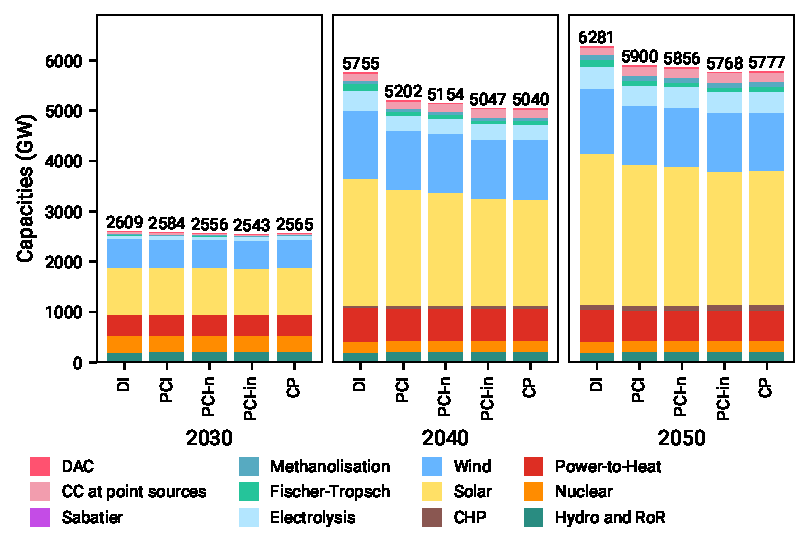
\includegraphics[width=\textwidth]{capacities_overview.pdf}
  \caption{Installed capacities in long-term scenarios.}
  \label{fig:capacities_overview}
\end{figure*}

\clearpage
\subsection{Delta capacities}
\label{sec:delta_system_costs}
\begin{figure*}[htbp]
  \centering
  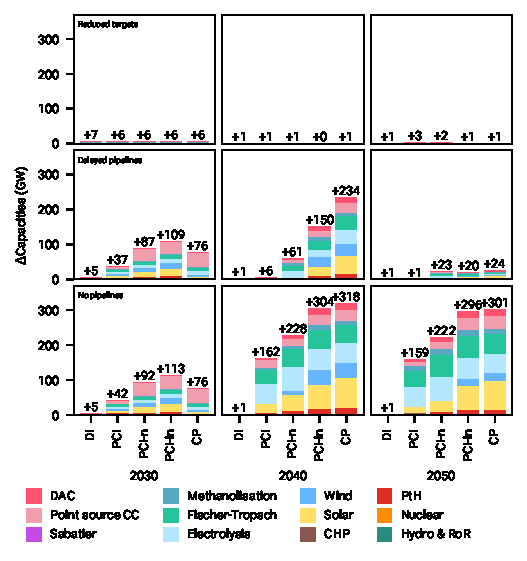
\includegraphics[width=\textwidth]{capacities_overview_extended.pdf}
  \caption{$\Delta$Capacities --- Short-term minus long-term runs.}
  \label{fig:capacities_overview_extended}
\end{figure*}


\clearpage
\subsection{Delta system costs}
\label{sec:delta_system_costs}
\begin{figure*}[htbp]
  \centering
  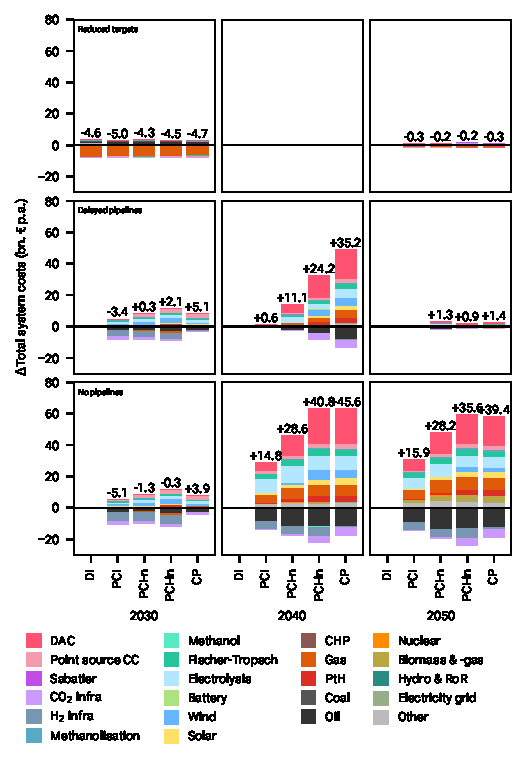
\includegraphics[width=\textwidth]{costs_overview_extended.pdf}
  \caption{$\Delta$System costs --- Short-term minus long-term runs.}
  \label{fig:costs_overview_extended}
\end{figure*}

\clearpage
\subsection{Delta balances}
\begin{figure*}[htbp]
  \centering
  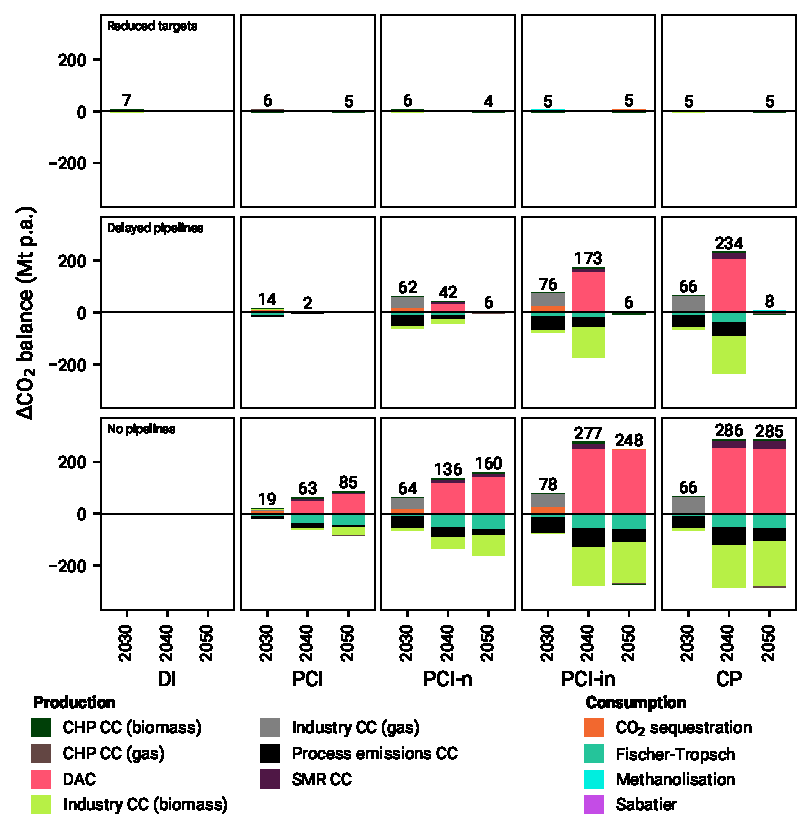
\includegraphics[width=\textwidth]{balances_overview_extended_co2 stored}
  \caption{$\Delta$\ce{CO2} balances --- Short-term minus long-term runs.}
  \label{fig:balances_overview_extended_co2_stored}
\end{figure*}
\begin{figure*}[htbp]
  \centering
  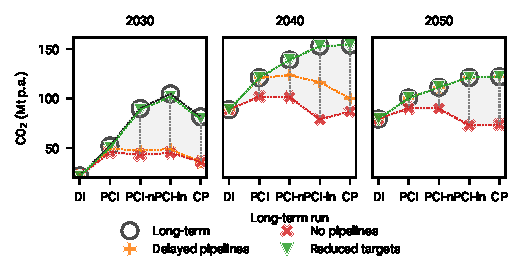
\includegraphics[width=\textwidth]{delta_balances_process emissions CC}
  \caption{$\Delta$\ce{CO2} balances --- Process emissions including Carbon Capture.}
  \label{fig:delta_balances_process_emissions_CC}
\end{figure*}

\begin{figure*}[htbp]
  \centering
  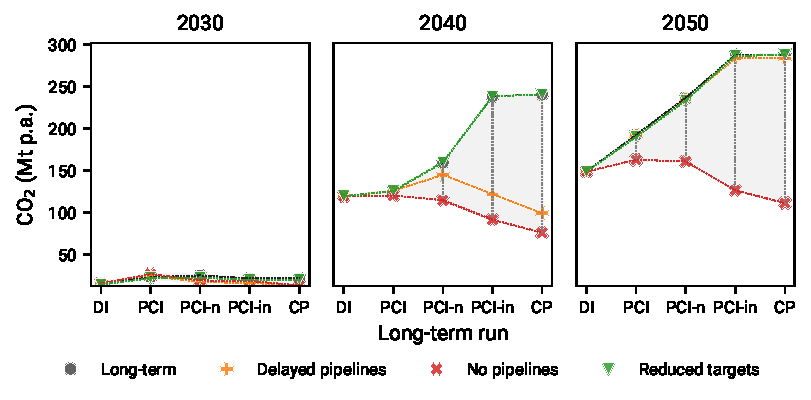
\includegraphics[width=\textwidth]{delta_balances_solid biomass for industry CC}
  \caption{$\Delta$\ce{CO2} balances --- Carbon capture from solid biomass for industry point sources.}
  \label{fig:delta_balances_biomass_industry_cc}
\end{figure*}

\begin{figure*}[htbp]
  \centering
  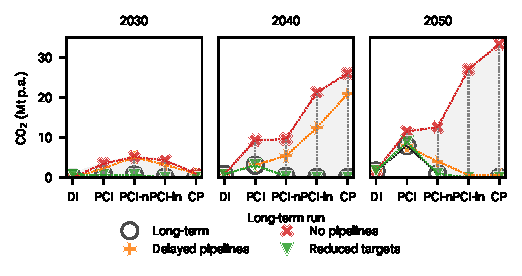
\includegraphics[width=\textwidth]{delta_balances_SMR CC}
  \caption{$\Delta$\ce{CO2} balances --- Carbon capture from steam methane reforming point sources.}
  \label{fig:delta_balances_smr_cc}
\end{figure*}

\begin{figure*}[htbp]
  \centering
  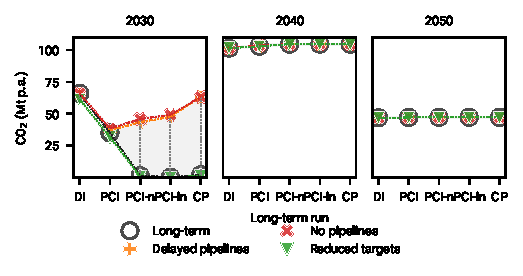
\includegraphics[width=\textwidth]{delta_balances_gas for industry CC}
  \caption{$\Delta$\ce{CO2} balances --- Carbon captured from gas for industry point sources.}
  \label{fig:delta_balances_gas_for_industry}
\end{figure*}

\begin{figure*}[htbp]
  \centering
  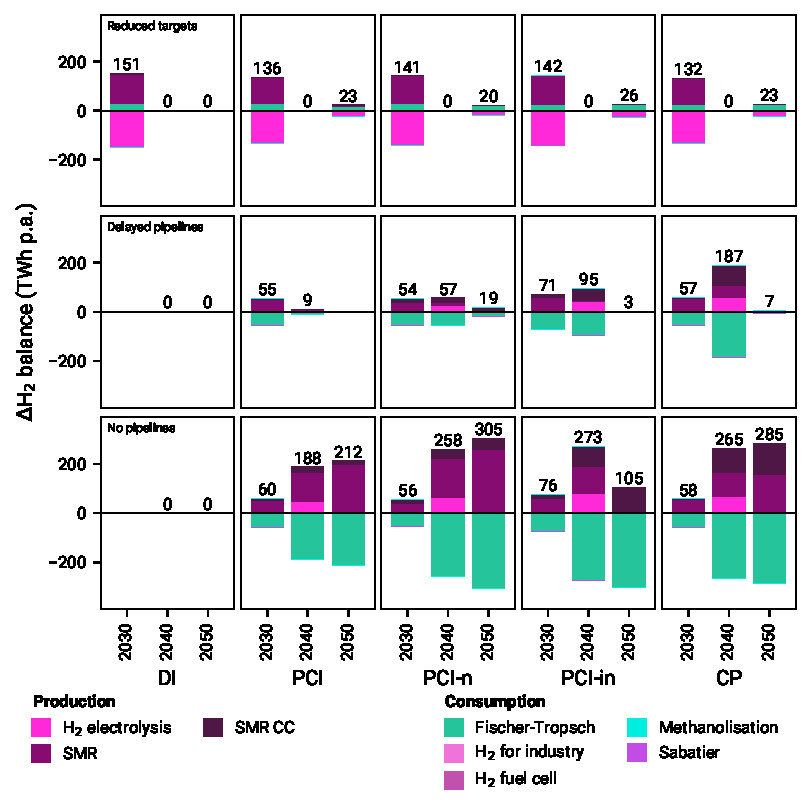
\includegraphics[width=\textwidth]{balances_overview_extended_H2}
  \caption{$\Delta$\ce{H2} balances --- Short-term minus long-term runs.}
  \label{fig:balances_overview_extended_H2_stored}
\end{figure*}

\begin{figure*}[htbp]
  \centering
  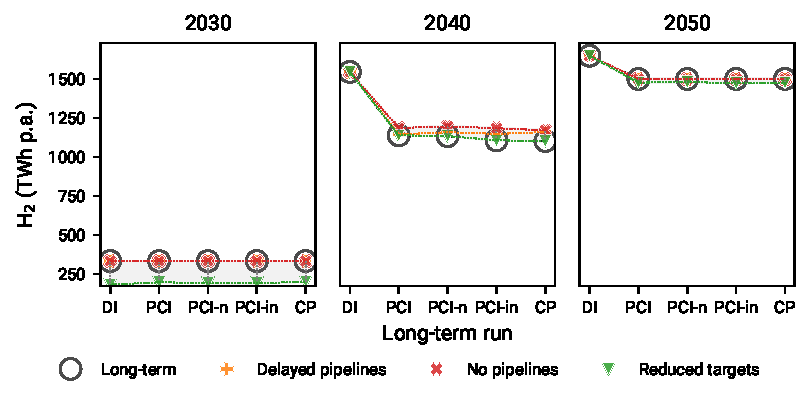
\includegraphics[width=\textwidth]{delta_balances_H2 Electrolysis}
  \caption{Delta balances --- Electrolytic \ce{H2} production}
  \label{fig:delta_balances_h2_electrolysis}
\end{figure*}

\begin{figure*}[htbp]
  \centering
  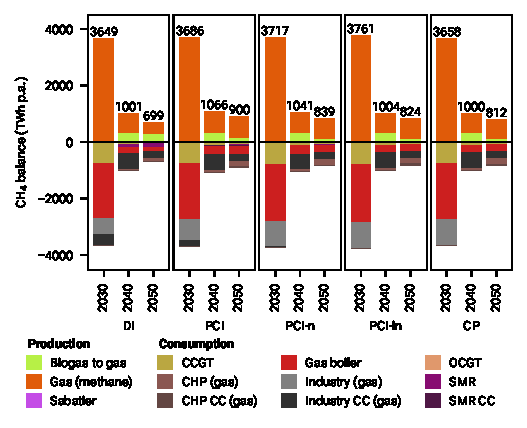
\includegraphics[width=\textwidth]{balances_overview_gas}
  \caption{\ce{CH4} balances in long-term scenarios.}
  \label{fig:balances_overview_gas}
\end{figure*}

\begin{figure*}[htbp]
  \centering
  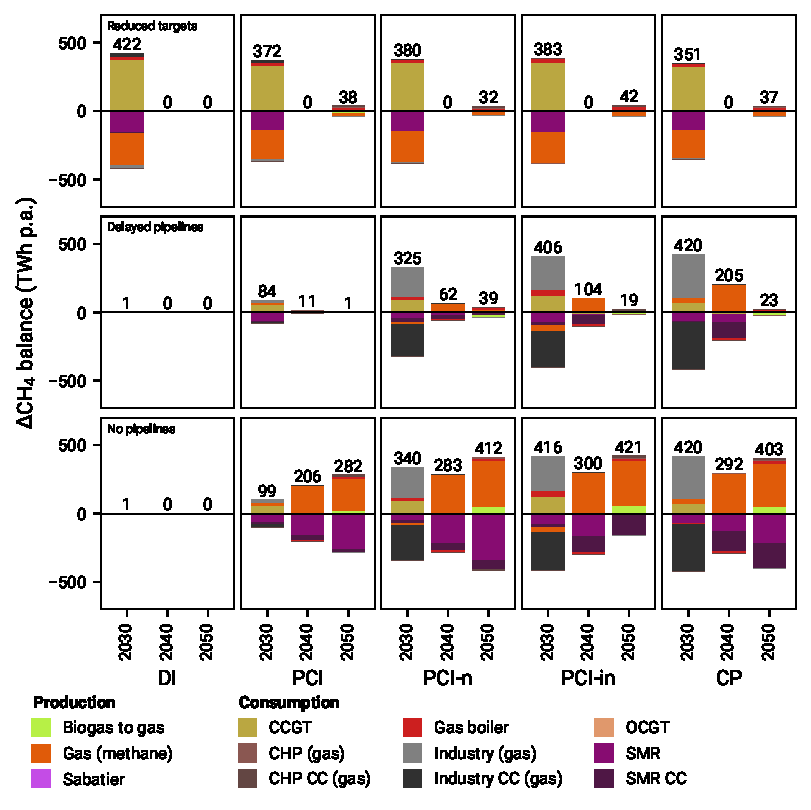
\includegraphics[width=\textwidth]{balances_overview_extended_gas}
  \caption{$\Delta$\ce{CH4} balances --- Short-term minus long-term runs.}
  \label{fig:balances_overview_extended_gas}
\end{figure*}


\clearpage
\subsection{Maps}
\label{sec:maps}
\subsubsection{Decentral Islands}
\begin{figure*}[htbp]
  \centering
  \begin{subfigure}[t]{0.49\textwidth}
      \vspace{0pt}
      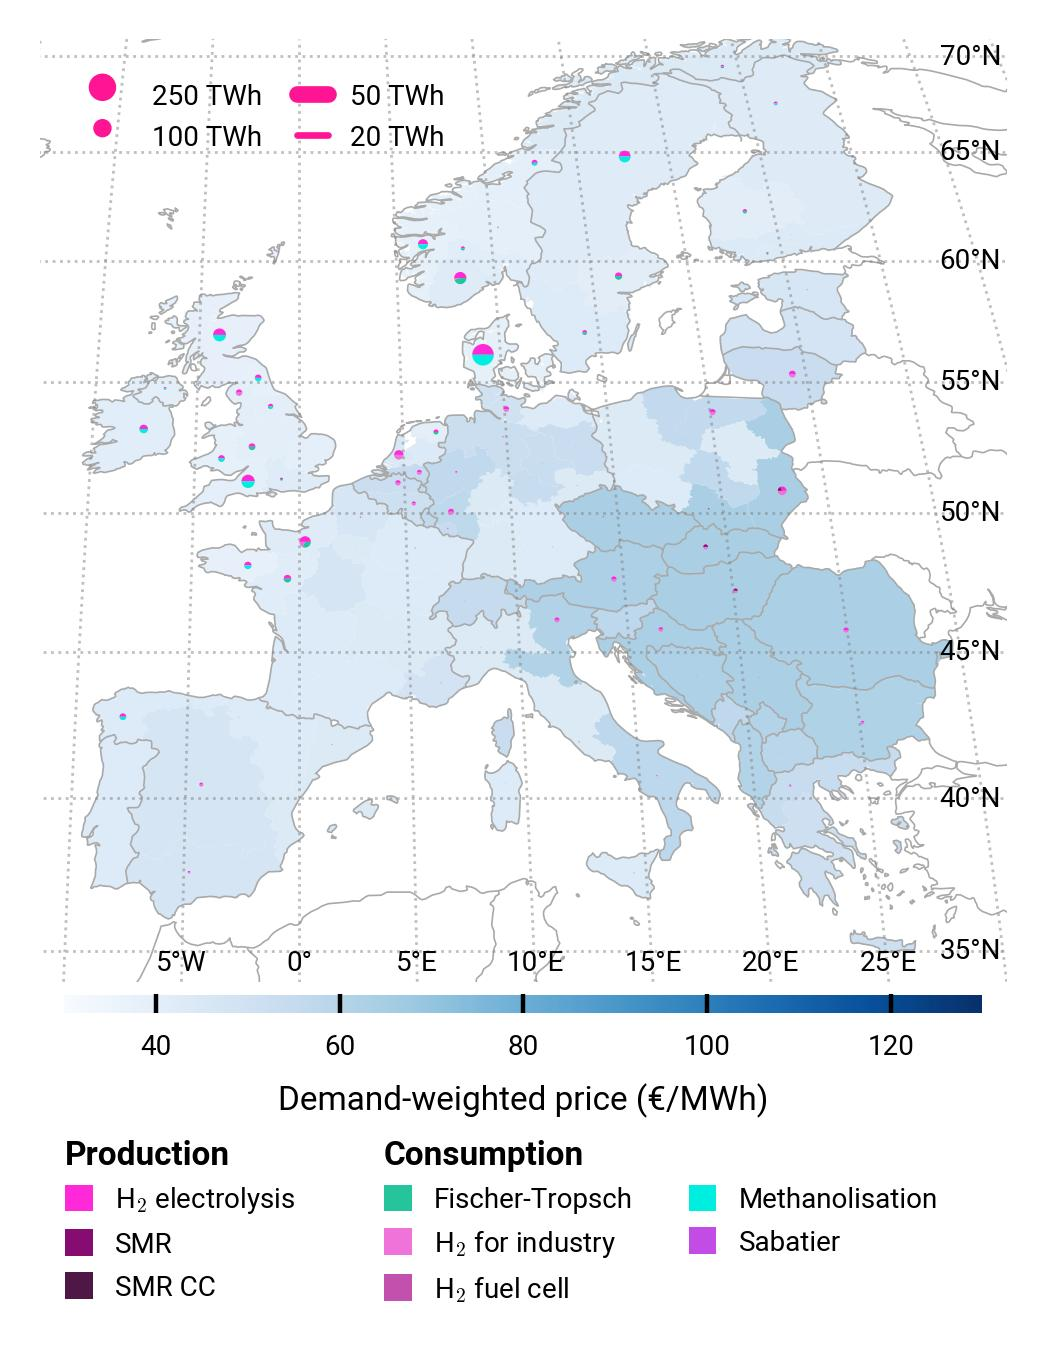
\includegraphics[width=1\textwidth]{maps/no-pipelines-no-pcipmi/base_s_adm___2030-balance_map_H2}
      \vspace{-0.5cm}
      \caption{\ce{H2} regional balances and flows.}
      \label{fig:DI_lt_2030_h2}
  \end{subfigure}
  \hfill
  \begin{subfigure}[t]{0.49\textwidth}
      \vspace{0pt}
      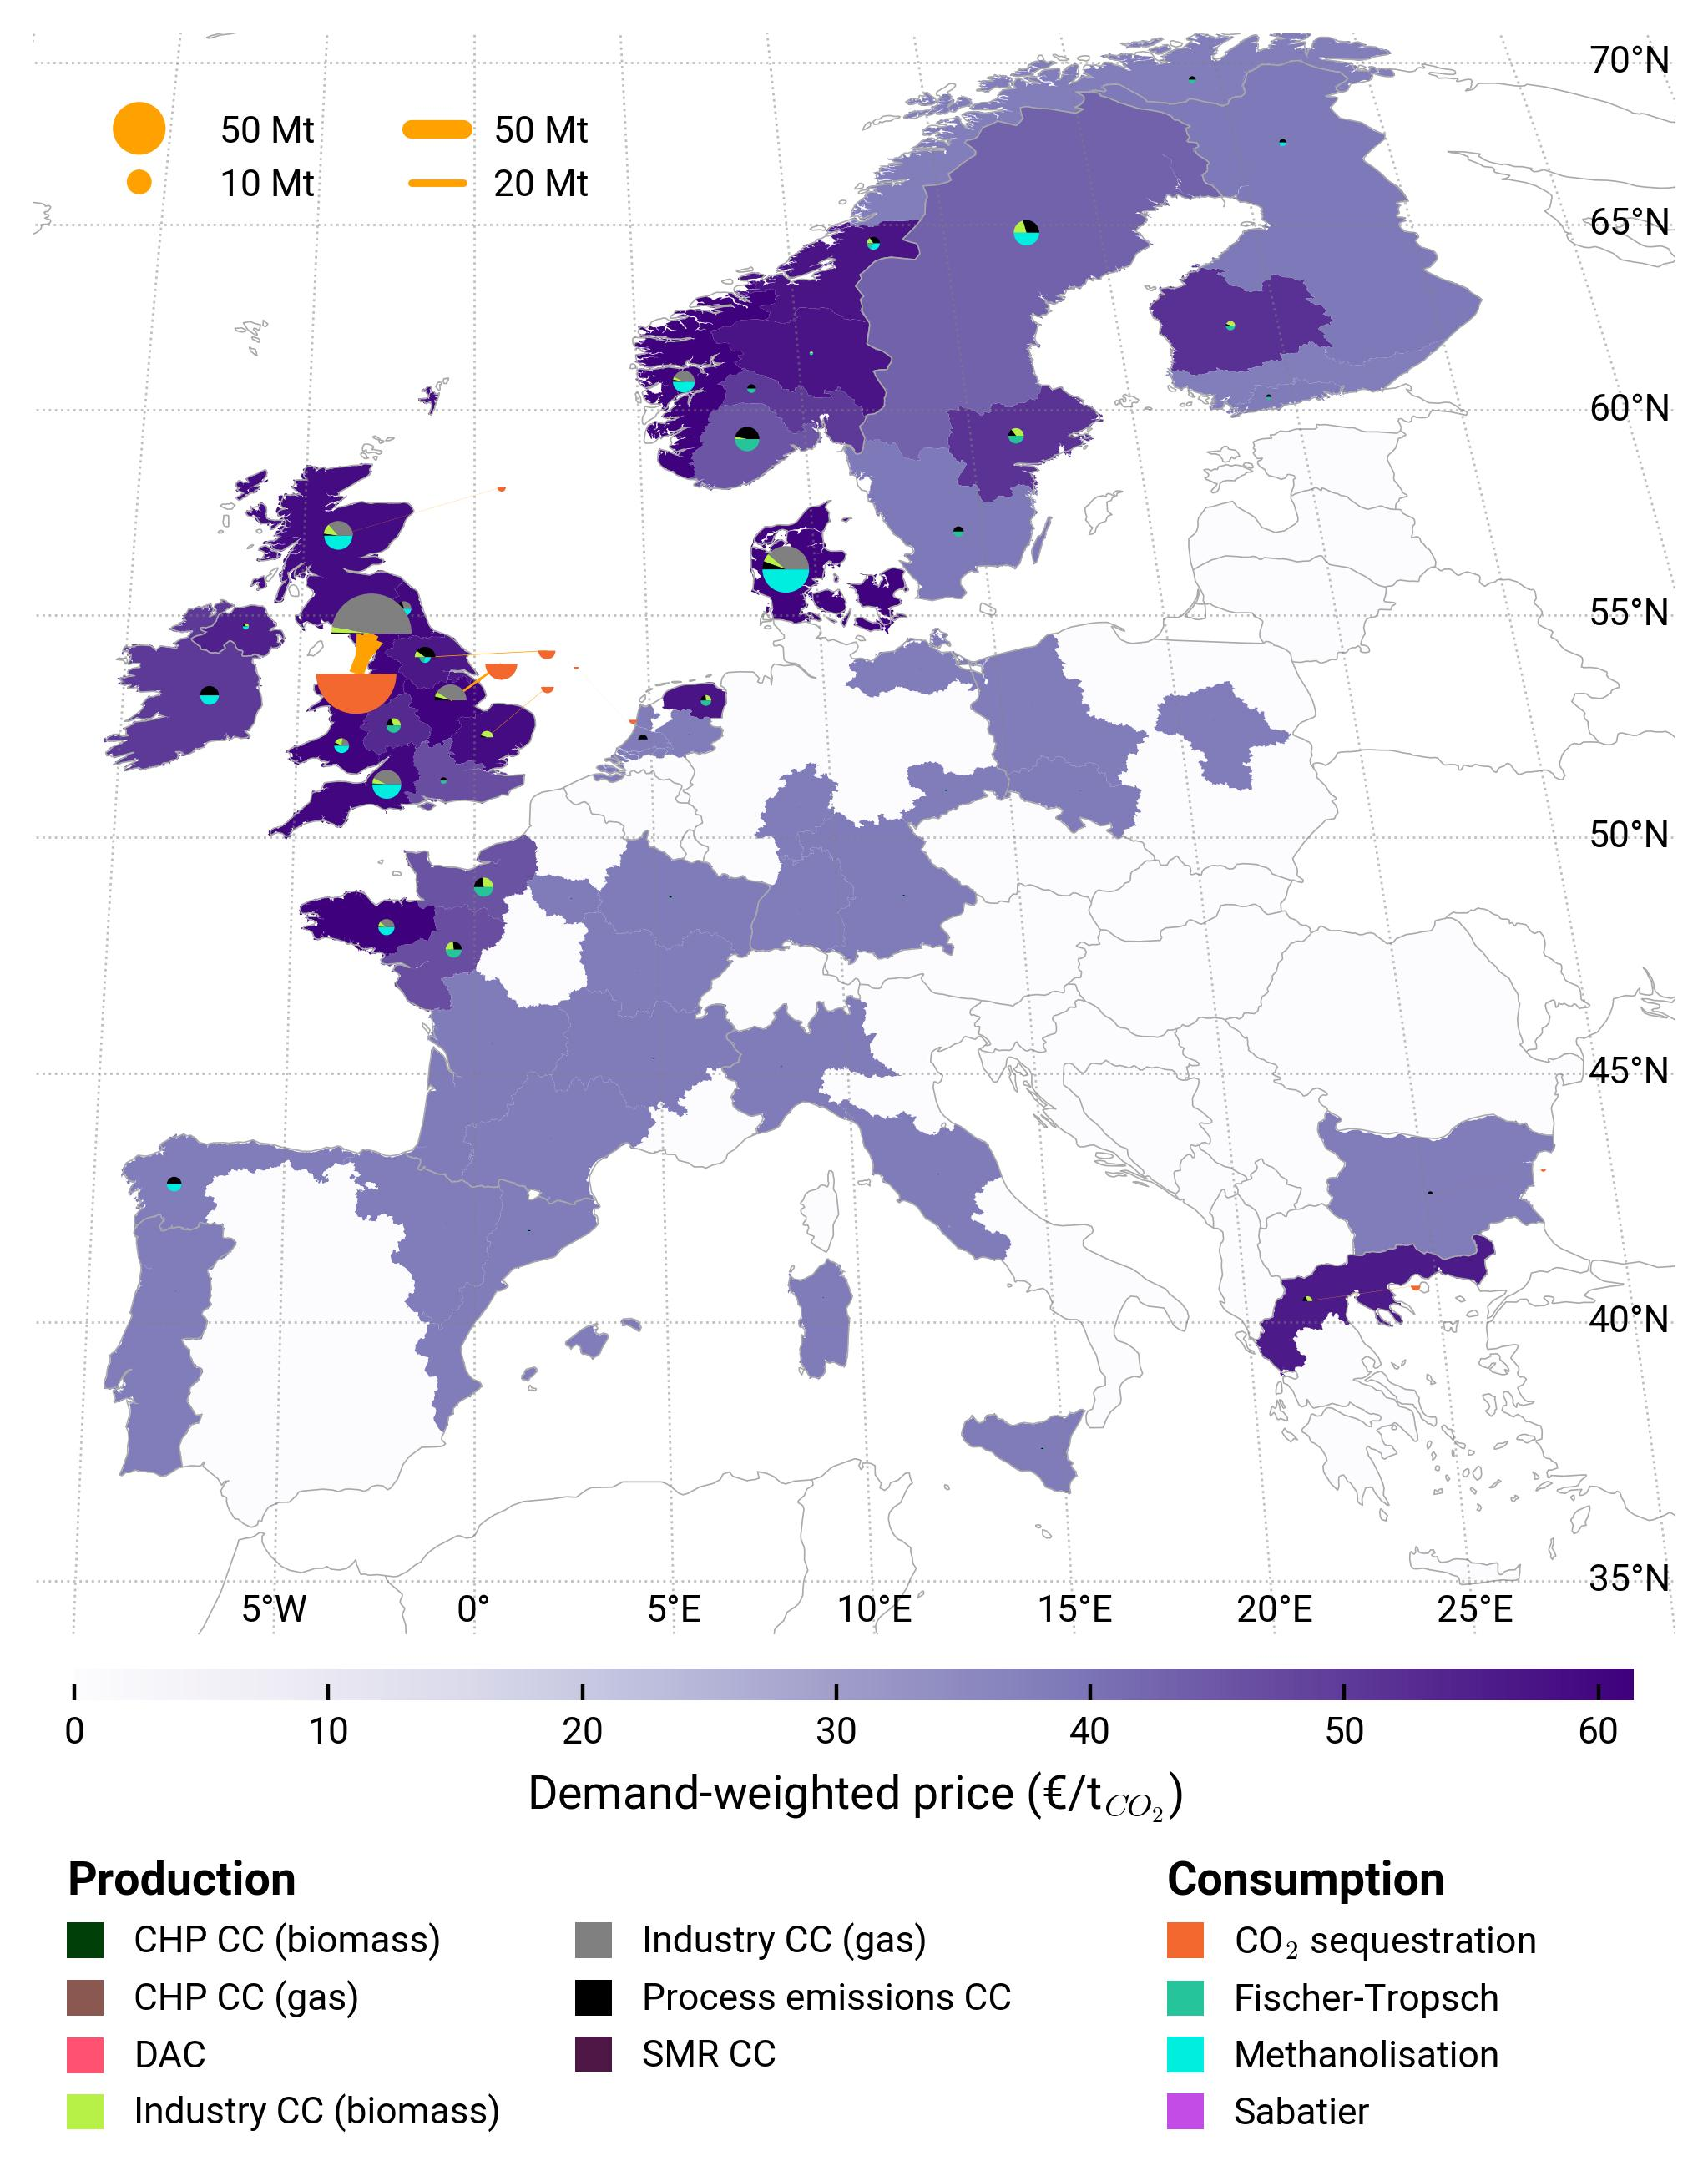
\includegraphics[width=1\textwidth]{maps/no-pipelines-no-pcipmi/base_s_adm___2030-balance_map_co2_stored} 
      \vspace{-0.7cm}
      \caption{\ce{CO2} regional balances and flows.}
      \label{fig:DI_lt_2030_co2}
  \end{subfigure}
  \caption{\textit{Decentral Islands} long-term scenario (2030) --- Regional distribution of \ce{H2} and \ce{CO2} production, utilisation, storage, and transport.}
  \label{fig:DI_lt_2030}
\end{figure*}

\begin{figure*}[htbp]
  \centering
  \begin{subfigure}[t]{0.49\textwidth}
      \vspace{0pt}
      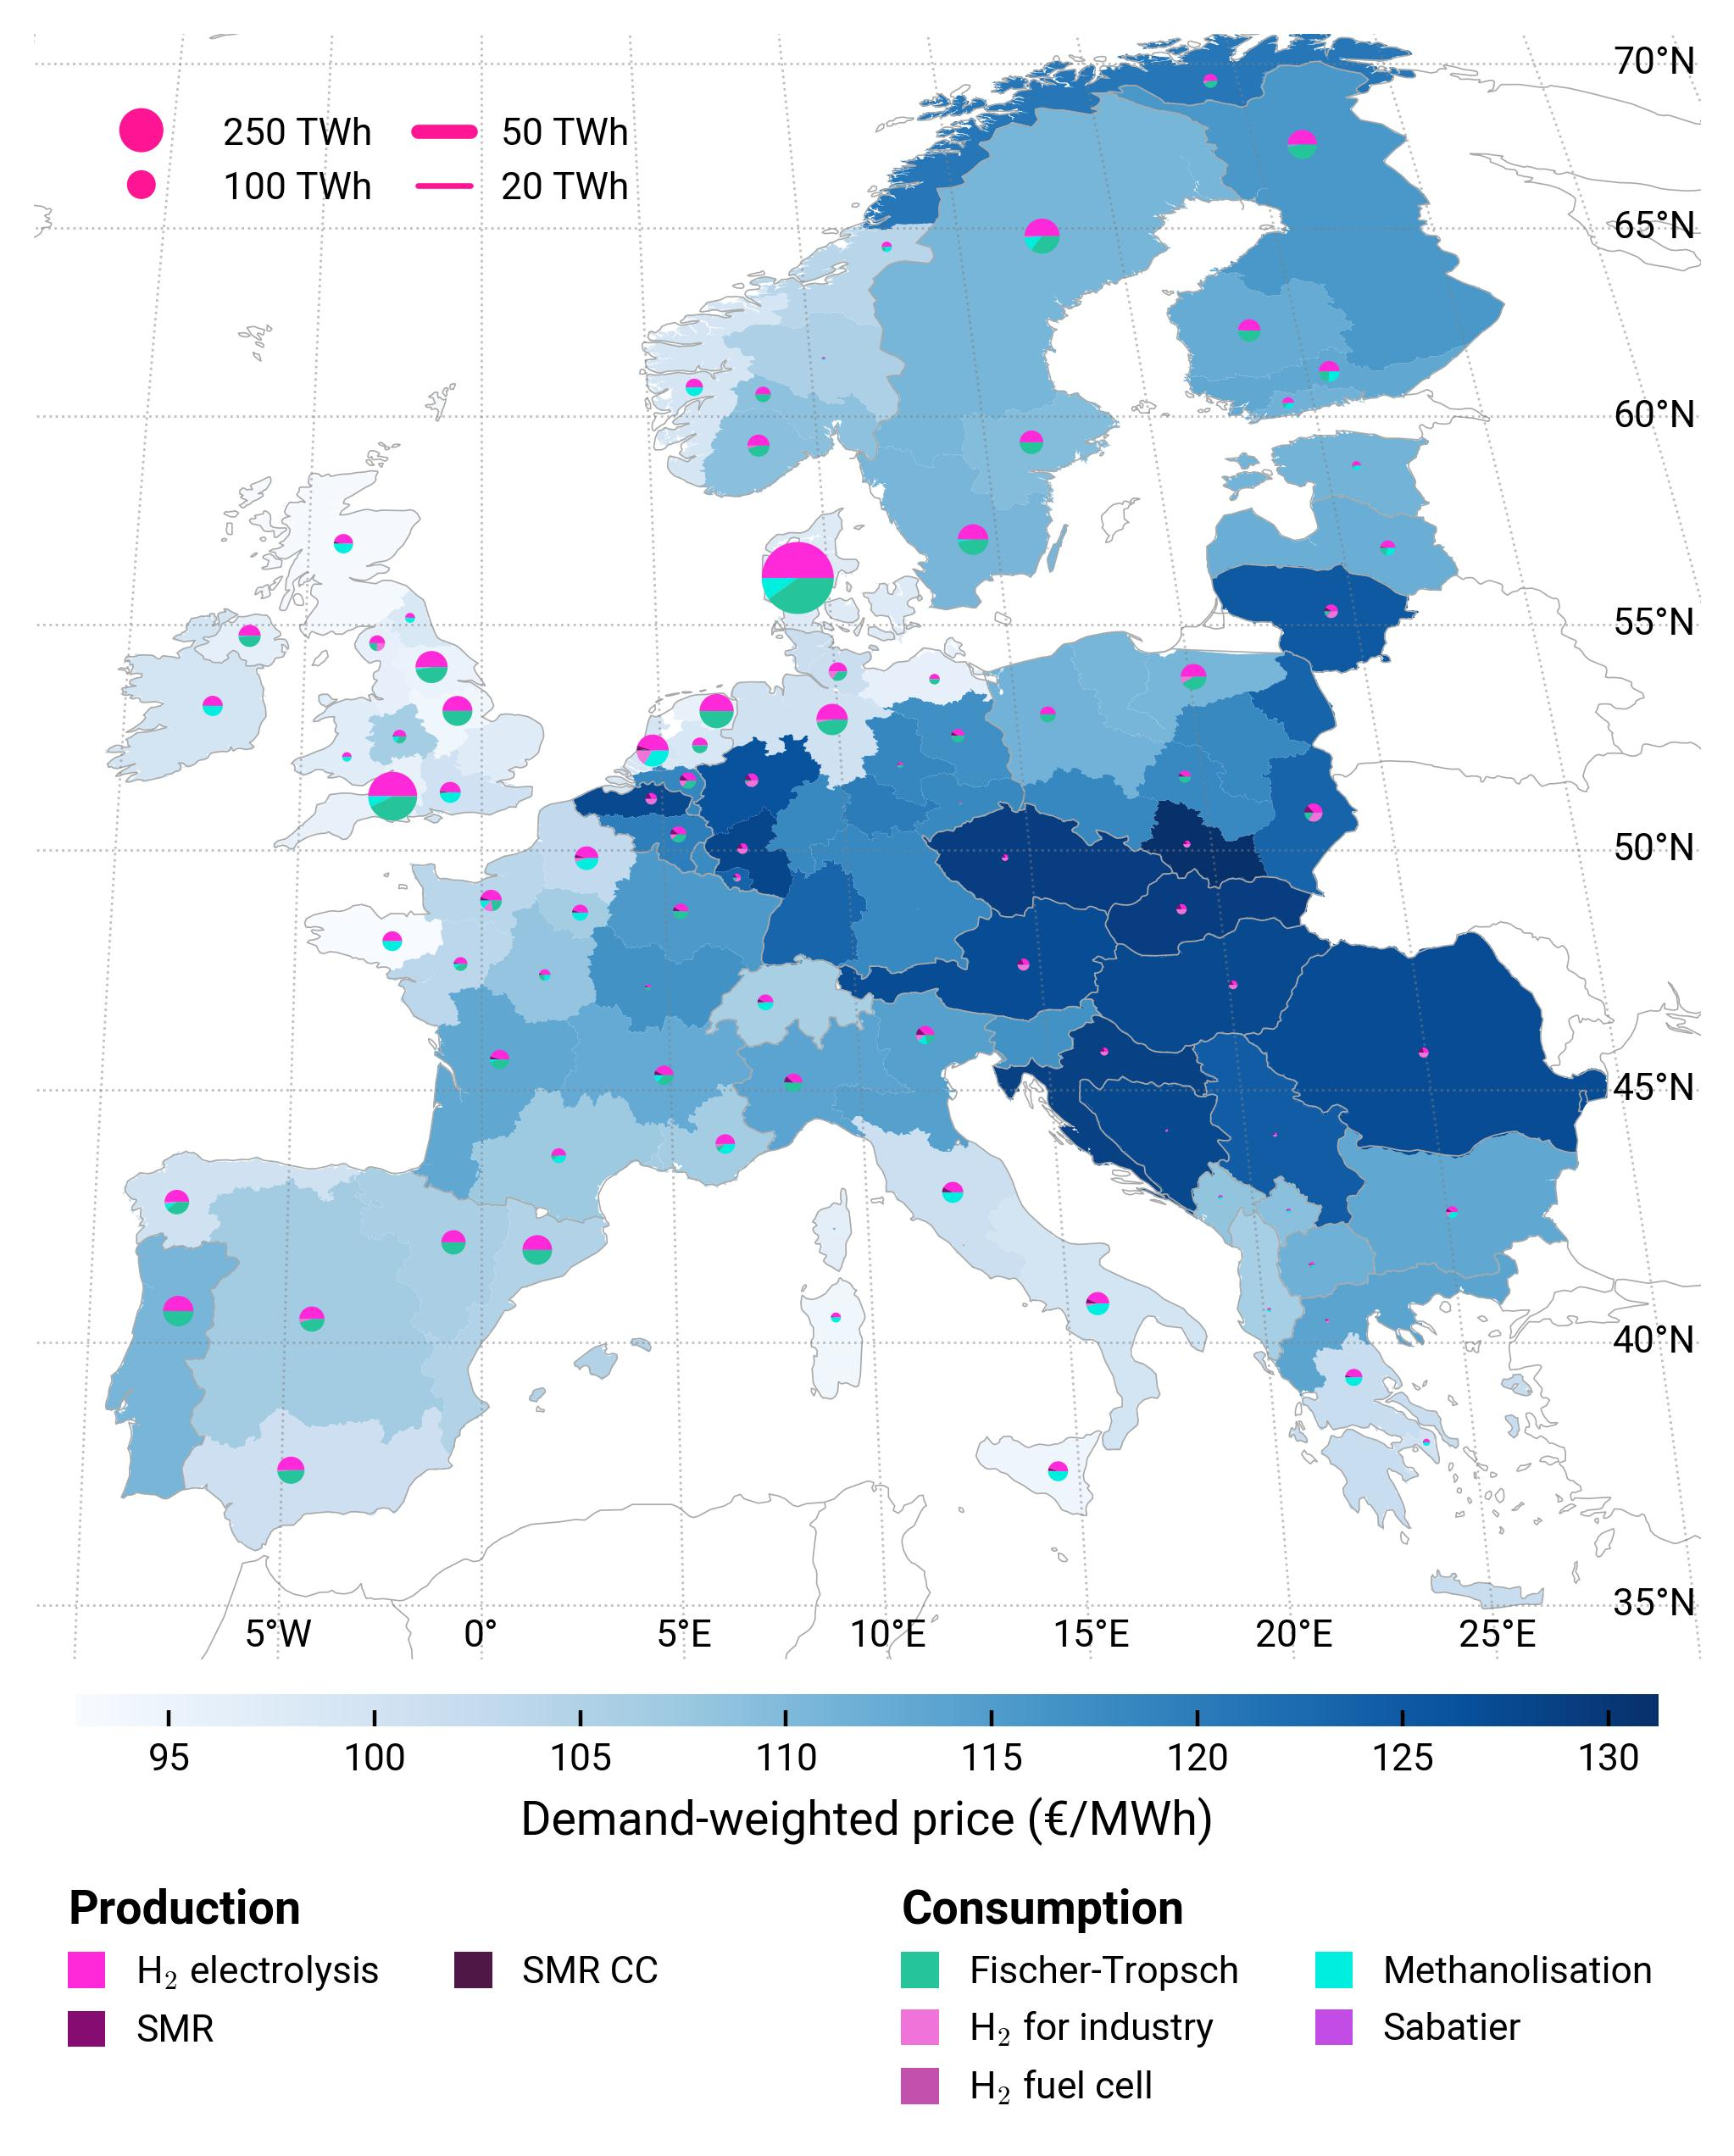
\includegraphics[width=1\textwidth]{maps/no-pipelines-no-pcipmi/base_s_adm___2040-balance_map_H2}
      \vspace{-0.5cm}
      \caption{\ce{H2} regional balances and flows.}
      \label{fig:DI_lt_2040_h2}
  \end{subfigure}
  \hfill
  \begin{subfigure}[t]{0.49\textwidth}
      \vspace{0pt}
      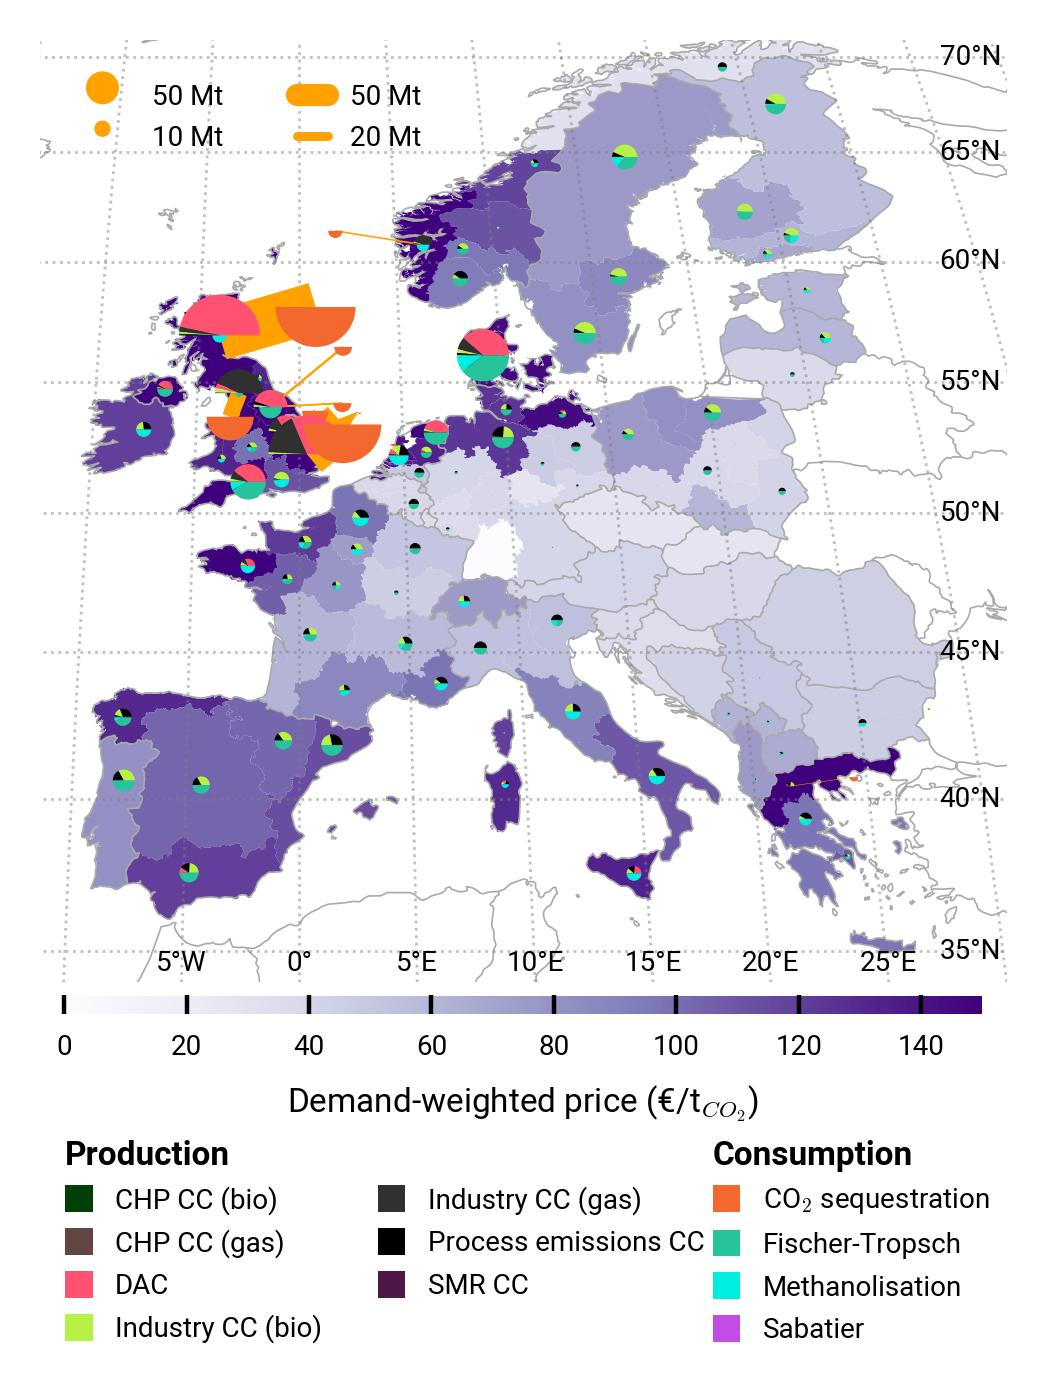
\includegraphics[width=1\textwidth]{maps/no-pipelines-no-pcipmi/base_s_adm___2040-balance_map_co2_stored} 
      \vspace{-0.7cm}
      \caption{\ce{CO2} regional balances and flows.}
      \label{fig:DI_lt_2040_co2}
  \end{subfigure}
  \caption{\textit{Decentral Islands} long-term scenario (2040) --- Regional distribution of \ce{H2} and \ce{CO2} production, utilisation, storage, and transport.}
  \label{fig:DI_lt_2040}
\end{figure*}

\begin{figure*}[htbp]
  \centering
  \begin{subfigure}[t]{0.49\textwidth}
      \vspace{0pt}
      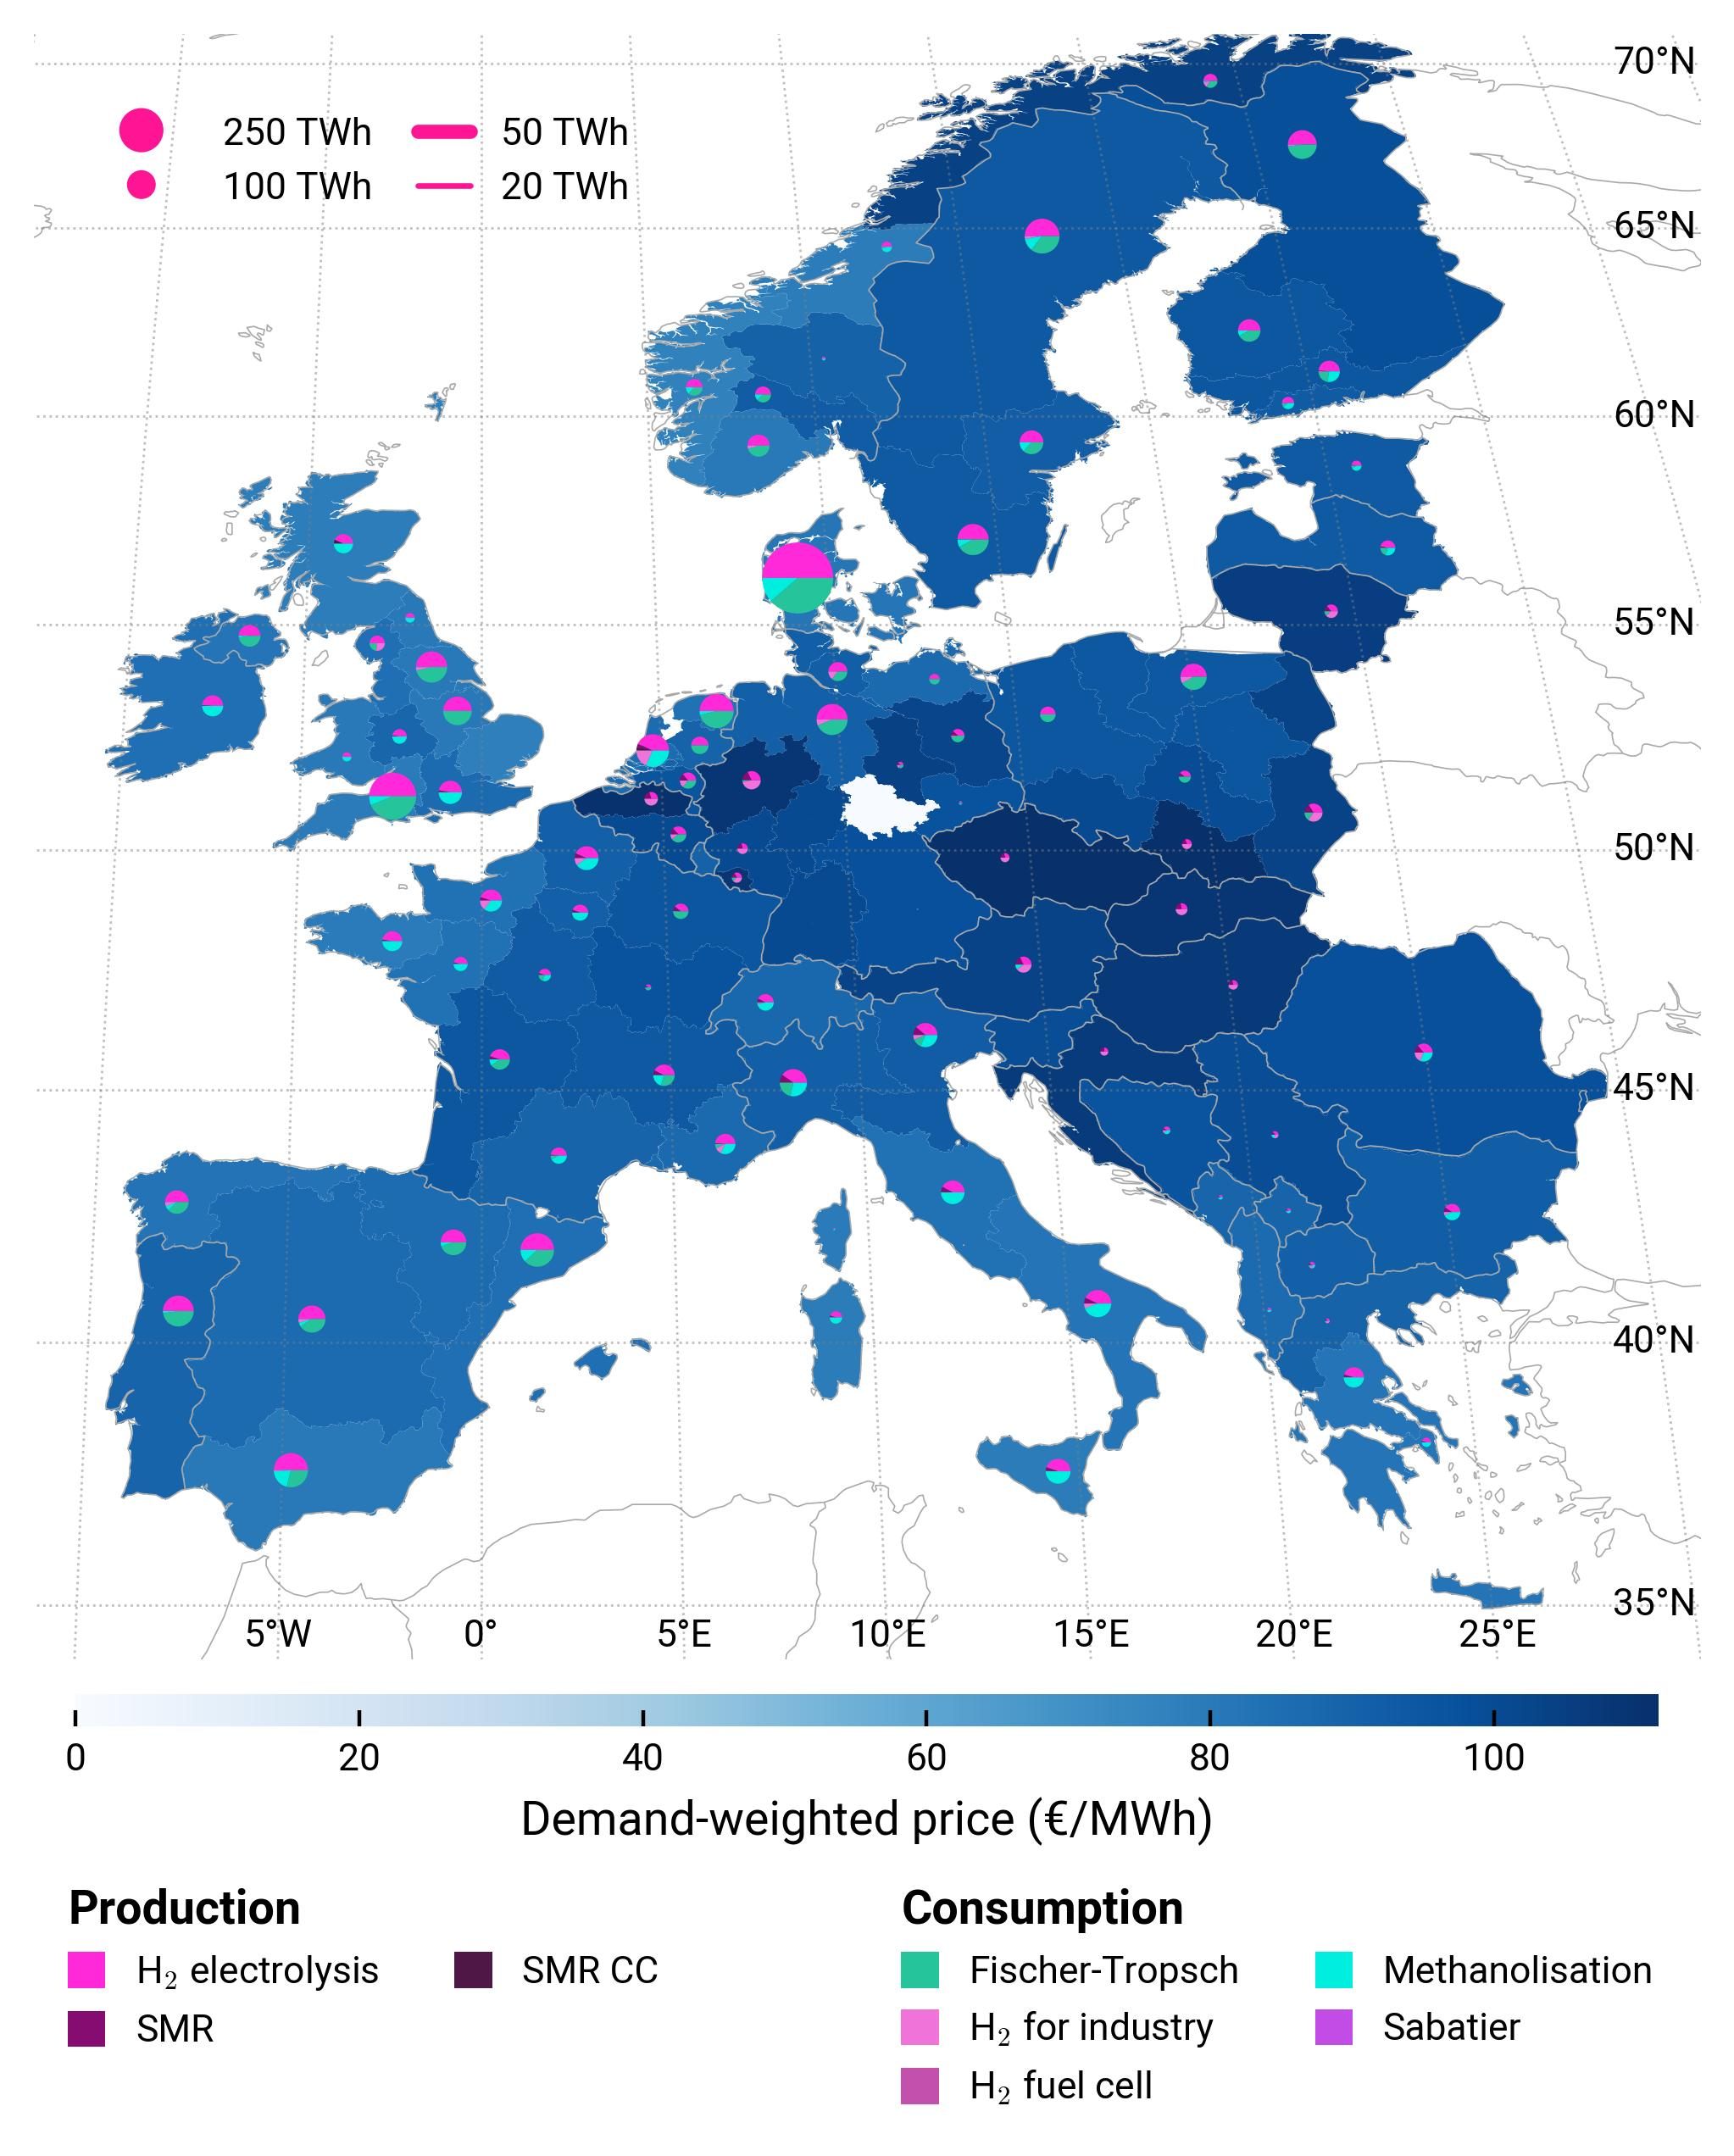
\includegraphics[width=1\textwidth]{maps/no-pipelines-no-pcipmi/base_s_adm___2050-balance_map_H2}
      \vspace{-0.5cm}
      \caption{\ce{H2} regional balances and flows.}
      \label{fig:DI_lt_2050_h2}
  \end{subfigure}
  \hfill
  \begin{subfigure}[t]{0.49\textwidth}
      \vspace{0pt}
      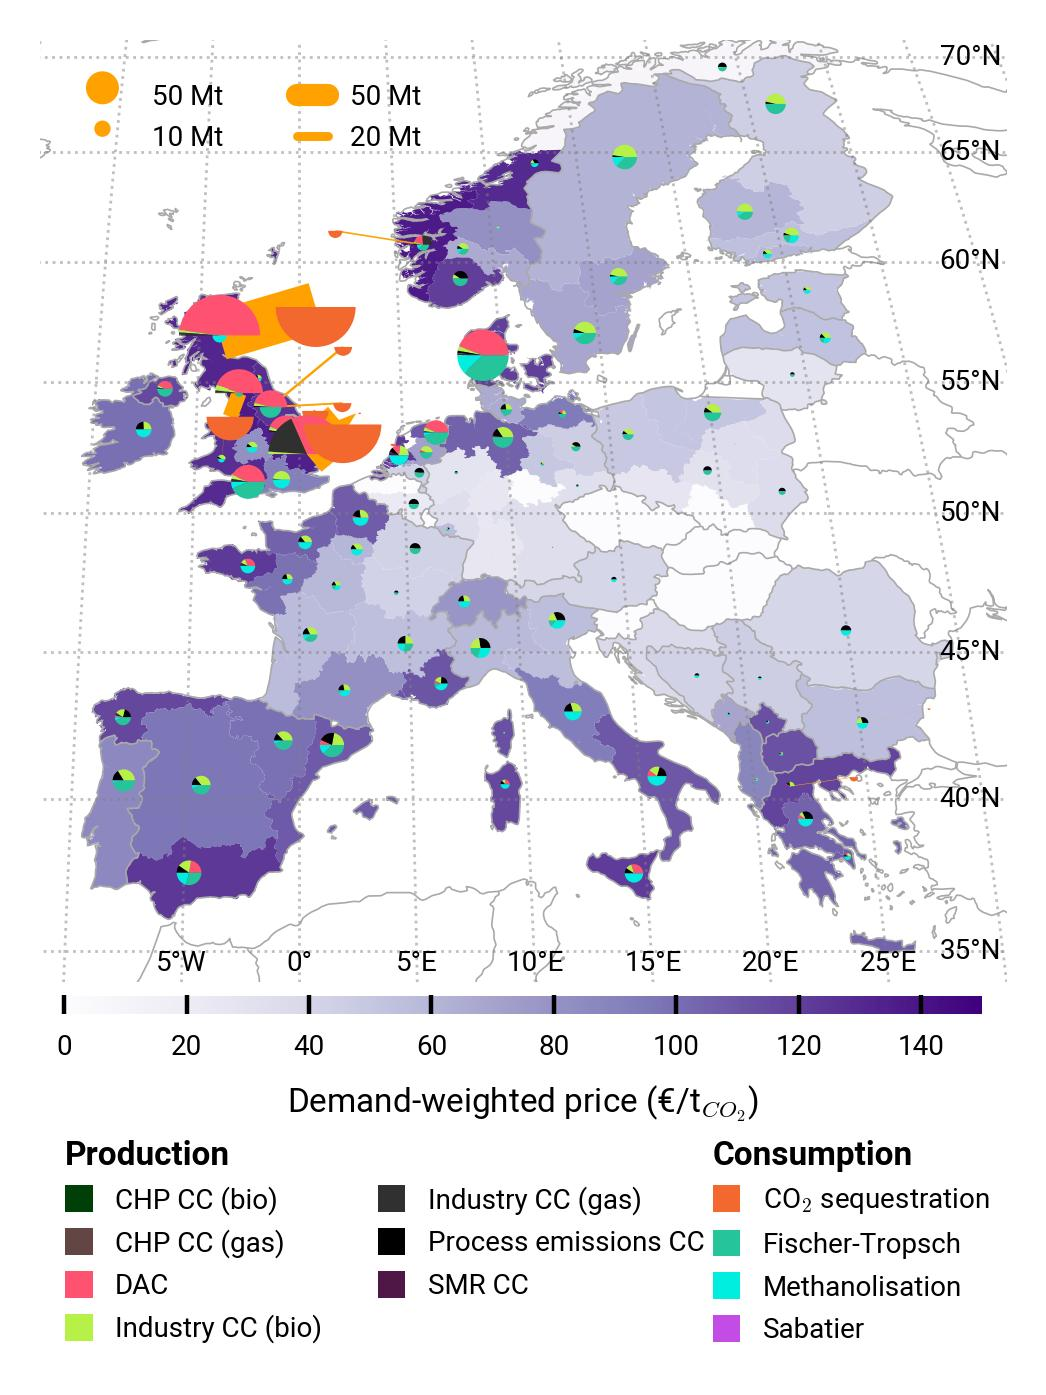
\includegraphics[width=1\textwidth]{maps/no-pipelines-no-pcipmi/base_s_adm___2050-balance_map_co2_stored} 
      \vspace{-0.7cm}
      \caption{\ce{CO2} regional balances and flows.}
      \label{fig:DI_lt_2050_co2}
  \end{subfigure}
  \caption{\textit{Decentral Islands} long-term scenario (2050) --- Regional distribution of \ce{H2} and \ce{CO2} production, utilisation, storage, and transport.}
  \label{fig:DI_lt_2050}
\end{figure*}

\clearpage

\subsection{PCI international}

\begin{figure*}[htbp]
  \centering
  \begin{subfigure}[t]{0.49\textwidth}
      \vspace{0pt}
      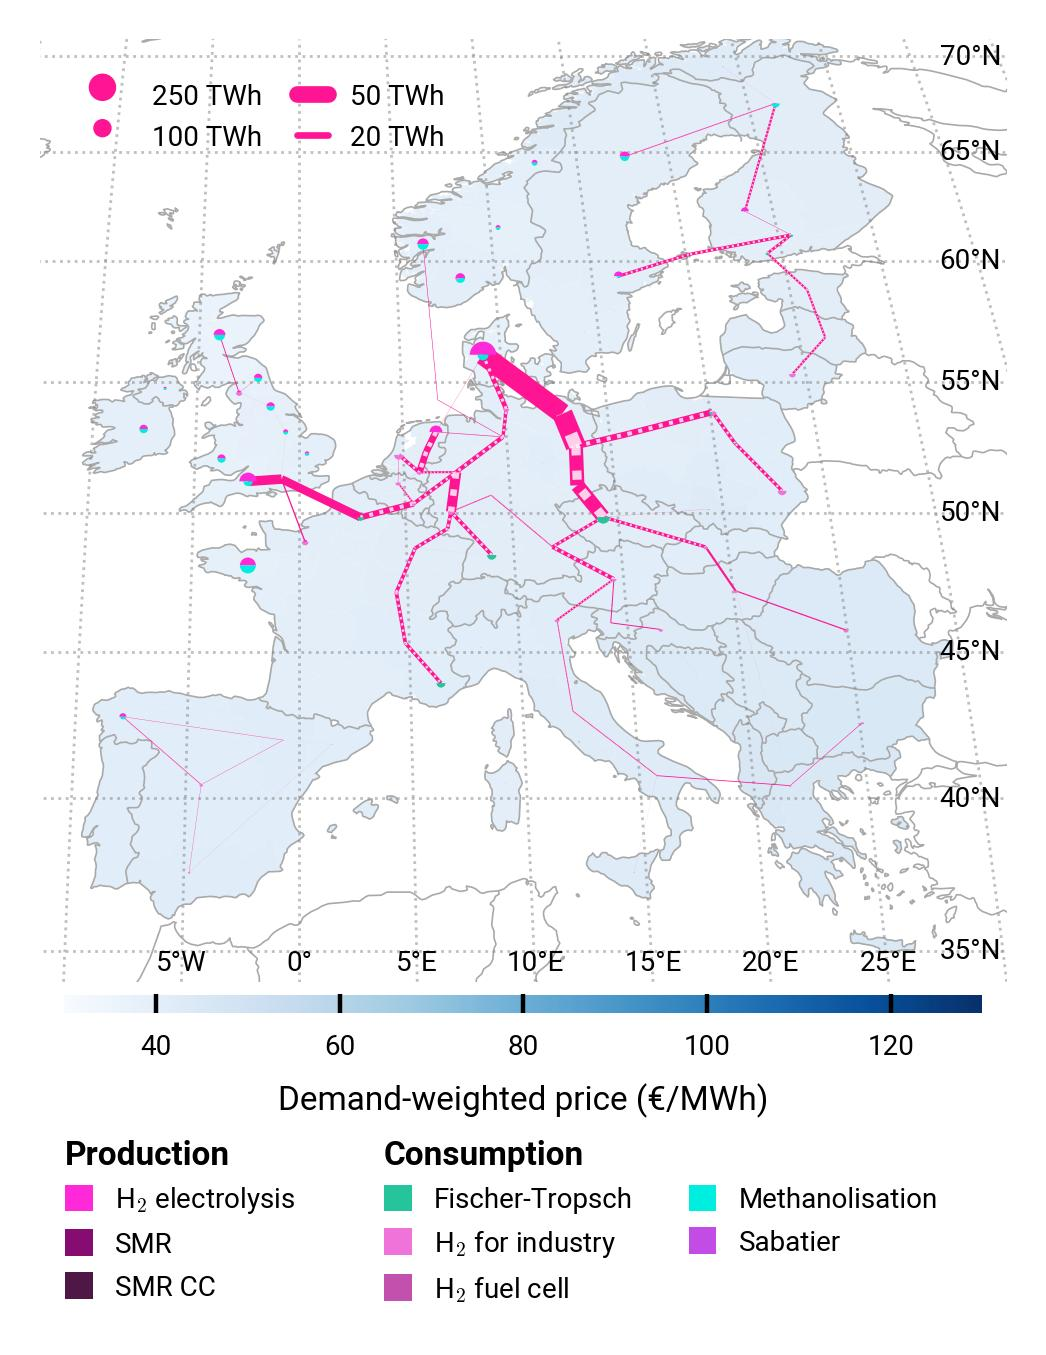
\includegraphics[width=1\textwidth]{maps/pcipmi-national-international-expansion/base_s_adm___2030-balance_map_H2}
      \vspace{-0.5cm}
      \caption{\ce{H2} regional balances and flows.}
      \label{fig:PCI-in_lt_2030_h2}
  \end{subfigure}
  \hfill
  \begin{subfigure}[t]{0.49\textwidth}
      \vspace{0pt}
      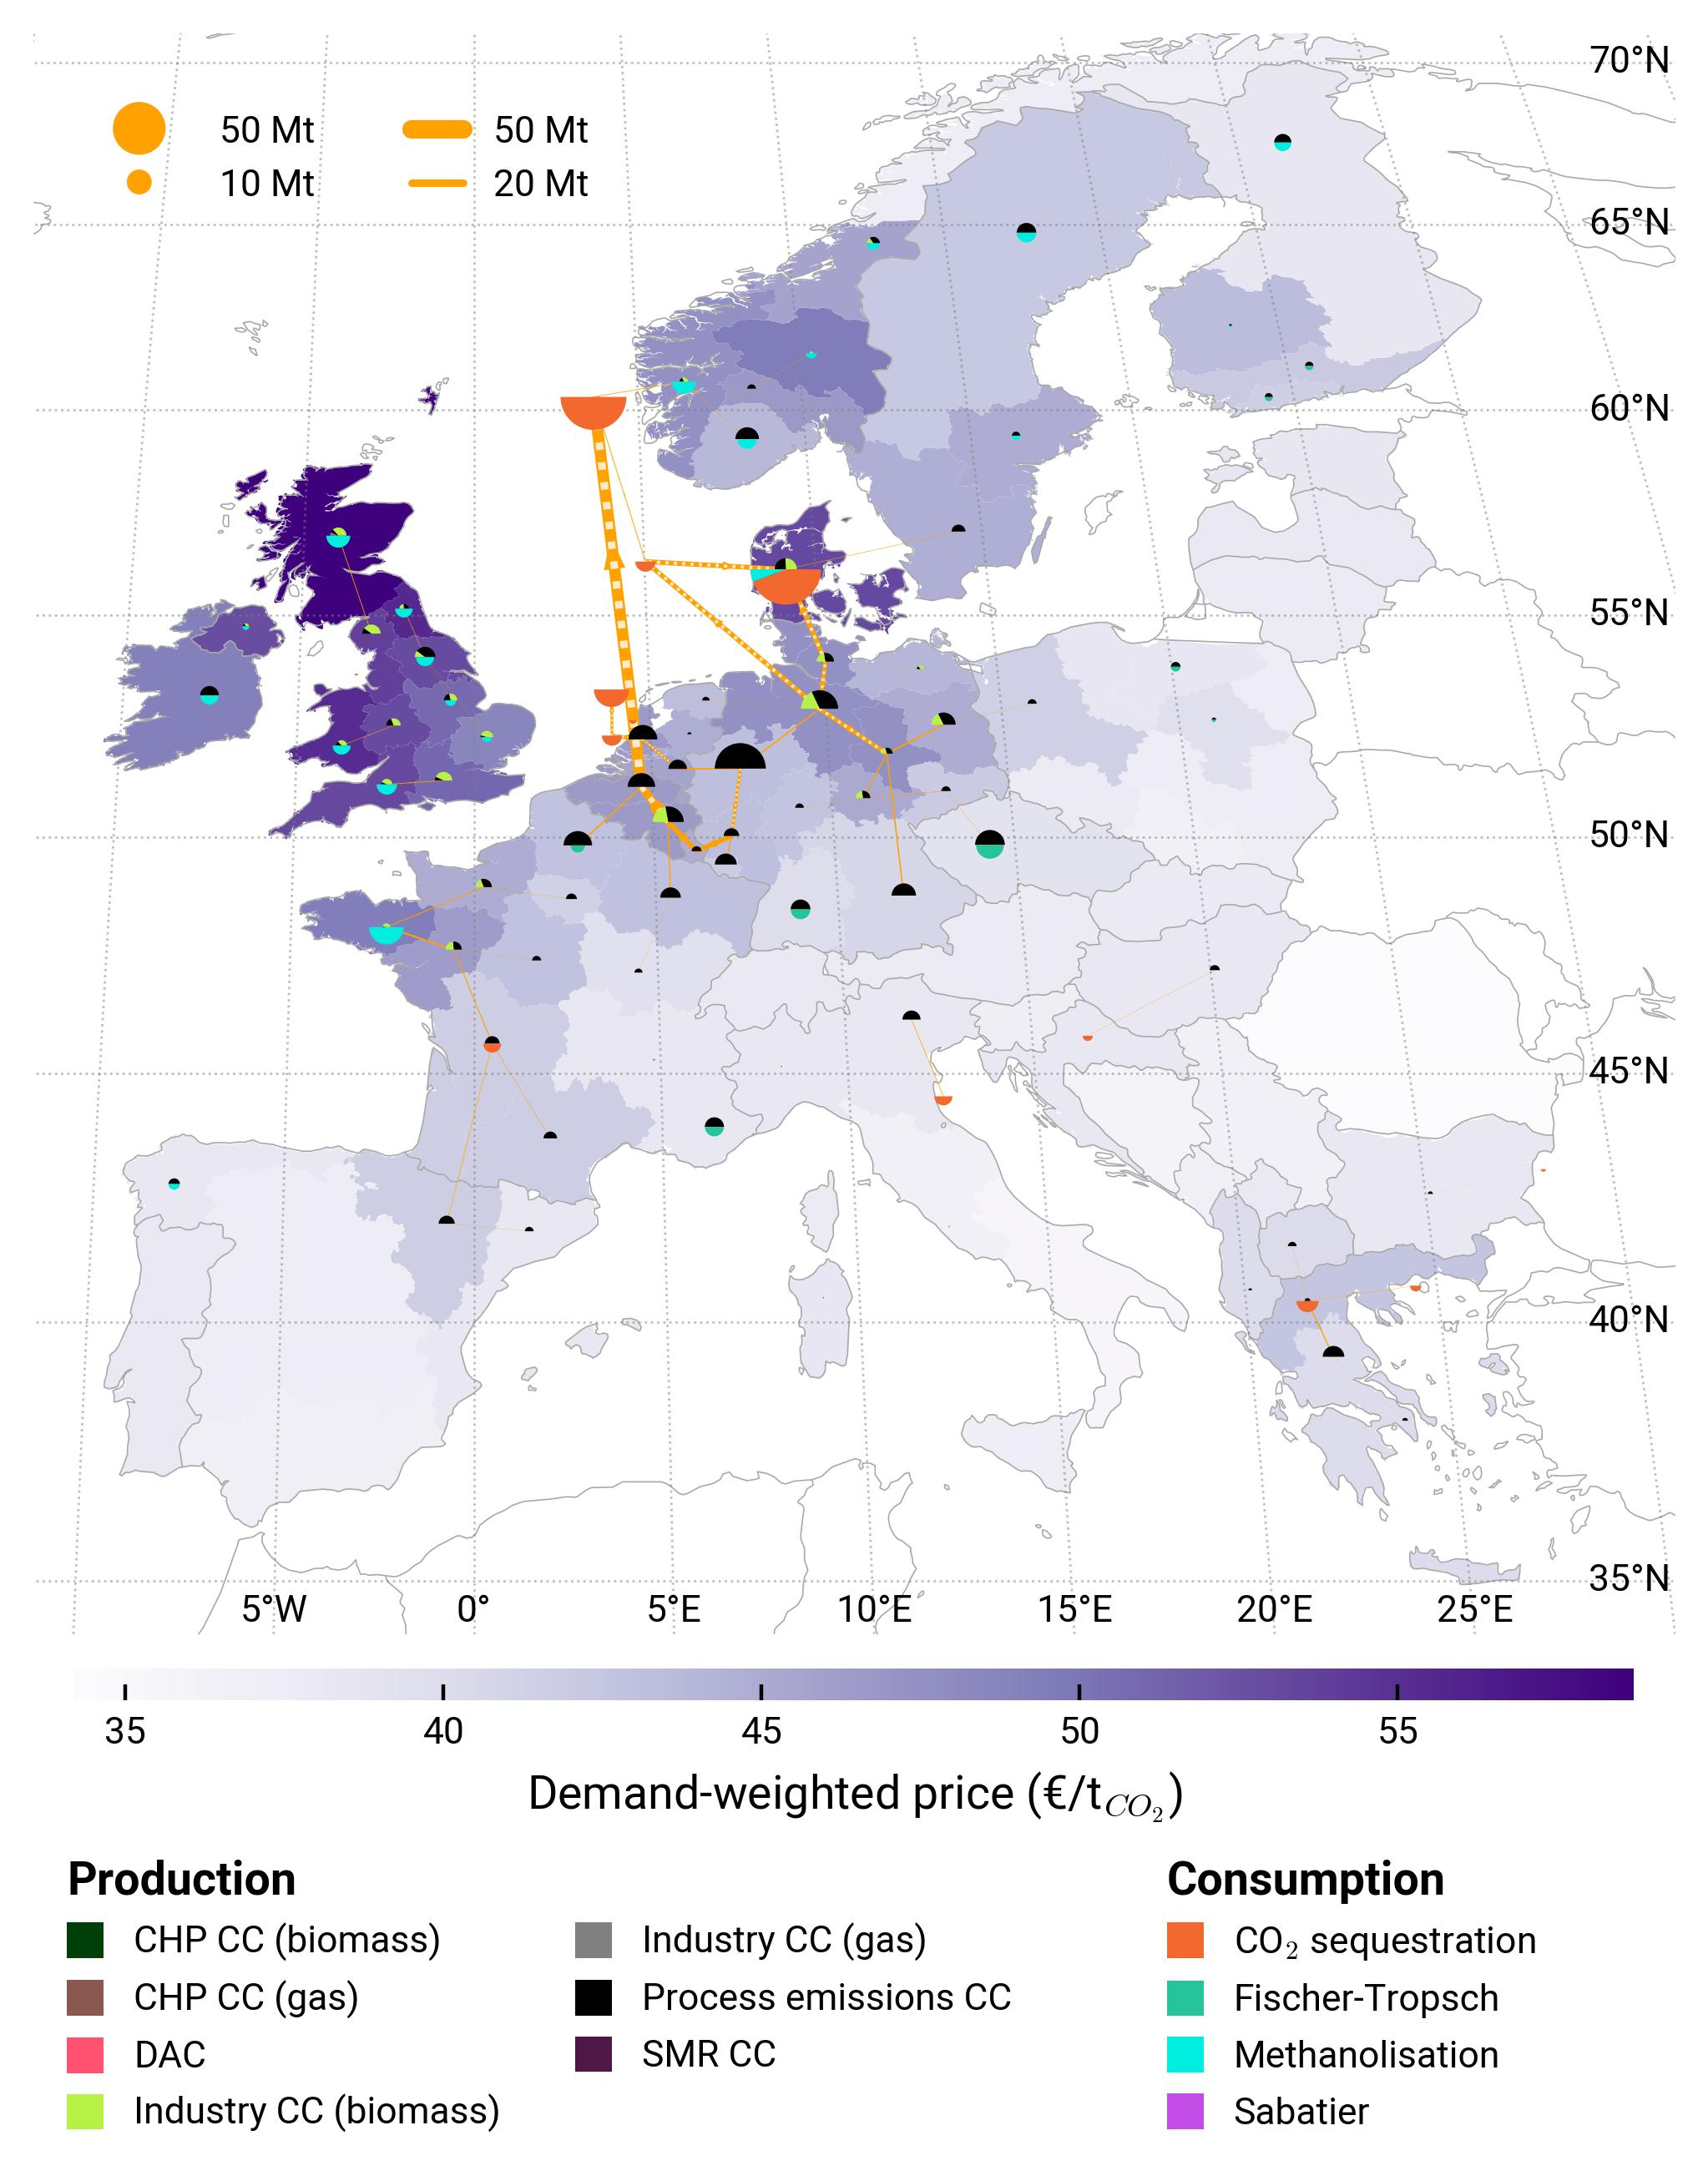
\includegraphics[width=1\textwidth]{maps/pcipmi-national-international-expansion/base_s_adm___2030-balance_map_co2_stored} 
      \vspace{-0.7cm}
      \caption{\ce{CO2} regional balances and flows.}
      \label{fig:PCI-in_lt_2030_co2}
  \end{subfigure}
  \caption{\textit{PCI} long-term scenario (2030) --- Regional distribution of \ce{H2} and \ce{CO2} production, utilisation, storage, and transport. Dotted white lines represent PCI-PMI projects.}
  \label{fig:PCI-in_lt_2030}
\end{figure*}

\begin{figure*}[htbp]
  \centering
  \begin{subfigure}[t]{0.49\textwidth}
      \vspace{0pt}
      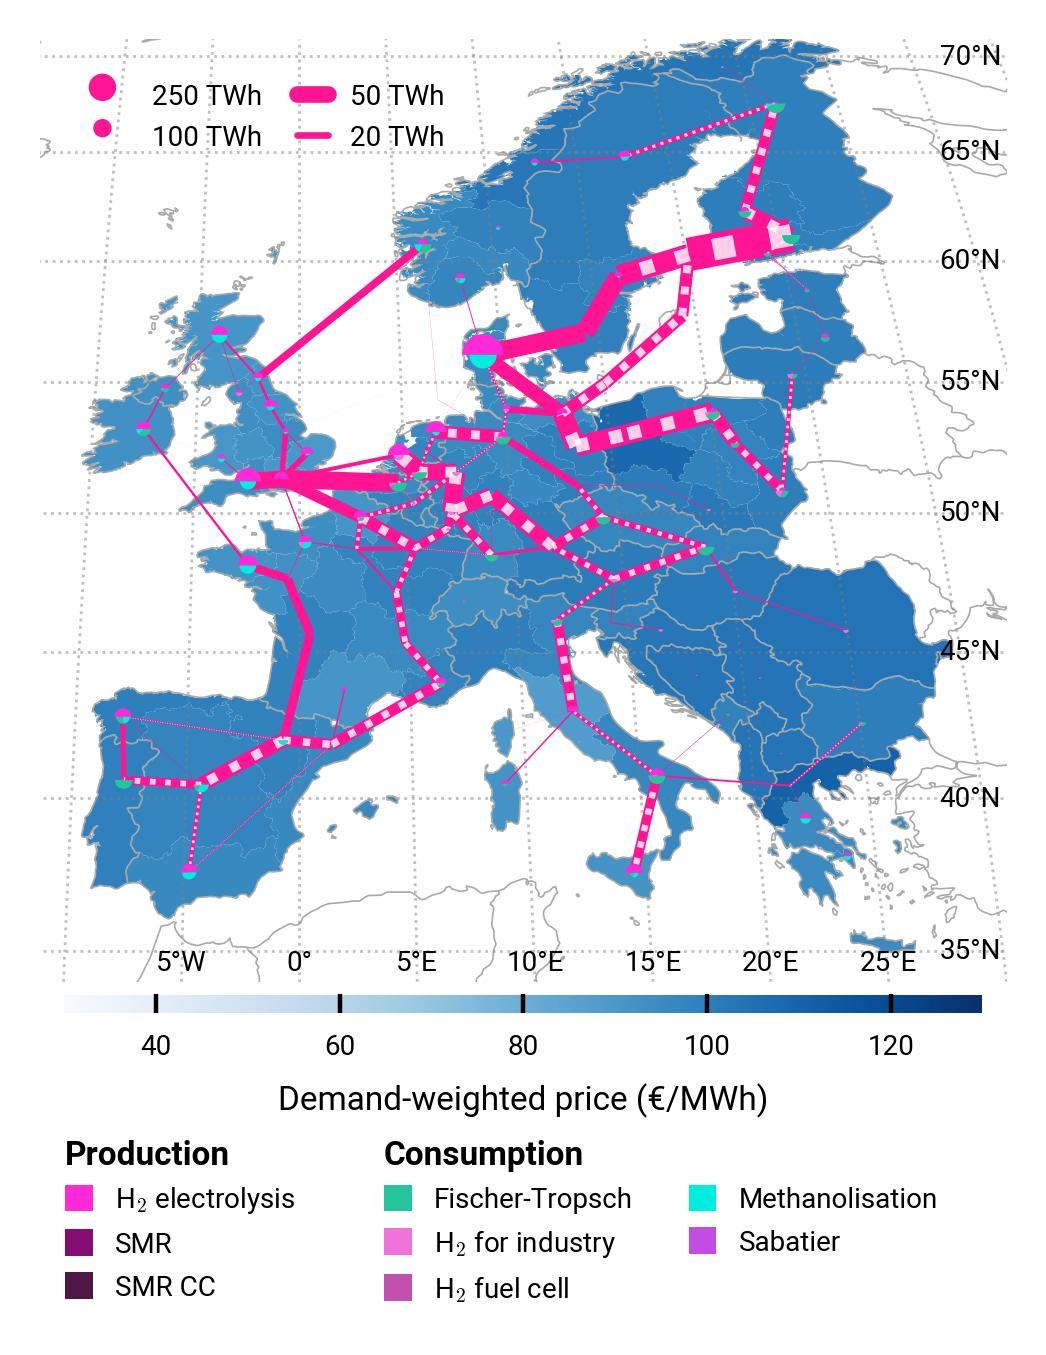
\includegraphics[width=1\textwidth]{maps/pcipmi-national-international-expansion/base_s_adm___2040-balance_map_H2}
      \vspace{-0.5cm}
      \caption{\ce{H2} regional balances and flows.}
      \label{fig:PCI-in_lt_2040_h2}
  \end{subfigure}
  \hfill
  \begin{subfigure}[t]{0.49\textwidth}
      \vspace{0pt}
      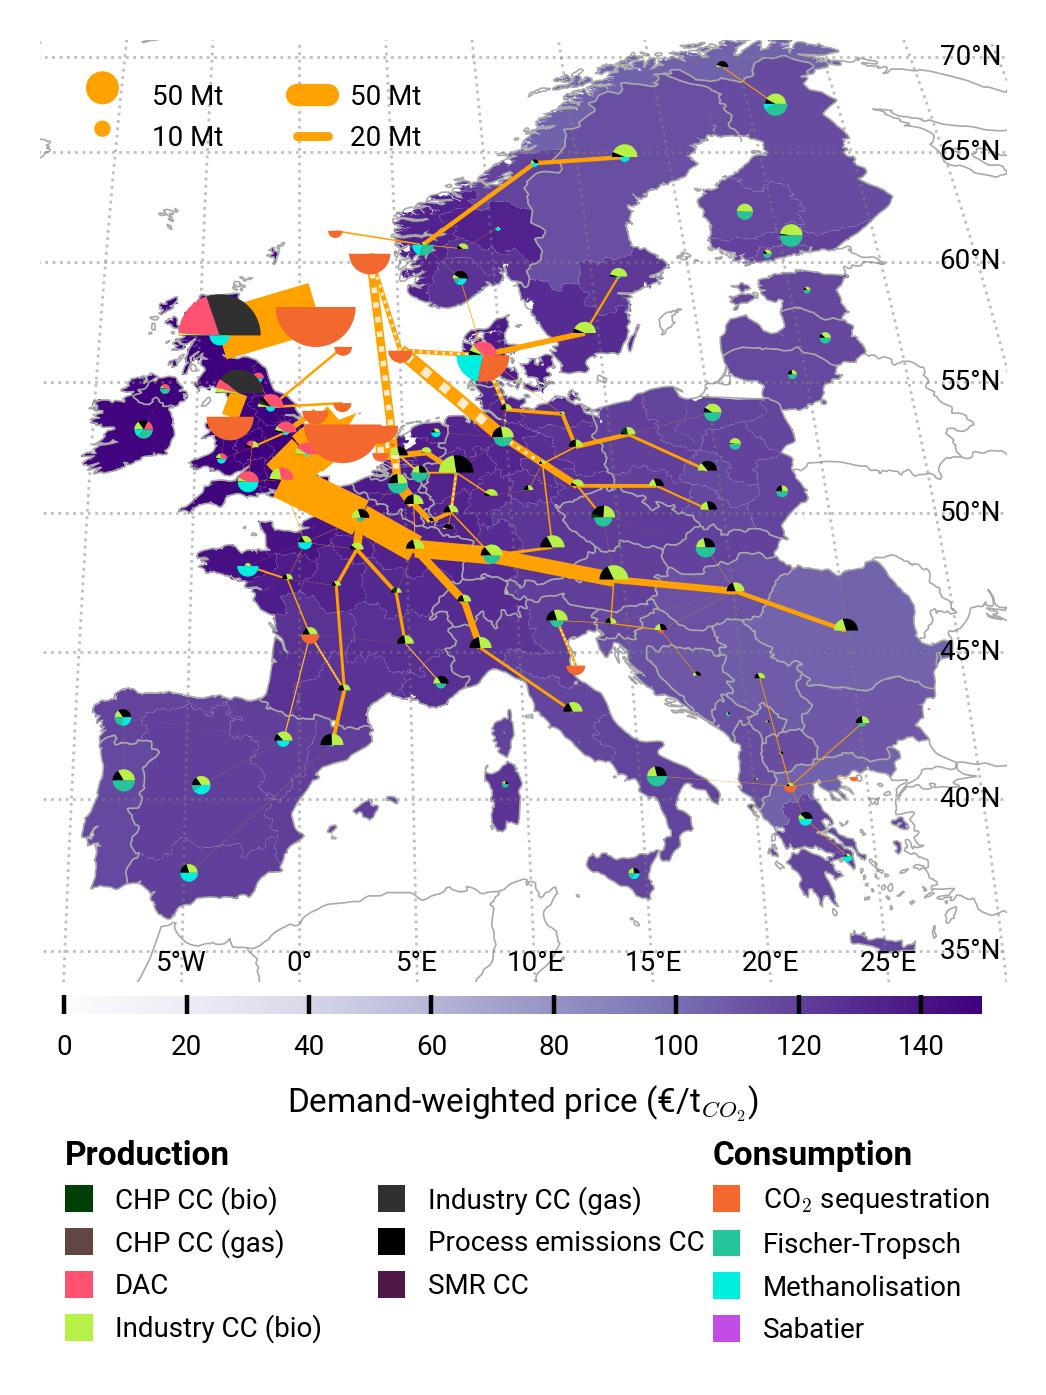
\includegraphics[width=1\textwidth]{maps/pcipmi-national-international-expansion/base_s_adm___2040-balance_map_co2_stored} 
      \vspace{-0.7cm}
      \caption{\ce{CO2} regional balances and flows.}
      \label{fig:PCI-in_lt_2040_co2}
  \end{subfigure}
  \caption{\textit{PCI-in} long-term scenario (2040) --- Regional distribution of \ce{H2} and \ce{CO2} production, utilisation, storage, and transport. Dotted white lines represent PCI-PMI projects.}
  \label{fig:PCI-in_lt_2040}
\end{figure*}

\begin{figure*}[htbp]
  \centering
  \begin{subfigure}[t]{0.49\textwidth}
      \vspace{0pt}
      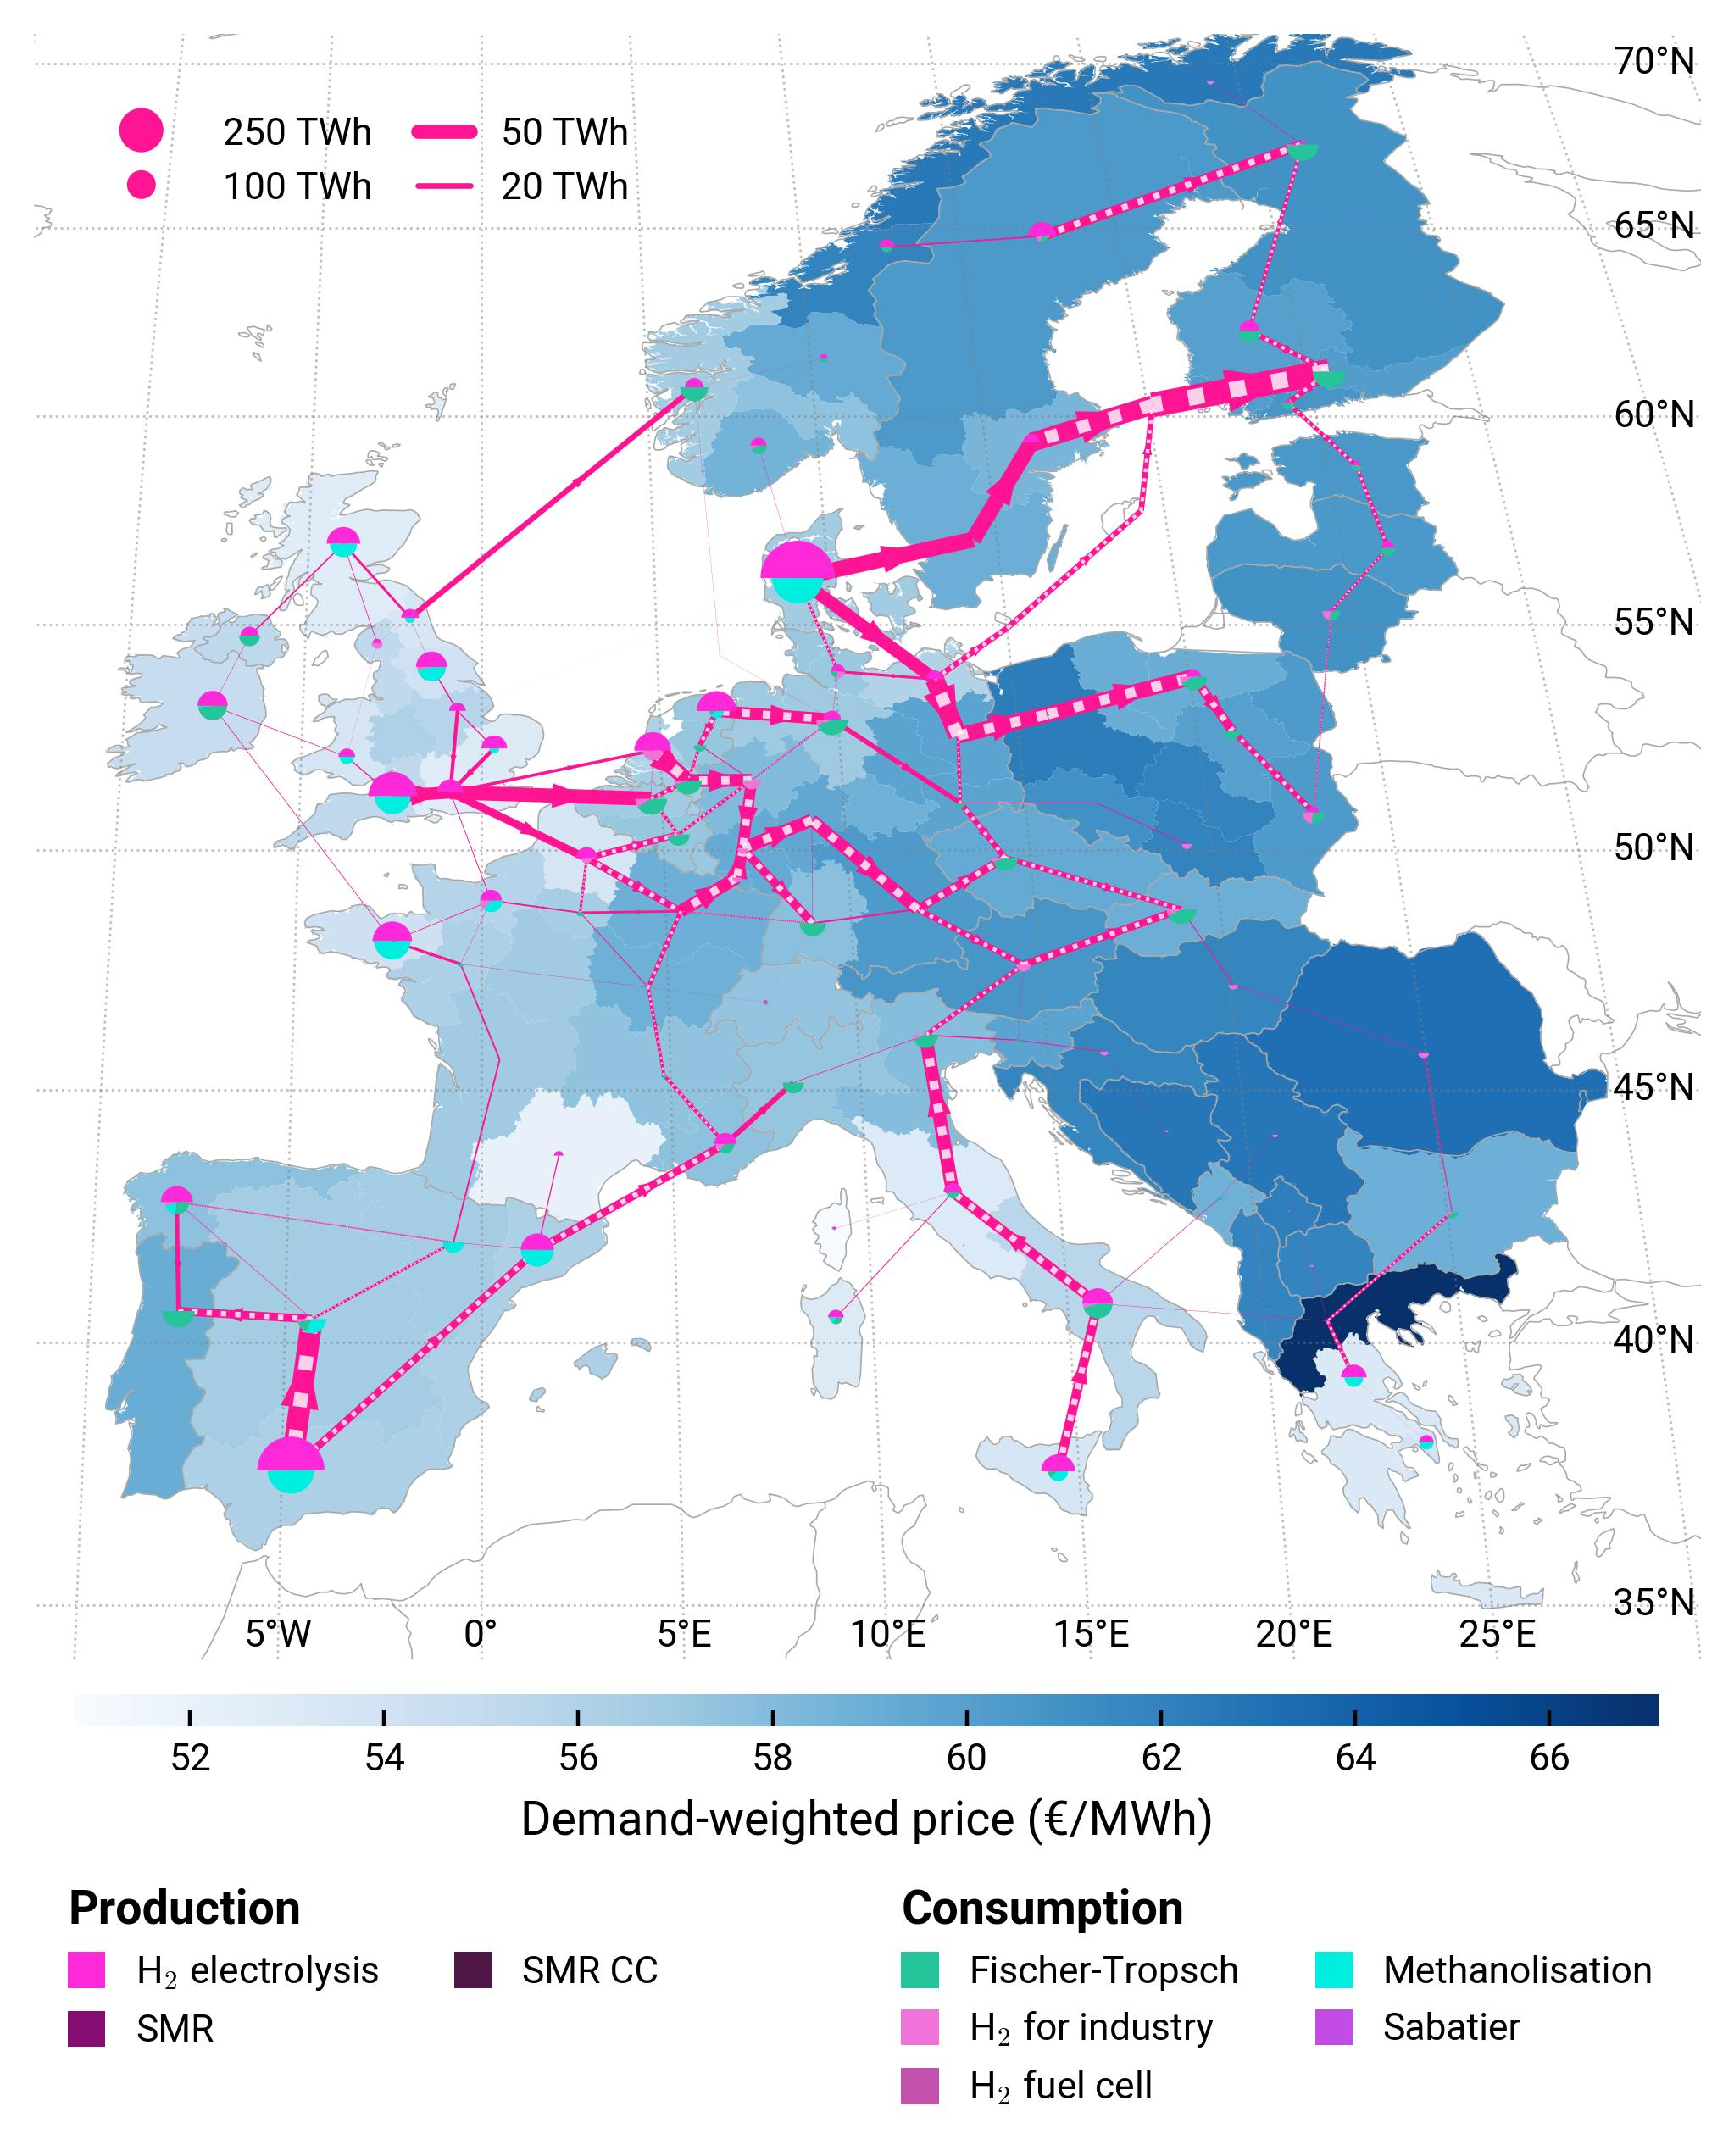
\includegraphics[width=1\textwidth]{maps/pcipmi-national-international-expansion/base_s_adm___2050-balance_map_H2}
      \vspace{-0.5cm}
      \caption{\ce{H2} regional balances and flows.}
      \label{fig:PCI-in_lt_2050_h2}
  \end{subfigure}
  \hfill
  \begin{subfigure}[t]{0.49\textwidth}
      \vspace{0pt}
      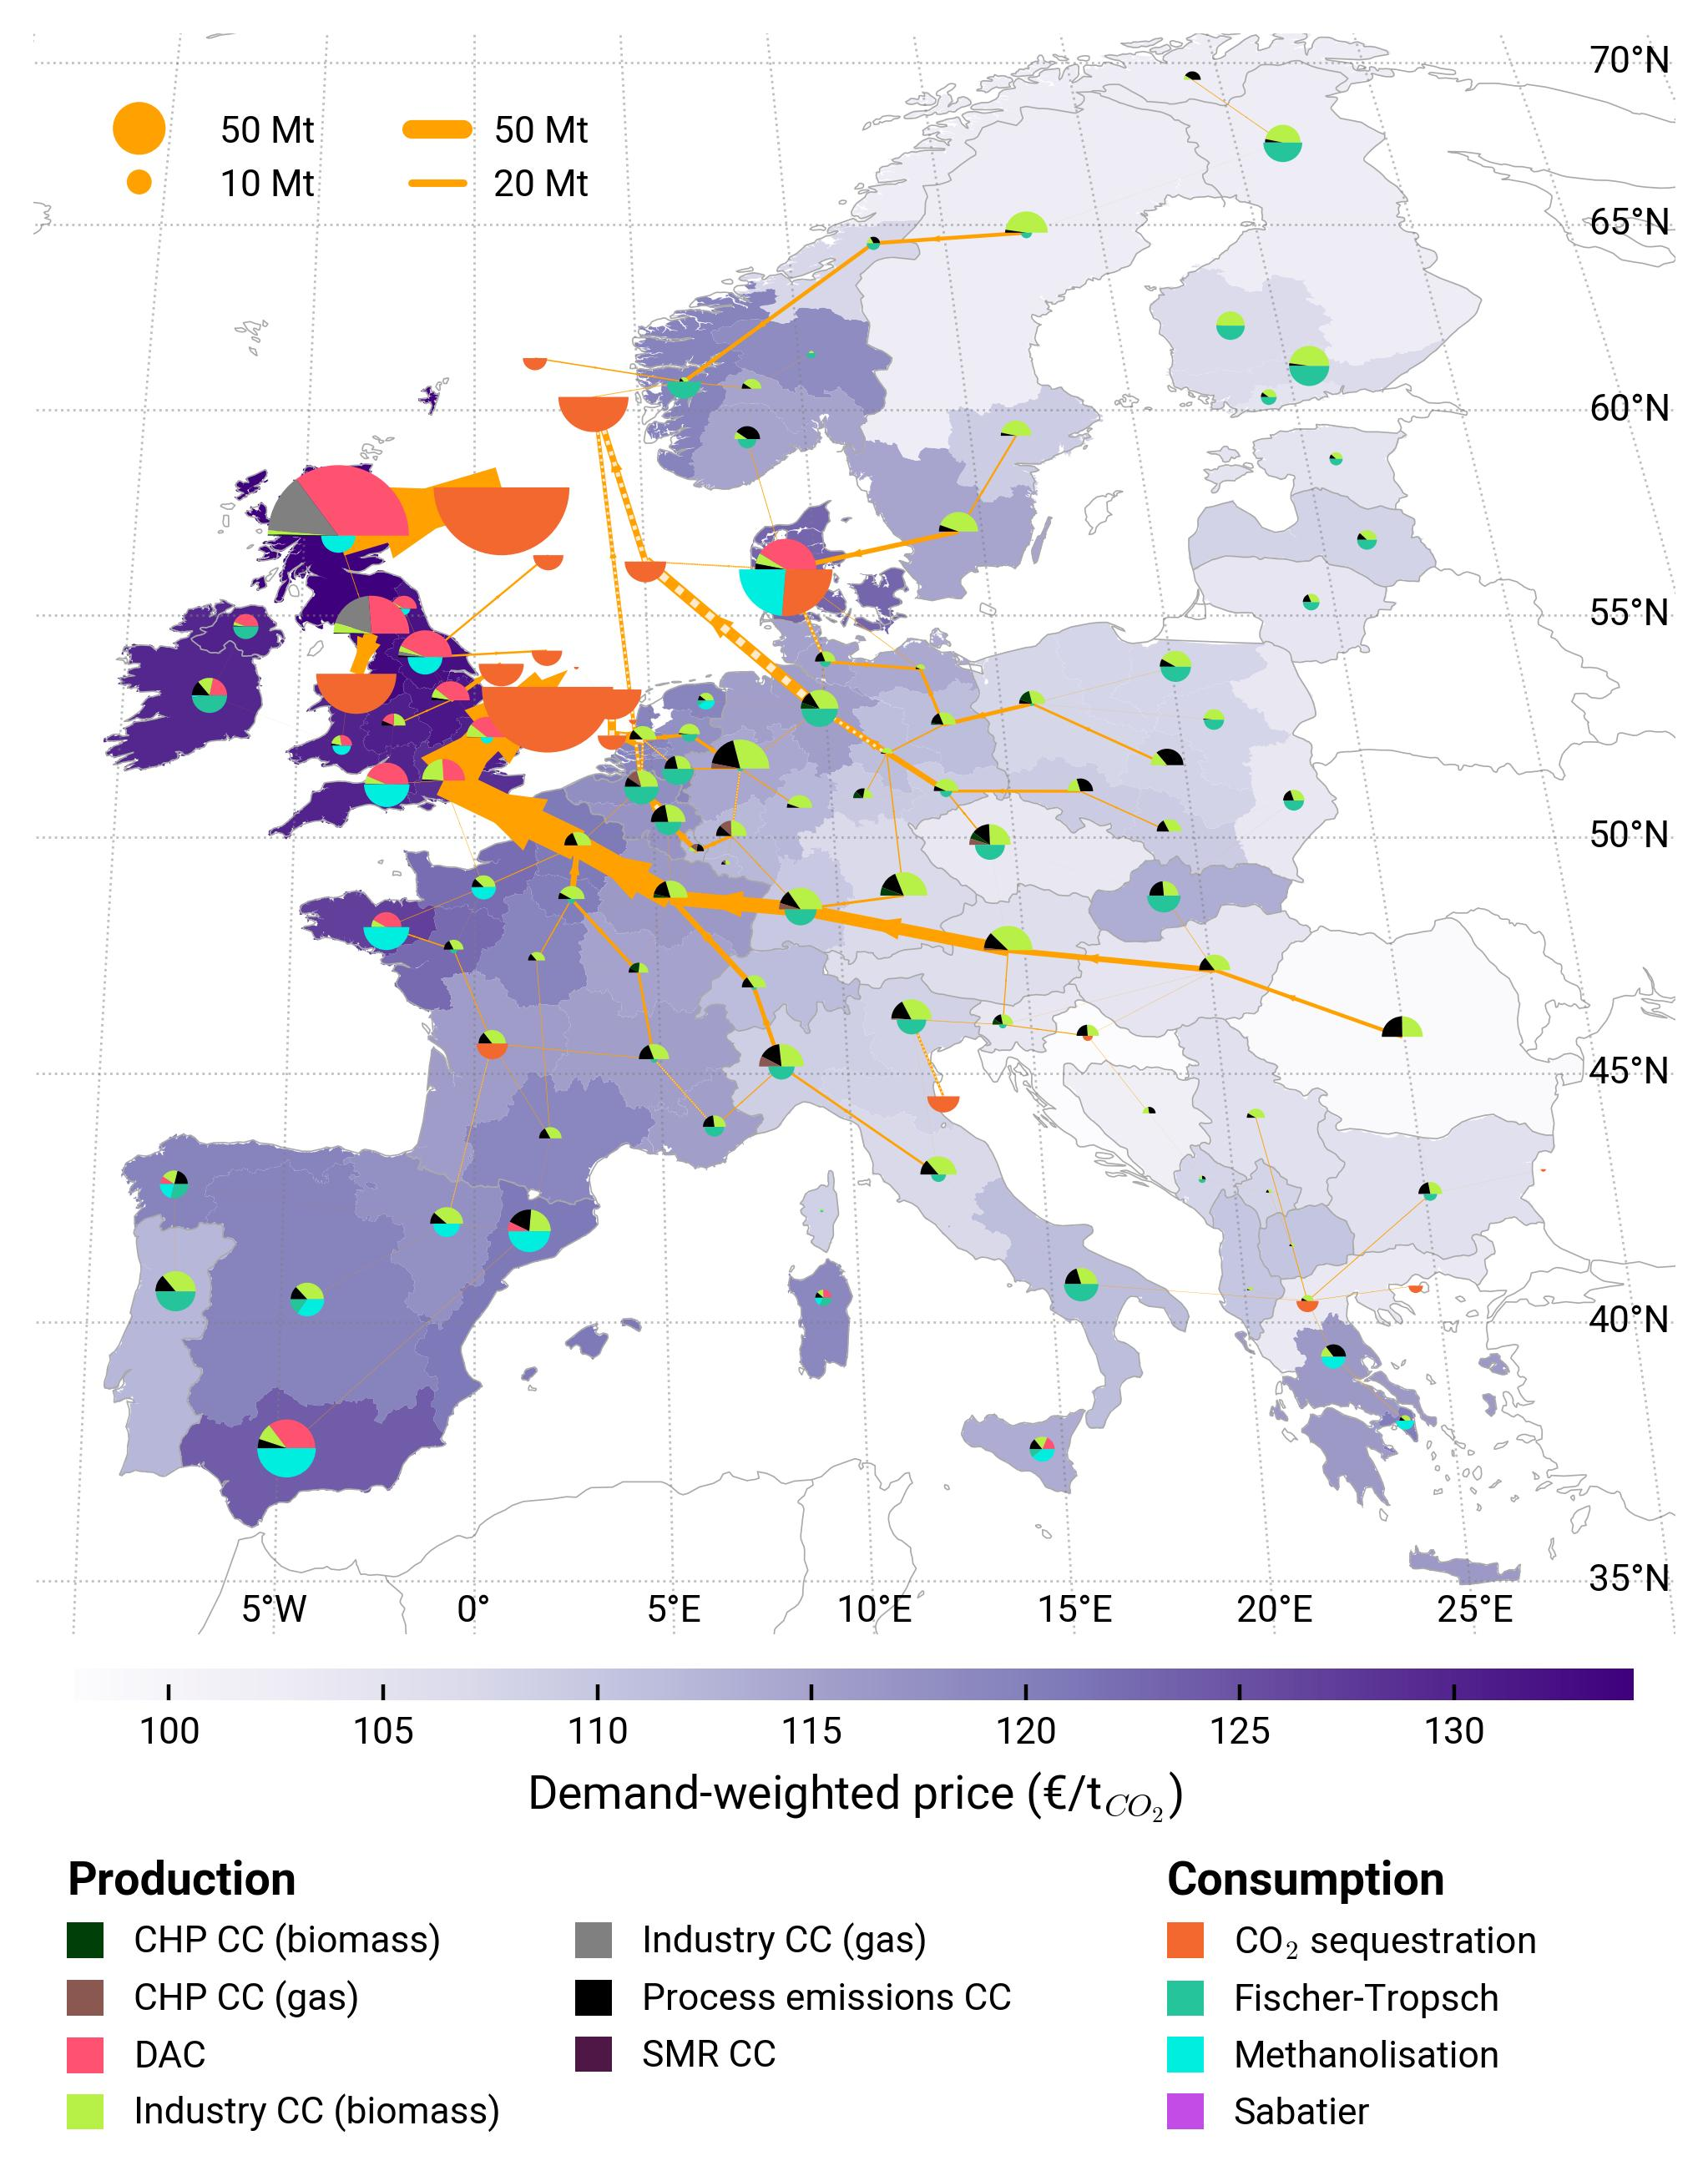
\includegraphics[width=1\textwidth]{maps/pcipmi-national-international-expansion/base_s_adm___2050-balance_map_co2_stored} 
      \vspace{-0.7cm}
      \caption{\ce{CO2} regional balances and flows.}
      \label{fig:PCI-in_lt_2050_co2}
  \end{subfigure}
  \caption{\textit{PCI-in} long-term scenario (2050) --- Regional distribution of \ce{H2} and \ce{CO2} production, utilisation, storage, and transport.}
  \label{fig:PCI-in_lt_2050}
\end{figure*}

\clearpage

\subsubsection{Central Planning}
\begin{figure*}[htbp]
  \centering
  \begin{subfigure}[t]{0.49\textwidth}
      \vspace{0pt}
      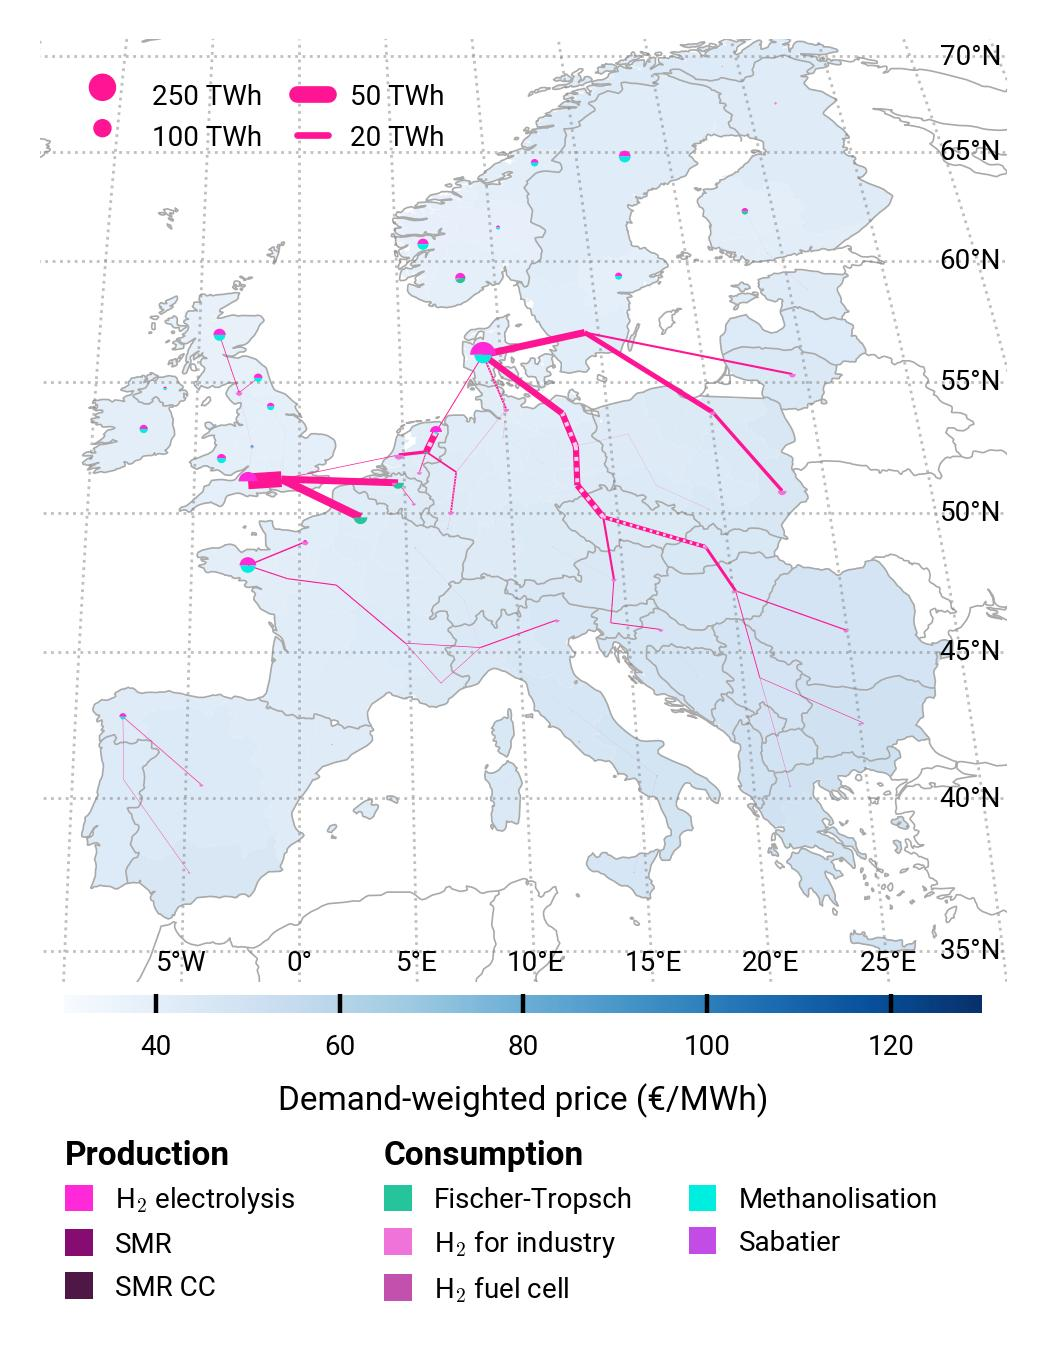
\includegraphics[width=1\textwidth]{maps/greenfield-pipelines/base_s_adm___2030-balance_map_H2}
      \vspace{-0.5cm}
      \caption{\ce{H2} regional balances and flows.}
      \label{fig:CP_lt_2030_h2}
  \end{subfigure}
  \hfill
  \begin{subfigure}[t]{0.49\textwidth}
      \vspace{0pt}
      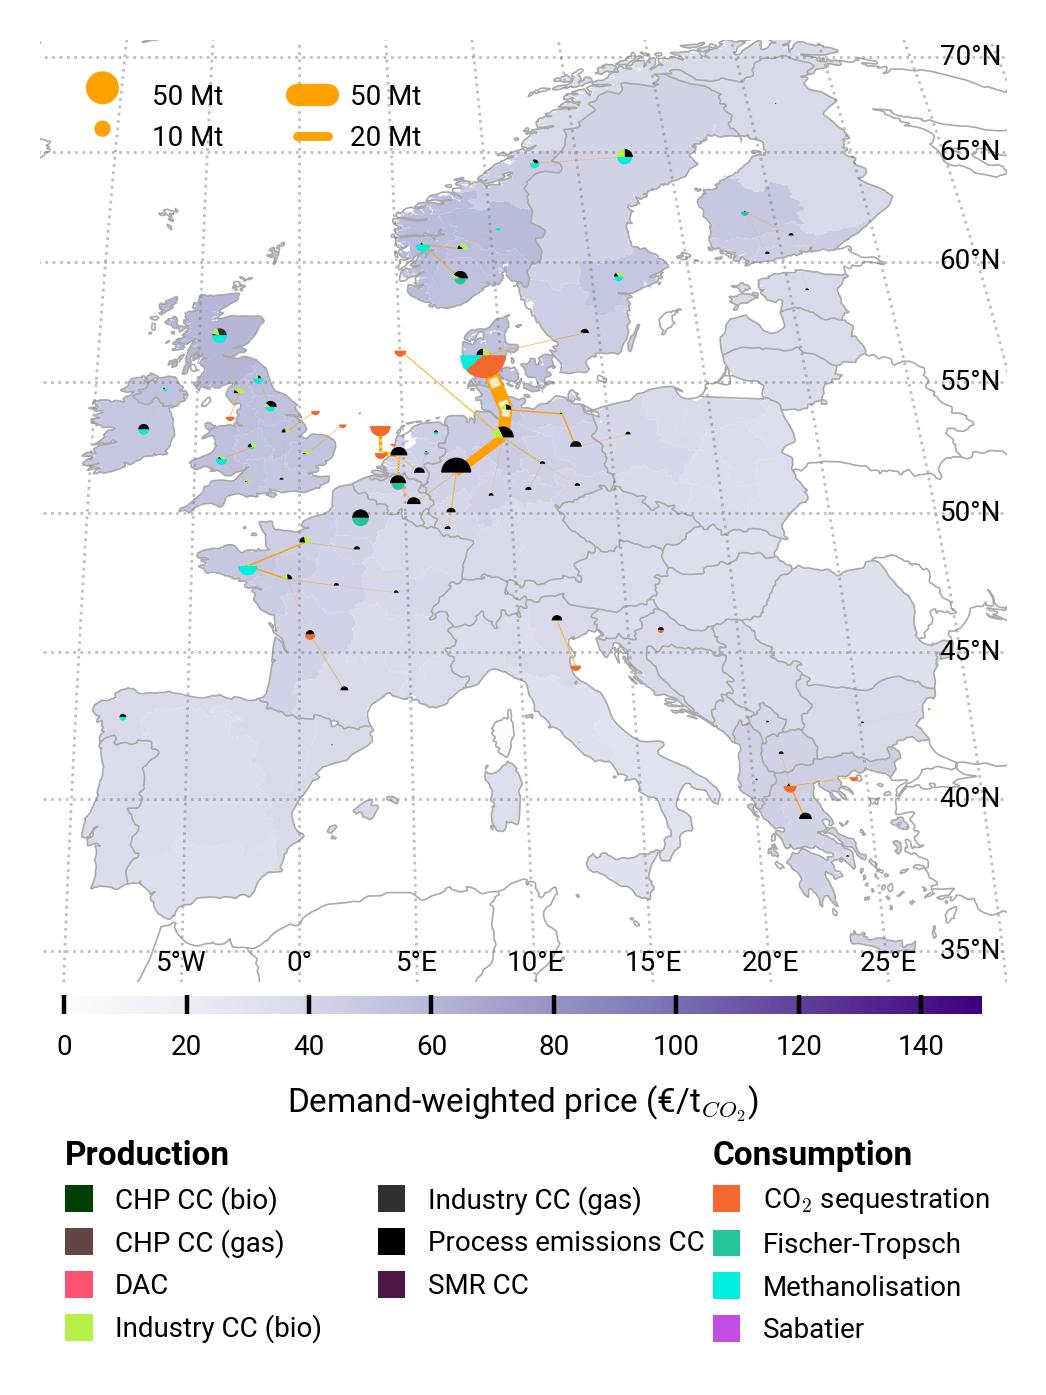
\includegraphics[width=1\textwidth]{maps/greenfield-pipelines/base_s_adm___2030-balance_map_co2_stored} 
      \vspace{-0.7cm}
      \caption{\ce{CO2} regional balances and flows.}
      \label{fig:CP_lt_2030_co2}
  \end{subfigure}
  \caption{\textit{Central Planning} long-term scenario (2030) --- Regional distribution of \ce{H2} and \ce{CO2} production, utilisation, storage, and transport.}
  \label{fig:CP_lt_2030}
\end{figure*}

\begin{figure*}[htbp]
  \centering
  \begin{subfigure}[t]{0.49\textwidth}
      \vspace{0pt}
      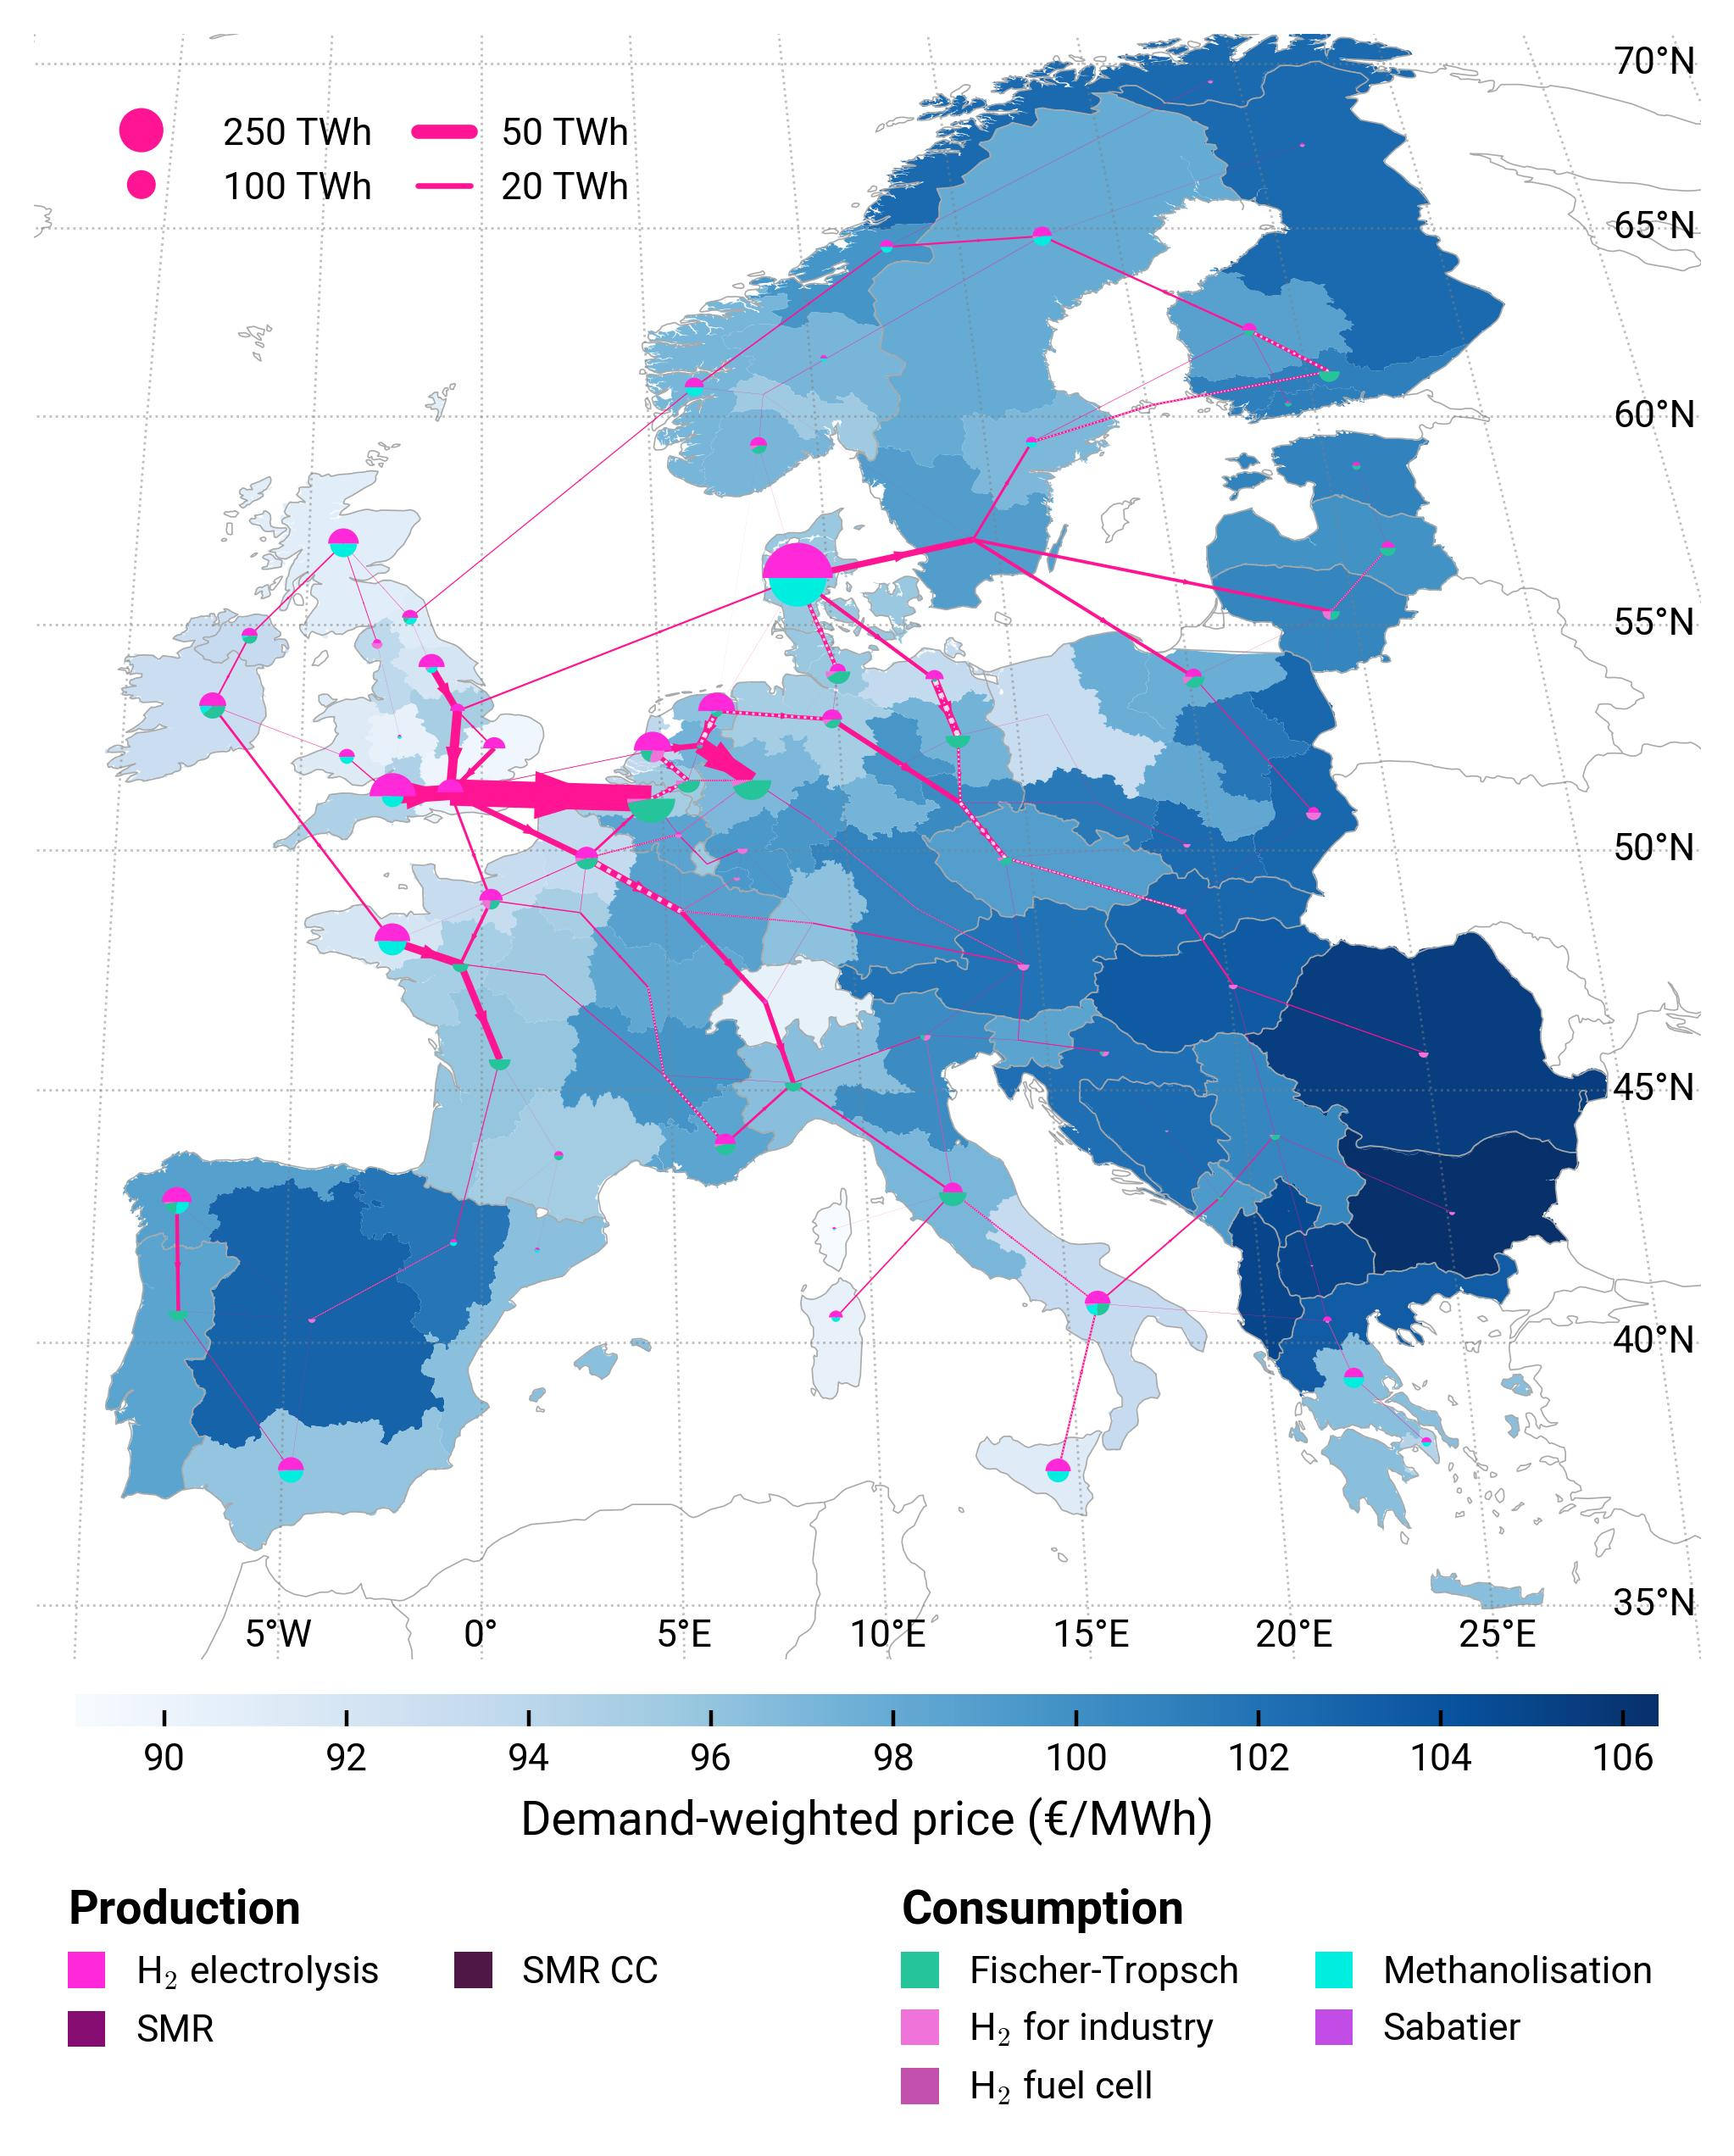
\includegraphics[width=1\textwidth]{maps/greenfield-pipelines/base_s_adm___2040-balance_map_H2}
      \vspace{-0.5cm}
      \caption{\ce{H2} regional balances and flows.}
      \label{fig:CP_lt_2040_h2}
  \end{subfigure}
  \hfill
  \begin{subfigure}[t]{0.49\textwidth}
      \vspace{0pt}
      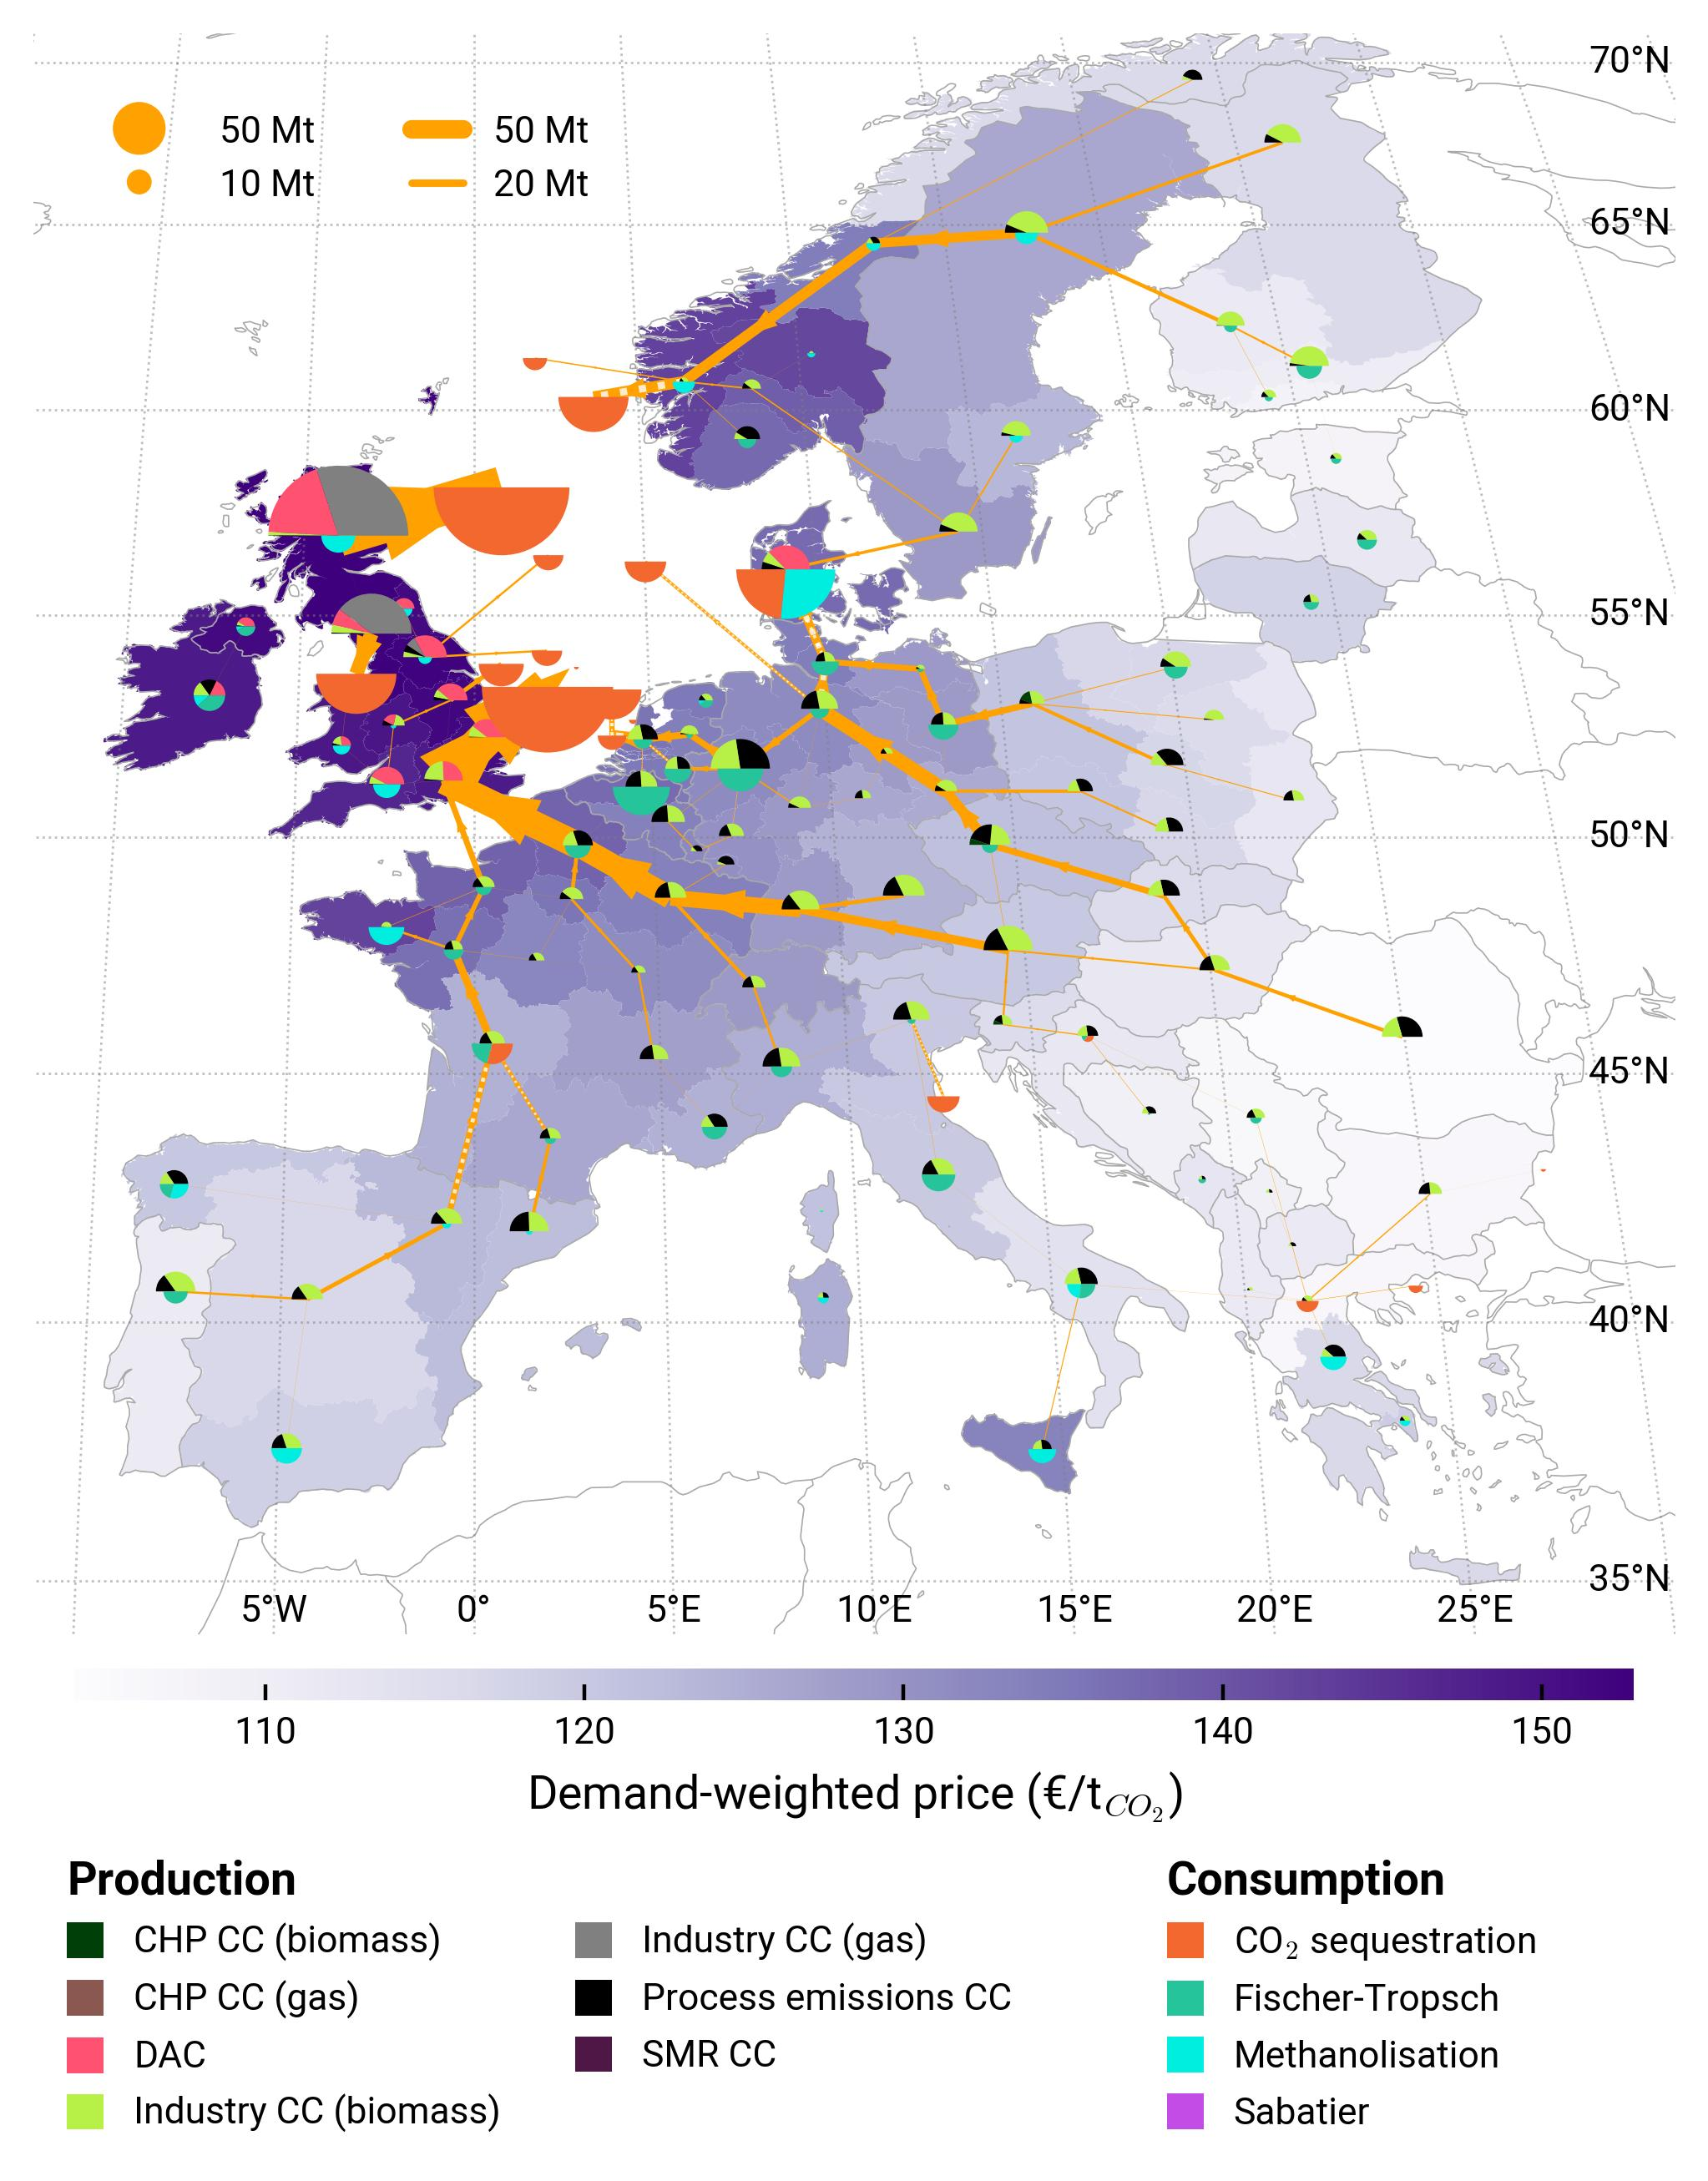
\includegraphics[width=1\textwidth]{maps/greenfield-pipelines/base_s_adm___2040-balance_map_co2_stored} 
      \vspace{-0.7cm}
      \caption{\ce{CO2} regional balances and flows.}
      \label{fig:CP_lt_2040_co2}
  \end{subfigure}
  \caption{\textit{Central Planning} long-term scenario (2040) --- Regional distribution of \ce{H2} and \ce{CO2} production, utilisation, storage, and transport.}
  \label{fig:CP_lt_2040}
\end{figure*}

\begin{figure*}[htbp]
  \centering
  \begin{subfigure}[t]{0.49\textwidth}
      \vspace{0pt}
      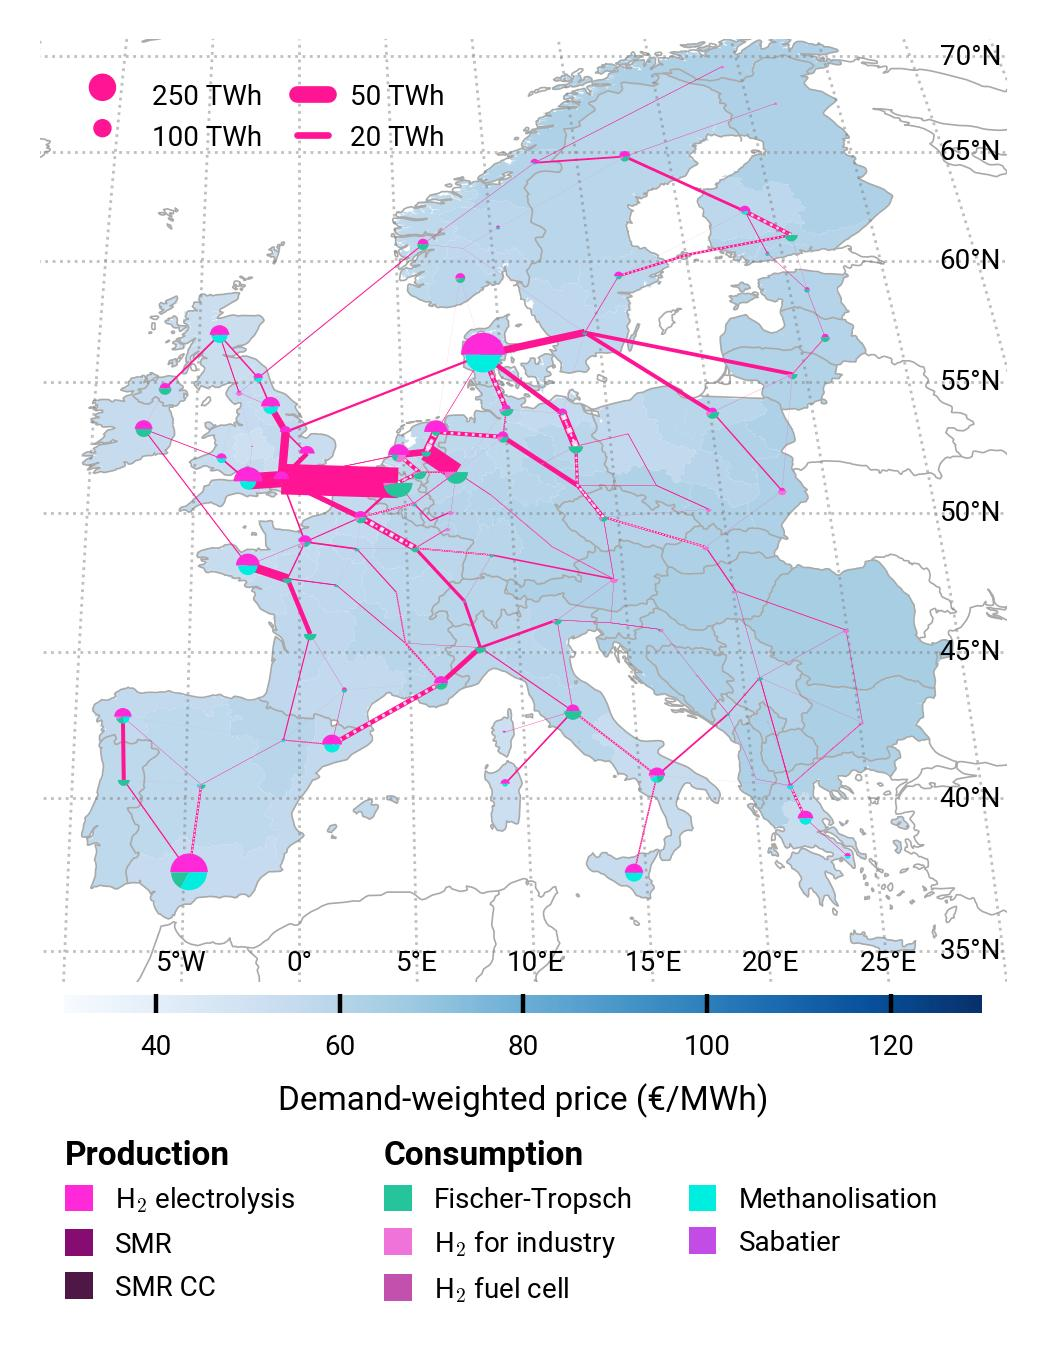
\includegraphics[width=1\textwidth]{maps/greenfield-pipelines/base_s_adm___2050-balance_map_H2}
      \vspace{-0.5cm}
      \caption{\ce{H2} regional balances and flows.}
      \label{fig:CP_lt_2050_h2}
  \end{subfigure}
  \hfill
  \begin{subfigure}[t]{0.49\textwidth}
      \vspace{0pt}
      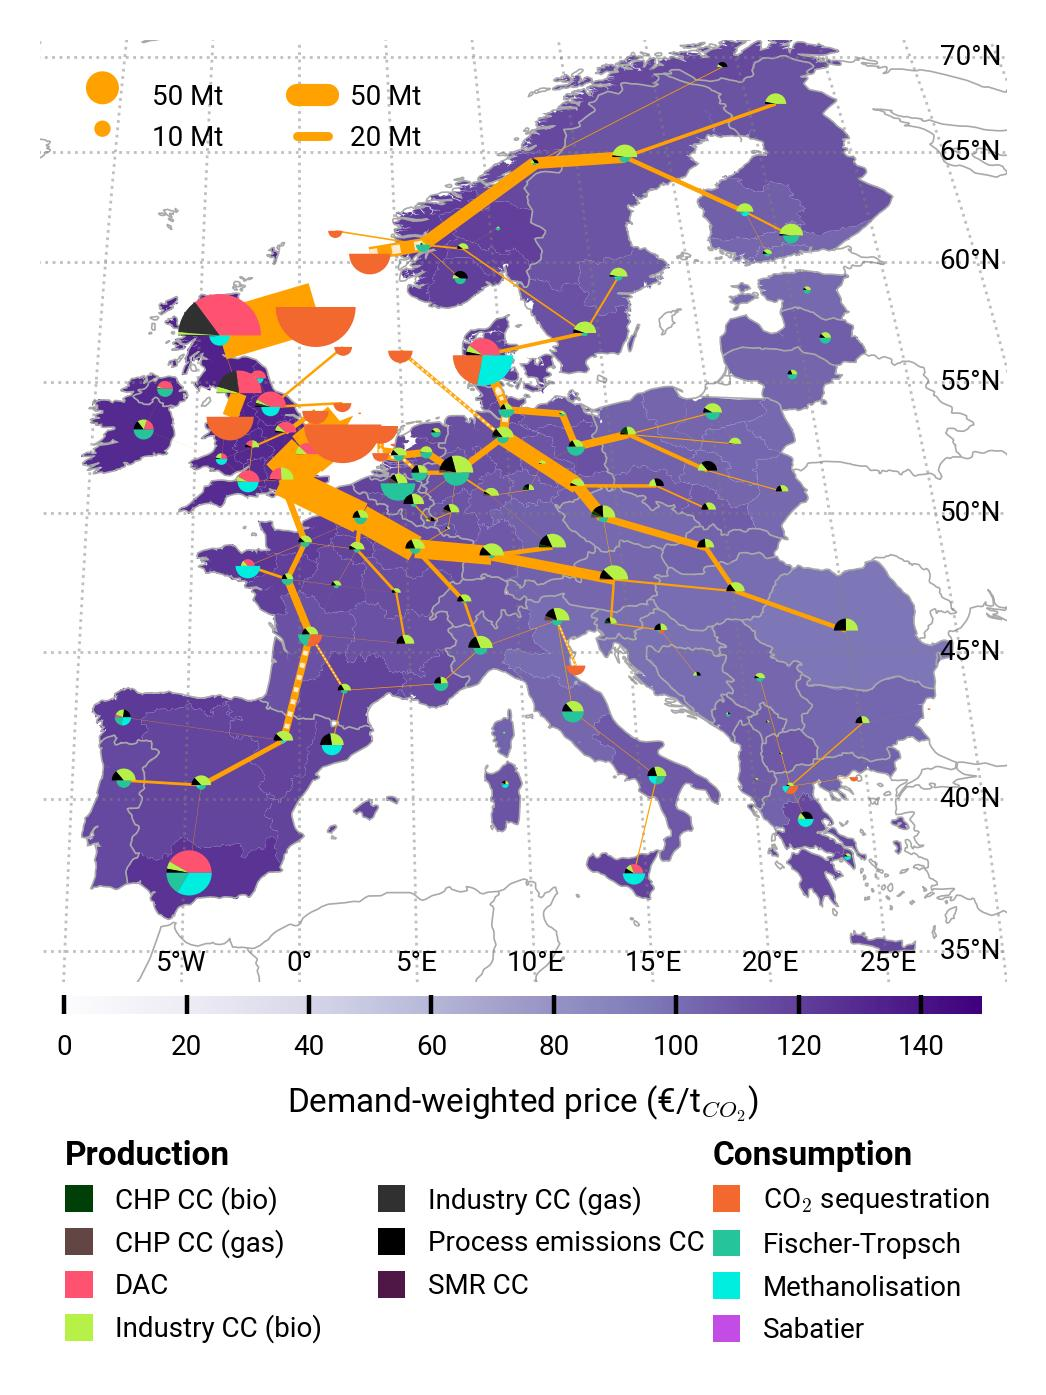
\includegraphics[width=1\textwidth]{maps/greenfield-pipelines/base_s_adm___2050-balance_map_co2_stored} 
      \vspace{-0.7cm}
      \caption{\ce{CO2} regional balances and flows.}
      \label{fig:CP_lt_2050_co2}
  \end{subfigure}
  \caption{\textit{Central Planning} long-term scenario (2050) --- Regional distribution of \ce{H2} and \ce{CO2} production, utilisation, storage, and transport.}
  \label{fig:CP_lt_2050}
\end{figure*}

\clearpage
\bibliographystyle{elsarticle-num} 
\bibliography{references.bib}

\end{document}

\endinput
%%
%% End of file `elsarticle-template-num.tex'.


%% Template related

% \section{Example Section}
% \label{sec1}
% %% Labels are used to cross-reference an item using \ref command.

% Section text. See Subsection \ref{subsec1}.

% %% Use \subsection commands to start a subsection.
% \subsection{Example Subsection}
% \label{subsec1}

% Subsection text.

% %% Use \subsubsection, \paragraph, \subparagraph commands to 
% %% start 3rd, 4th and 5th level sections.
% %% Refer following link for more details.
% %% https://en.wikibooks.org/wiki/LaTeX/Document_Structure#Sectioning_commands

% \subsubsection{Mathematics}
% %% Inline mathematics is tagged between $ symbols.
% This is an example for the symbol $\alpha$ tagged as inline mathematics.

% %% Displayed equations can be tagged using various environments. 
% %% Single line equations can be tagged using the equation environment.
% \begin{equation}
% f(x) = (x+a)(x+b)
% \end{equation}

% %% Unnumbered equations are tagged using starred versions of the environment.
% %% amsmath package needs to be loaded for the starred version of equation environment.
% \begin{equation*}
% f(x) = (x+a)(x+b)
% \end{equation*}

% %% align or eqnarray environments can be used for multi line equations.
% %% & is used to mark alignment points in equations.
% %% \\ is used to end a row in a multiline equation.
% \begin{align}
%  f(x) &= (x+a)(x+b) \\
%       &= x^2 + (a+b)x + ab
% \end{align}

% \begin{eqnarray}
%  f(x) &=& (x+a)(x+b) \nonumber\\ %% If equation numbering is not needed for a row use \nonumber.
%       &=& x^2 + (a+b)x + ab
% \end{eqnarray}

% %% Unnumbered versions of align and eqnarray
% \begin{align*}
%  f(x) &= (x+a)(x+b) \\
%       &= x^2 + (a+b)x + ab
% \end{align*}

% \begin{eqnarray*}
%  f(x)&=& (x+a)(x+b) \\
%      &=& x^2 + (a+b)x + ab
% \end{eqnarray*}

% %% Refer following link for more details.
% %% https://en.wikibooks.org/wiki/LaTeX/Mathematics
% %% https://en.wikibooks.org/wiki/LaTeX/Advanced_Mathematics

% %% Use a table environment to create tables.
% %% Refer following link for more details.
% %% https://en.wikibooks.org/wiki/LaTeX/Tables
% \begin{table}[t]%% placement specifier
% %% Use tabular environment to tag the tabular data.
% %% https://en.wikibooks.org/wiki/LaTeX/Tables#The_tabular_environment
% \centering%% For centre alignment of tabular.
% \begin{tabular}{l c r}%% Table column specifiers
% %% Tabular cells are separated by &
%   1 & 2 & 3 \\ %% A tabular row ends with \\
%   4 & 5 & 6 \\
%   7 & 8 & 9 \\
% \end{tabular}
% %% Use \caption command for table caption and label.
% \caption{Table Caption}\label{fig1}
% \end{table}


% %% Use figure environment to create figures
% %% Refer following link for more details.
% %% https://en.wikibooks.org/wiki/LaTeX/Floats,_Figures_and_Captions
% \begin{figure}[t]%% placement specifier
% %% Use \includegraphics command to insert graphic files. Place graphics files in 
% %% working directory.
% \centering%% For centre alignment of image.
% \includegraphics{example-image-a}
% %% Use \caption command for figure caption and label.
% \caption{Figure Caption}\label{fig1}
% %% https://en.wikibooks.org/wiki/LaTeX/Importing_Graphics#Importing_external_graphics
% \end{figure}

%% For citations use: 
%%       \cite{<label>} ==> [1]

%%
% Example citation, See \cite{lamport94}.

%% If you have bib database file and want bibtex to generate the
%% bibitems, please use

%% else use the following coding to input the bibitems directly in the
%% TeX file.

%% Refer following link for more details about bibliography and citations.
%% https://en.wikibooks.org/wiki/LaTeX/Bibliography_Management

% \begin{thebibliography}{00}

% %% For numbered reference style
% %% \bibitem{label}
% %% Text of bibliographic item

% \bibitem{lamport94}
%   Leslie Lamport,
%   \textit{\LaTeX: a document preparation system},
%   Addison Wesley, Massachusetts,
%   2nd edition,
%   1994.

% \end{thebibliography}